\documentclass[12pt]{article}

% TEMPLATE DEFAULT PACKAGES
\usepackage{amssymb,amsmath,amsfonts,eurosym,geometry,ulem,graphicx,color,setspace,sectsty,comment,natbib,pdflscape,array,adjustbox}

% ADDED PACKAGES FOR THIS MANUSCRIPT
\usepackage{palatino,newtxmath,multirow,titlesec,threeparttable,tabu,booktabs,titlesec,threeparttable,mathtools,bm,bbm,subcaption,pdflscape,tcolorbox,mathrsfs,tikz,float,longtable}
% endfloat,
% \usepackage[capposition=top]{floatrow}
\usepackage{tikzpagenodes}
\usepackage{pbox}

\usepackage{afterpage}
\usepackage[hyphens]{url}
\usepackage[margin=1cm]{caption}

\usepackage[draft]{hyperref}
\newcommand{\tim}{$\,\times\,$}
% FIGURES & TABLES CAPTION STYLING
\captionsetup[figure]{labelfont={bf},name={Figure},labelsep=period}
\captionsetup[table]{labelfont={bf},name={Table},labelsep=period}

% SECTION TITLE SETTINGS
\titlelabel{\thetitle.\enskip}
\titleformat*{\section}{\large\bfseries}
\titleformat*{\subsection}{\normalsize\bfseries}

% COLUMN TYPES
\newcolumntype{L}[1]{>{\raggedright\let\newline\\\arraybackslash\hspace{0pt}}m{#1}}
\newcolumntype{C}{>{\centering\arraybackslash}p{5.2em}}
\newcolumntype{D}{>{\centering\arraybackslash}p{5em}}
\newcolumntype{E}{>{\centering\arraybackslash}p{6em}}
\newcolumntype{G}{>{\centering\arraybackslash}p{8em}}
\newcolumntype{Z}{>{\centering\arraybackslash}p{10em}}
\newcolumntype{R}[1]{>{\raggedleft\let\newline\\\arraybackslash\hspace{0pt}}m{#1}}


% MARGINS AND SPACING
\normalem
\geometry{left=1.1in,right=1.1in,top=1.0in,bottom=1.0in}
\setlength{\parskip}{2.5pt}


% SPECIAL CELL 
\newcommand{\specialcell}[2][c]{%
	\begin{tabular}[#1]{@{}l@{}}#2\end{tabular}}

% NO INDENT ON FOOTNOTES
\usepackage[hang,flushmargin]{footmisc}


\newcommand{\regtextfirst}{
Mean pre and post are average outcomes across all areas pre and post project construction.  Standard errors (in parentheses) are clustered at the project level.  P-values [in brackets] adjust for multiple hypothesis testing using the Bonferroni method and inform the superscripts, \textsuperscript{c} p$<$0.10,\textsuperscript{b} p$<$0.05,\textsuperscript{a} p$<$0.01 \,\,
}

\newcommand{\regtext}{
Mean pre and post are average outcomes  across all areas pre and post project construction.   Although not displayed in the table, specifications also include separate effects for 0.5 km rings from 0 to 4 km and results are available upon request.  Standard errors (in parentheses) are clustered at the project level.  P-values [in brackets] adjust for multiple hypothesis testing using the Bonferroni method and inform the coefficient superscripts, \textsuperscript{c} p$<$0.10,\textsuperscript{b} p$<$0.05,\textsuperscript{a} p$<$0.01 \,\,
}

\newcommand{\ballparktext}{
	``Footprint'' sums the footprint effect across plots within constructed projects.
	``Spillover'' sums the neighborhood effect (0-.5 km) across plots nearby constructed projects.
	``Total'' sums ``Footprint'' and ``Spillover'' effects.
}

%%% EDIT COMMANDS %%%
\newcommand{\rv}{}
\newcommand{\rt}{\textbf{Heavily Revised Table: }}
\newcommand{\nt}{\textbf{New Table: }}
\newcommand{\ns}{\textbf Heavily Revised Section: }



\begin{document}

\begin{titlepage} 
\title{{Public Housing Spillovers:  Evidence from South Africa}\thanks{We are grateful to Andrew Foster, Daniel Bjorkegren, Matthew Turner, Jesse Shapiro, Brian Knight, and John Friedman for their feedback and advice.  We also thank Adelaide Steedley and the Centre for Affordable Housing and Finance in Africa as well as GeoTerraImage for generous research guidance and for providing data without which this project would not have been possible.  Any opinions and conclusions expressed herein are those of the authors and do not necessarily represent the views of the Federal Trade Commission or its Commissioners.}}
\author{\\[3em] Benjamin H. Bradlow\thanks{Department of Sociology, Princeton University, Princeton, NJ. E-mail: bhbradlow@princeton.edu}\\
 Stefano Polloni\thanks{Palmetto, Charleston, SC.   E-mail: stefano.polloni@palmetto.com}\\ 
  William Violette\thanks{Federal Trade Commission, Washington, DC. E-mail: william.j.violette@gmail.com} \\
 \\ 
  }
% \vspace{30mm}
\date{\vspace{5mm}This Version: \today}
\maketitle
\begin{abstract}

%%% STATEMENT HERE!  

	%Does subsidized housing improve neighborhood quality in developing countries? 

	% Public housing projects may complement local housing investments as well as substitute for existing housing, especially low-quality slums.  

	% We estimate the direct and spillover effects of large public housing projects in South Africa using aerial measures of housing density, property transaction records, and census data.  

% affects population density, construction of private housing, and access to basic services

	% We estimate the effects of building public housing projects on urban development both inside project footprints as well as in surrounding areas in South Africa.  To identify effects, we compare changes in outcomes for 166 projects that are successfully constructed to 140 projects that remain planned but not constructed.  


Can place-based policies promote urban development beyond their footprints?  We estimate the spillover effects of public housing projects in South Africa by comparing changes near 166 projects that were successfully constructed to changes near 140 projects that were planned but not constructed.  \rv{Constructed projects triple the amount of formal housing inside their footprints and lead to one new informal house being built for every three new formal houses. These effects extend beyond project footprints, with increases in both formal and informal housing detected up to 500m from the targeted areas.  The findings are consistent with projects generating positive housing externalities}.


 % as well as both formal and informal housing nearby.
	% Projects are large and successful, delivering over 1,000 houses per project.  
	%  projects before and after scheduled construction, we find that projects generate growth with their footprints exceeding 
	% measure changes in housing density, property transaction records, and census data
	% , , both within 
	% 1,000 houses and 3,000 people per project.  Nearby projects, we estimate positive spillover effects that further contribute nearly 170 houses and 500 people per project.  

	% \footnote{We may want to establish the general question, object of study. Something like: “While public housing projects are generally assumed to improve welfare by virtue of providing improved housing conditions, we find wide variation in how such programs impact contemporary slum development in rapidly urbanizing contexts.}

%%%%%% MACRO THE HETEROGENEITY DISTANCE
%Within project footprints, housing quality improves and subsidized formal structures successfully crowd-out slums. 


\vspace{.1in}
\textbf{Keywords:} housing policy; place-based policy; urban development.\\
% \vspace{0in}\\
\textbf{JEL Codes:} O18; O22; H4; R3.  \\
\bigskip
\end{abstract}
\setcounter{page}{0}
\thispagestyle{empty}
\end{titlepage}
% \pagebreak \newpage

\spacing{1.4}
\section{Introduction} \label{sec:introduction}



30\% of urban populations in developing countries live in slums characterized by overcrowding and informal houses made of non-durable material \citep{mdg}.  Dense slums often produce congestion and unsanitary conditions, which discourage new housing construction and infrastructure investments \citep{marx2013slums}.  To break this cycle, cities target slums with place-based policies such as land titling, slum upgrading, and public housing projects.  Across Africa, governments have provided over 5.4 million houses from 2,500 in Benin to 3 million in South Africa \citep{bah2018housing}.  

In developing cities, slum conditions may amplify the welfare effects of place-based policies.  Policies that upgrade slums with improved housing may yield additional benefits by reducing congestion, improving sanitation, and inviting infrastructure investment.  Policies can also have unintended consequences by attracting new slum growth.  For example, low-density public housing projects may leave room for households to build low-quality houses in the backyards of project houses \citep{Brueckner2018backyarding}.  Dense backyard housing may recreate unsanitary conditions and depress neighborhood property investment.  The net effects of these policies remain an empirical question that has implications for designing place-based policies in developing cities.

This paper asks how public housing projects affect population growth, housing development, and public services in areas within project footprints as well as areas nearby project footprints.  \rv{We examine these effects in the context of South African housing projects.  While South Africa has a higher average income than many of its sub-Saharan counterparts, housing projects are often located in undeveloped areas that share many similarities with urban slums across Africa.\footnote{\rv{Compared to its low-income, sub-Saharan neighbors, South Africa is unique in its ability to fund large-scale housing programs \citep{bah2018housing}.}}  Annually since 1994, the South African government acquires parcels of land and contracts the construction of many housing projects.  Projects consist of (1) building neighborhoods of new single-story, two-room houses each on their own plot of land, (2) allocating full ownership of houses to recipient households, and (3) servicing houses with basic infrastructure including water, electricity, community centers, and other complementary investments.  Housing projects range widely in size from a few dozen to several hundred houses per project.}

\rv{We compile detailed spatial data in 2001 and 2011 for the Johannesburg metro-area including household census data, deeds records of formal housing transactions, and a remote-sensed survey of all buildings.\footnote{\rv{Our data do not cover Pretoria.}}  These data allow us to measure the medium-term outcomes for housing projects built between 2001 and 2011.   The building survey provides a novel measure of slum growth by distinguishing between formal and informal house types.  Our main outcomes are population, formal and informal housing density, formal house prices, infrastructure investments, and demographics.} To measure impacts across multiple spatial datasets, we create a uniform unit of analysis by overlaying gridded 100 by 100m plots of land across all areas within 4 km of projects and computing average measures within each plot.\footnote{For spatial measures that partially overlap with plots (such as census enumerator areas), we attribute measures to plots based on their greatest area of overlap.} 

Our empirical strategy compares changes in outcomes for exposure to 166 constructed projects to changes in outcomes for exposure to 140 planned, but unconstructed projects.  \rv{We measure project exposure for each plot of land based on the area that each plot overlaps with project footprints.  For plots outside of project footprints, we calculate the area for which each plot's immediate neighborhood overlaps with project footprints.  Since housing projects are often clustered near each other, the measure allows plots to be exposed to multiple projects at varying intensities.}  

\rv{The empirical strategy addresses two main challenges in measuring the impacts of housing projects.  First, projects are often located not only in poor neighborhoods, but also on relatively undeveloped plots of land within these neighborhoods.  Comparing projects to neighboring areas would likely capture these preexisting differences.  Our strategy controls for these differences because constructed and unconstructed projects are often located on similar types of land plots in similar types of neighborhoods.  Second, projects are often located in rapidly growing cities with high demand for housing.  Measuring the evolution of project areas would likely also capture urban growth that is unrelated to the projects.  Our strategy controls for trends in urban development by comparing relative growth across areas with constructed projects and areas with unconstructed projects.}

The empirical strategy identifies the causal effect of housing projects under the assumption that plots exposed to constructed projects would have evolved in the same way as plots similarly exposed to unconstructed projects in the absence of construction.  Our approach leverages how planned housing projects must satisfy many procedural hurdles to be eligible for construction (ie. environmental impact assessments, zoning approvals, infrastructure plans), which \rv{may be relatively uncorrelated} with local trends in development.  

\rv{We observe that in the pre-period, areas near constructed projects have more houses and people than areas near unconstructed projects.  This pattern is consistent with mismeasurement of construction status where some projects were actually completed prior to our pre-period data.  This mismeasurement would lead comparisons of constructed and unconstructed projects to underestimate the effect of project construction.}  Another explanation is that local authorities prioritize dense, slum areas for project construction.  To address these concerns, we show that our main results are similar to analyzing only project footprints without houses in the pre-period or balancing on pre-period characteristics.  We also find limited evidence of pre-trends in census outcomes.


\rv{We find that constructed projects largely succeed in their three goals of building, allocating, and servicing project houses.  The numbers of formal houses and people living in formal houses triple in constructed projects relative to unconstructed projects.  New formal houses are well-serviced with basic utilities and largely resemble other formal houses in project areas.  Projects do not seem to change the demographics of people living in formal housing in project areas.  } We also estimate that constructed projects invite growth of informal backyard houses, which may partially undermine South Africa's goals to ``ensure the elimination and prevention of slums and slum conditions.''\footnote{See \cite{housingact}.}  Together, these effects translate into growth of over \rv{660 new formal houses and 3,060 people per project} within their footprints.

\rv{We also observe that projects have the unintended consequence of stimulating large increases in informal housing within project footprints. One new informal house is built for every three new formal houses.  The growth of informal housing is driven entirely by informal dwellings built in the backyards of formal dwellings\citep{Brueckner2018backyarding}.\footnote{Qualitative interviews with national and local government housing officials that we conducted between 2015 and 2017 suggest that housing subsidy programs are viewed as being in contradiction to an outcome of densifying backyard shacks.} }

\rv{We then estimate spillover effects nearby projects.}  Between 0 and 0.5 km from project footprints, we find positive effects that are statistically significant for population and house growth with informal houses outpacing formal houses.   \rv{Estimates imply that on average, each project invites nearby growth of 66 formal houses, 103 informal, backyard houses, and 27 informal, non-backyard houses.}  These results are consistent with housing projects supporting government goals ``to use money available for housing development in a manner which stimulates private investment in, and the contributions of individuals to housing development.''\footnote{See \cite{housingact}.} 

\rv{We estimate that prices for formal housing transactions increase by 9\% up to 0.5 km from project footprints although this result is statistically indistinguishable from zero.  This effect is similar to previous price estimates in the literature, which range from 6.5\% to 15\% in low-income US neighborhoods to 12\% in middle-income neighborhoods in Uruguay.\footnote{See \cite{diamond2019wants} and \cite{baum2009effects} for US Low Income Housing Tax Credit estimates.  See \cite{gonzalez2022spillover} for public housing estimates from Uruguay.}  Our effect differs from the 2.5\% decrease in prices observed in high income US neighborhoods.\footnote{See \citep{diamond2019wants}.}  Given that South African housing projects are located in relatively low-income neighborhoods, our price effects are largely consistent with the literature. }

\rv{To explain positive spillover effects, we consider three potential mechanisms.}
\begin{enumerate}
  \item \rv{Project infrastructure investments including electricity and water may also benefit nearby houses.  However, we observe little change in access to basic services among nearby houses.}
  \item \rv{Buildings identified as businesses increase within projects, which may invite employees to locate nearby projects.  However, we detect no changes in income, employment, or business growth nearby projects.}
  \item \rv{Projects may produce positive housing externalities for surrounding households (\cite{rossi2010housing}; \cite{diamond2019wants}).  For example, neighbors may benefit from social interactions, improved perceptions of safety, and community development.  Observed increases in both formal and informal houses as well as formal prices are consistent with positive housing externalities.}
\end{enumerate}
\rv{On the whole, we find that infrastructure investment and business growth within projects may not extend to neighboring areas.  Positive housing externalities remain a plausible explanation for the positive housing spillovers observed in our analysis.}

This paper contributes to growing research on place-based policies.  Studies in the US compare changes in outcomes either (1) near versus far from project areas\footnote{See \cite{rossi2010housing,hornbeck2017creative}, and \cite{diamond2019wants}.} or (2) in constructed versus planned, but unconstructed project areas.\footnote{See \cite{busso2013assessing} and \cite{kline2013local}.}  Most closely related to our work, \cite{diamond2019wants} find that public housing projects in the US increase housing prices in low-income neighborhoods and decrease housing prices in high-income neighborhoods.  \rv{Since we focus on a developing context with pervasive informal housing, our study differs in two main ways.  First, in these settings, it may be important to account for spatial outcomes within project footprints such as backyard housing.  Second, to the extent that informal housing grows in response to place-based policies and is itself a negative amenity, informal housing may undermine policy goals of producing positive amenities.}

In developing countries, researchers often lack panel data and instead, rely on cross-sectional comparisons to study spillover effects of housing and urban development policies.  In Tanzania, \cite{baruah2017planning} observe that areas near sites-and-services programs have better housing quality than similar, untreated areas.  Using a similar design \rv{to study slum-upgrading} in Jakarta, Indonesia, \cite{harari2018slum} find declines in local land values and levels of formalization.  \cite{gechter2020spatial} link changes in Mumbai's zoning laws to formal housing development and higher nearby property prices.   \rv{Our study contributes to this literature by studying public housing projects using spatial panel data.}

Our study also relates to recent research on South Africa's national housing program focusing on outcomes for direct beneficiaries of project houses.  Using household surveys, studies estimate the effect of receiving a project house on women's labor supply: \cite{picarelli2019there}  finds negative effects nationally while \cite{franklin2020enabled} finds positive effects in Capetown.  \cite{franklin2020enabled} also shows that planned, but unconstructed projects may provide useful counterfactuals to estimate project effects in this context.

% \cite{franklin2016enabled} 
% We also contribute to research on housing projects in South Africa ;  cite natalie and simon ;  say we fill the gap by looking locally
% Finally, outside of the developing world, our research draws upon an established literature on housing externalities \citep{rossi2010housing,hornbeck2017creative,diamond2019wants}. 

We proceed by first providing background information on public housing and the South African national housing program in Section~\ref{section:background}.  Section~\ref{section:data} describes the data used to measure outcomes and details our approach to identifying housing projects. Motivated with descriptive evidence in Section~\ref{section:descriptives}, Section~\ref{section:methodology} lays out the estimation strategy and identifying assumptions. Section~\ref{section:results} presents our main results and Section~\ref{section:discussion} explores possible mechanisms.  Section~\ref{section:robustness} tests the sensitivity of the results to alternative specifications.  Section~\ref{section:conclusion} concludes.

% @TechReport{beninterview,
% title = {Interview with Manny Sotomi and Malijeng Ngqaleni},
% year = {2015-2017},
% author = {Benjamin Bradlow}
% }



\section{Public Housing Projects}\label{section:background}


European cities began investing in social housing programs in the early 20th century, and national governments in the West continued to grow these investments in the post-WWII era. After the wave of de-colonization in the 1950s, many developing nations also began public investments in housing, which were progressively phased out in order to secure international financing for national debt crises in the 1970s and 1980s \citep{rondinelli1990housing}. Beginning in the 1990s large middle-income countries took on subsidized housing programs that focused on channeling public funds to private developers to build full top-structure dwellings. Chile, South Africa, and Brazil are examples of this more recent approach \citep{buckley2005housing}.


\subsection{Public Housing in South Africa}


The housing projects studied in this paper were implemented as part of a large national housing scheme enacted in 1994. Though periodically revised and renamed,\footnote{Public housing in South Africa has been delivered under the {\it Reconstruction and Development Program} (RDP) starting in 1994 and  by its successor, {\it Breaking New Grounds}, as of 2004.} the program has consistently sought to redress the economic and geographic legacy of apartheid by providing formal housing to low-income households.  

This program allocates yearly funds to local housing authorities to construct and allocate 40m$^2$, single-story, two-room houses on individual plots.\footnote{Local housing authorities include provincial housing departments and municipal housing departments for urban areas like Johannesburg \citep{dhsreports}.}  Local authorities identify large parcels of land that are able to each accommodate several hundred houses.\footnote{We draw on qualitative field work conducted over 7 months between 2015 and 2018, including interviews with City of Johannesburg and Gauteng provincial housing officials, to corroborate our understanding of the practical specifics of policy design and implementation.}  To meet budgetary targets, authorities often identify inexpensive land located on the urban periphery.\footnote{See Interview with author, 23 August 2017 and \cite{dhsreports}}  In many cases, authorities combine housing projects with slum eradication goals by replacing preexisting informal settlements with new housing projects \citep{hofmeyr2008risk}.  Since project construction requires passing an environmental impact assessment, receiving zoning approval from local municipalities, and providing infrastructure access, authorities implement the most feasible subset of candidate projects each year.  Existing policy research characterizes South African public housing as an opaque, top-down system where government authorities locate and allocate houses with minimal participation from local communities \citep{seriq}.  Tissington [2012] documents how local community calls for housing improvements in Guateng were left unanswered for over a decade by local authorities.  \cite{seriq} report how the Gauteng government refused to provide information about plans for housing subsidies and allocation to the Soweto Farm, a local community based organization.   Housing authorities subcontract with local housing developers for housing construction.  According to government figures, upwards of 3 million housing units have been delivered nationally between 1994 and 2015.


Eligible households are required to sign up for an official waiting list maintained by the National Department of Housing.\footnote{According to the General Household Surveys, 2009 to 2013, the share of households reporting at least one member on the waiting list has remained stable at over 13\% from 2009 to 2013.}  Eligibility requires South African citizenship, no previous property ownership, being married or having financial dependents, and having a monthly household income below R3,500 \citep{seriq}.\footnote{The USD averaged around 7.70 Rands during the 2001-2011 period.}  Each project house is assigned to a beneficiary in a first-come, first-served basis according to the beneficiary's place in the waiting list for the province or municipality. When projects replace existing informal settlements, previous inhabitants have priority for receiving project houses.  Beneficiaries are expected to pay a small one-time payment in order to receive title for their houses.  Guidelines also prevent beneficiaries from reselling their houses within their first 7 years of ownership.   %\footnote{The Gauteng Province has implemented their own waiting list since 2008 in order to exert greater control over the allocation process.}

In practice, these guidelines are loosely followed.  Recent reports point to cases of corruption in the allocation of houses \citep{seriq}.\footnote{Research suggests that beneficiaries are often selected over the course of project construction and sometimes even after construction has finished \citep{seriq}.}  Also, more than 15\% of project houses are reported as being still occupied by their original beneficiaries within five years of construction.\footnote{This figure is calculated from the General Household Surveys from 2009 to 2013. Anecdotal evidence suggests that project managers are aware of active secondary markets but have difficulty policing these transactions \citep{resale}.} 




\section{Data}\label{section:data}

Understanding the local impacts of public housing requires a precise measure of the location, timing, and size of housing projects complemented by outcomes at high spatial resolutions.

We locate projects using a map of housing projects \rv{for the Johannesburg metro area (excluding Pretoria)} obtained from the Gauteng City Regional Observatory, a research unit composed of the Gauteng Provincial Government and two Johanesburg universities.\footnote{\href{url}{www.gcro.ac.za/}}  The map describes 642housing projects as of 2008, including notes on their completion status.  We classify 166 projects with descriptions including ``current,'' ``under implementation,'' or ``complete'' as constructed projects.  We then classify 140 projects with descriptions including ``proposed,'' ``under planning,'' ``future,'' ``investigating,'' and ``uncertain'' as planned but unconstructed projects.  The remaining 336 projects either do not include descriptions, or their descriptions are difficult to classify as either constructed or unconstructed, or they were covered by another larger project.  Appendix Table~\ref{table:projectdescriptions} includes tabulations of the full list of descriptions.  To supplement our understanding of project implementation, we conducted qualitative fieldwork over 7 months between 2015 and 2018, including interviews with housing officials in the municipal government of Johannesburg and provincial government of Gauteng.  

\rv{With this project definition, we do not know the dates when projects were started or completed.  While the majority of projects were likely to have started construction after 2001 consistent with a large expansion in housing programs in the early 2000's, the data may also include some projects that were already completed by 2001  \citep{bng}.}

%Unclassified projects are more likely to be located in the northern region of the Gauteng province according to the map in Figure~\ref{figure:map}, which suggests that housing authorities in northern areas like Pretoria area may have followed different record keeping practices compared to those in the Johannesburg metro area.  
% 87of the unclassified projects are described as ``informal,'' which may correspond to government efforts to identify informal settlements rather than.

% Additional information for some projects allows us to examine the impacts of different types of housing projects.  We identify 56in-situ upgrading projects as those with descriptions containing the phrase ``Essential Services,'' which are linked to an aggressive demolition and rebuilding campaign launched by the Gauteng Province between 2000 and 2008 (\cite{hofmeyr2008risk}).  Likewise, we identify 63greenfield projects as those with descriptions containing the phrase ``Mixed Housing Developments,'' which were designed to modernize greenfield projects by combining project houses with investments in local services (\cite{greenfield}).

% For constructed projects, we assign a completion date to each project according to the date when recipients received deeds to their project houses.  To recover this date, we overlay project locations onto deeds data from the South African National Deeds Office.  The deeds cover the universe of housing transactions from 2001 to 2011 in ``affordable areas,'' which are defined as census enumeration areas with 2010 mean house prices below R500,000.\footnote{These data were provided by the Affordable Land and Housing Data Centre, which tracks affordable housing markets.} Deeds include price, GPS location, plot size, buyer name, and seller name.  Although the data do not identify whether deeds belong to housing projects, we are able to infer project status according to whether the seller name includes a government or municipality when first transacted.  This project definition also excludes deeds flagged as large buildings used for commercial purposes (less than 2\% of transactions) as well as purchase prices more than R50,000 above the yearly nominal subsidy values (less than 4\% of remaining transactions), resulting in a sample of over 48,000 deeds.  Appendix Figure \ref{figure:transactionhist} plots the histogram of sale prices according to this project definition, finding substantial bunching around subsidy values for project deeds and a smooth distribution for non-project deeds.  We assign a completion date according to the modal year and month for deeds within each project.  Within projects, most government-sponsored properties are transacted in the same month.\footnote{Appendix \ref{appendix:histfreq} plots the distribution of subsidized and non-subsidized transactions around the modal transaction month.} 

%%% add this BACK IN?
% For planned but unconstructed projects, we approximate expected completion dates by matching project names to National Treasury budget reports, which list expected project completion dates.  We digitized data for 422projects from budget reports spanning 2004 to 2009, which detail the name, start date, expected completion date, and cost of each housing project.  We then use a string-matching algorithm to link project names from the budget reports to the administrative maps.  Out of the 642 total project names from the administrative map, we are able to match 322 projects, including 126 constructed projects and 73 planned but unconstructed projects.  We provide further details about the digitization and string-matching algorithm in Appendix~\ref{appendix:stringmatch}.  Because of the low rate of matches, we use expected completion dates only for a subsection of the empirical analysis that focuses on estimating the immediate price impacts of housing projects.  The majority of the analysis compares outcomes in 2001 and 2011/2012 for constructed projects and for unconstructed projects under the assumption that these projects either were constructed or would have been constructed between 2001 and 2011/2012.

%%% MORE DISCUSSION OF THIS LIMITATION?

\begin{figure}[t!]
\centering
\caption{Housing Project Map}\label{figure:map}
\tcbox[colback=white,boxrule=.35mm,boxsep=0mm]{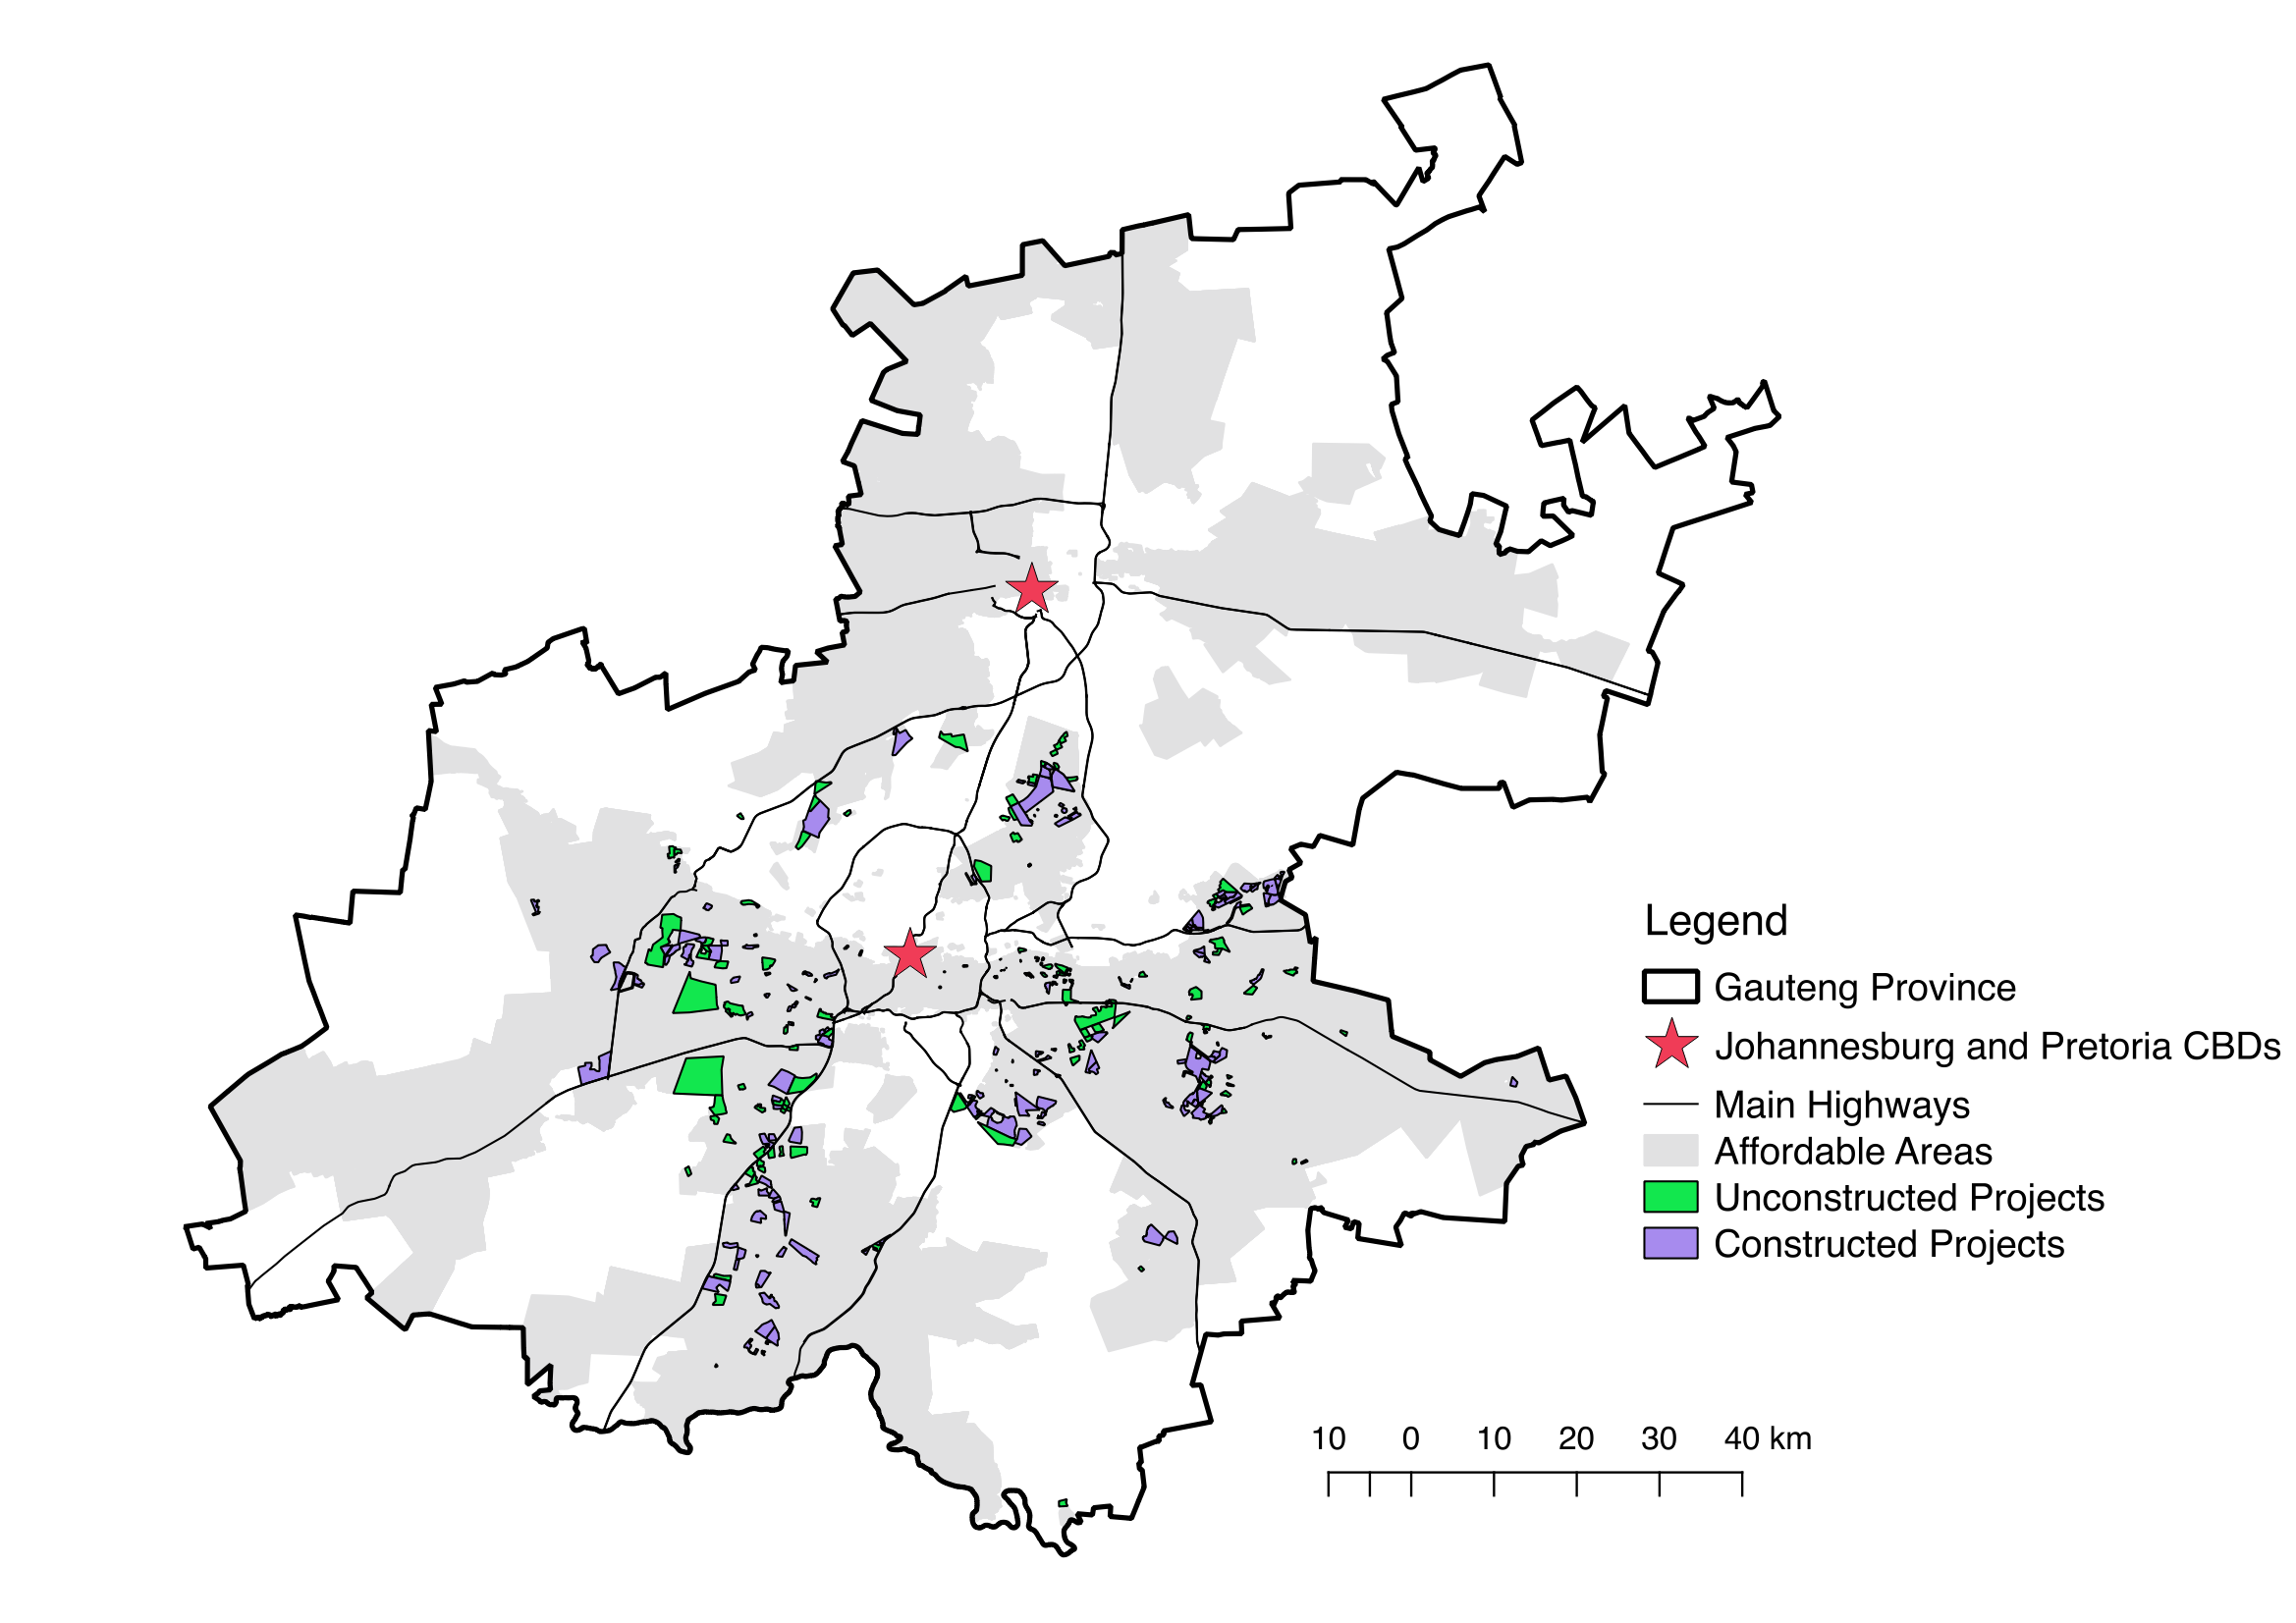
\includegraphics[scale=.6,trim={.9cm .4cm .9cm .4cm}]{figures/projmap_1.png}}
\end{figure}

Figure \ref{figure:map} maps the sample of constructed and unconstructed projects within the Gauteng province.  Projects are generally located far from central business districts, suggesting that inexpensive land plots are targeted by housing authorities.  Outside of the central business district, projects are distributed relatively evenly throughout the Johannesburg metro area.  Despite their distances from central business districts, projects are often next to arterial highways, potentially easing commuting costs for recipients.  Many constructed and unconstructed projects are adjacent to each other while others remain isolated.  

%   Since project construction often occurs in phases, 
%  which is consistent with revisions in project planning and 

% Since project construction often occurs in phases, adjacent constructed and unconstructed projects may indicate partial project completion.  In many other cases, constructed and unconstructed projects are isolated from each other.
% In some cases, constructed and unconstructed projects are adjacent to each other, possibly indicating authorities were unable to complete different phases of planned projects, In other cases, isolated projects of both types.  

% We note that our approach is not without limitations, and may introduce measurement error insofar as we are misattributing deeds to housing projects (false-positives), or assuming a project is unconstructed when it was actually constructed (false-negatives).  

% To provide some validation for our classification, we tabulate in Table~\ref{table:projectdescriptions} project descriptions from the 2008 administrative policy maps according to whether projects are classified as constructed or unconstructed by 2011.  As of 2008, we find that constructed projects are more likely to be classified as ``completed" or ``under implementation", while unconstructed projects are more likely to fall into ``proposed'' or ``planning'' categories.  Among constructed projects, we find 5 ``proposed'' and 8 ``planning'' indicators, which could imply either (1) these projects are false-positives or (2) while planned at some point prior to 2008, these projects were eventually completed by 2011.\footnote{We are unable to assess the frequency at which these descriptions are updated in the data.}  We also identify a single ``complete'' project as unconstructed, likely because its houses do not appear in our deeds records.  Figure \ref{fig:forchange} in section \ref{section:descriptives} further validates our sample, showing how formal housing increases disproportionately in projects classified as constructed. 


% According to the 1997 Housing Act, the South African Government defines adequate ``housing development'' as (1) ``permanent residential structures with secure tenure, ensuring internal and external privacy and providing adequate protection against the elements'' and (2) ``potable water, adequate sanitary facilities and domestic energy supply'' (\cite{housingact}).  

% To measure the spatial impacts of housing projects, we overlay 10 hm by 10 hm grids on all areas within 40 hm of housing projects.

To measure spatial impacts of housing projects similarly across multiple data sources, we overlay 0.01 sq km squares across all land within 4 km of projects.  We exclude plots where development is infeasible because they intersect with rivers, lakes, and/or mining excavation areas (10\% of total plots), which results in a total of 435,889 plots.  We then measure all spatial outcomes at the plot level. 

We measure local physical development by counting the number of houses, businesses, and public service buildings in each plot in 2001 and 2012.  We use hand-coded building data from 2001 and 2012 derived from high-resolution aerial and satellite imagery obtained through a partnership with GeoTerraImage (Pty) ltd., a local remote-sensing specialist.\footnote{\href{http://www.geoterraimage.com/}{\tt http://www.geoterraimage.com/}} The data classify buildings into 30 categories, including formal and informal houses. Informal houses are easily identified from their temporary nature, often made of materials such as recycled wood and corrugated metal. In contrast, formal houses are permanent, generally made out of brick and may have a pitched or a flat roof with tiles, zinc panels, or other materials.  The data also distinguish between non-backyard and backyard informal houses, which are often constructed on the same land plots as formal houses.  Beyond houses, we observe schools, health centers, water utility buildings, electricity buildings, and both formal and informal businesses.\footnote{Businesses are categorized as any ``commercial'' buildings and informal businesses are a subcategory labeled ``informal trading structures.''}  

% We construct outcome variables by counting the number of each type of building in each plot and year.


  % total houses split between formal houses and (3) informal residential structures, which we further decompose into backyard informal and non-backyard informal structures.  
% In Figure \ref{fig:bblumaps}, we provide an example of the raw data and a depiction of our griding procedure, using the 2012 data wave.

We measure demographic and housing characteristics with 2001 and 2011 Censuses of Population and Housing.  We average housing characteristics across households and demographic characteristics across people in each census block and year.  Gauteng is divided between 11,000 blocks in 2001 and 17,000 blocks in 2011, each containing 170 households on average.  We then attribute average census characteristics to each plot according to the census block with the greatest area of overlap.  We are able to match 355,721 plots to blocks in 2001 and 345,674 plots to blocks in 2011.  We also analyze the 1996 Census of Population and Housing matched to 362,178 plots in a robustness exercise.\footnote{\rv{In the census data, we identify informal housing as having one of three responses to the type of main dwelling question: (1) ``Informal dwelling (shack in backyard),'' (2) ``Informal dwelling (shack not in backyard, e.g. in an informal/squatter settlement or on a farm),'' and (3) ``House/flat/room in backyard.''  Formal housing includes all remaining categories.}}

\rv{To validate the remote-sensing building data, we find that the building measures of houses closely track the housing measures in the census.  We find a correlation between formal houses (building data) and households living in formal housing (census data) of 0.25 in 2001 and 0.30 in 2011.  In contrast, we find a correlation between informal houses (building data) and households living in informal housing (census data) of 0.79 in 2001 and 0.82 in 2011.}\footnote{\rv{Appendix Table~\ref{table:densitycorr} includes calculation details.}} \rv{  The stronger correlation for informal housing is consistent with informal structures often housing a single household and formal housing structures often including apartment buildings and duplexes that house many households.  In our later empirical results, we find similar estimates across census and building measures included in Appendix Table~\ref{table:census_ea_robust}.  }

\rv{Since it may be difficult to differentiate businesses and utility buildings from houses, we also validate the measures of businesses and public utilities.  We observe low correlations of these measures with employment and infrastructure access measures in the census.  Low correlations may be due to low numbers of people working near their homes, and public utilities locating on inexpensive land.  Informal businesses are negatively correlated with employment and income while overall businesses are positively correlated with employment and income.  This finding suggests that the measures are broadly associated with similar economic conditions.  We include measurement error as an important caveat in our later interpretations of results using these measures. }\footnote{\rv{Appendix Table~\ref{table:empcorr} provides correlations between businesses and informal businesses (building data) and employment and income (census).  Appendix Table~\ref{table:utilcorr} provides correlations between water utility and electricity buildings (building data) and piped water in the home and electric lighting (census).  }}  



To examine how projects affect nearby housing prices, we analyze deeds data covering the universe of \rv{formal} housing transactions from 2001 to 2011 in ``affordable areas,'' which are defined as census enumeration areas with 2010 mean house prices below R500,000.\footnote{These data were provided by the Affordable Land and Housing Data Centre, which tracks affordable housing markets.  The USD averaged around 7.70 Rands during the 2001-2011 period}  According to Figure~\ref{figure:map}, affordable areas contain nearly every project boundary.  Deeds include price, property location, property size, buyer name, and seller name.  Within project footprints, we find patterns consistent with the allocation of project houses to recipients: large numbers of properties are transferred in the same year at identical, low prices from sellers that are likely to be government housing authorities.\footnote{On average, constructed project footprints contain 316 transactions with seller names that contain ``government,'' ``municipality,'' ``city,'' or ``housing authority'' while unconstructed project footprints contain just 14.}  Since we are unable to precisely distinguish private sellers from government housing authorities within project footprints, we focus on property transactions that are located outside of project areas and are not sold by sellers with more than 30 transactions or whose names include ``government,'' ``municipality,'' ``city,'' or ``housing authority.''  We also exclude the top 1\% of prices as well as prices below 2,500 Rand, which are likely to be composed of mismeasured prices or titles exchanged between family members.  Following these criteria, our sample includes 247,131 deeds from 0 to 4 km from housing project footprints. 

\rv{Additional considerations may introduce measurement error into our price measure. Buyers and sellers may not have strong incentives to accurately report transaction prices on deeds records.  The timing of the transaction may also differ from the date that the deed is recorded.}

We attribute properties to plots according to the greatest area of overlap.  To match building and census observations from 2001 and 2011, we calculate average prices and number of transactions in each plot separately for transactions before 2006 (covering 21,330 plots) and after 2006 (covering 18,846 plots).  We also calculate averages for transactions before 2004 and after 2009, which may more closely reflect conditions in 2001 and 2011 respectively although reducing the sample size of transactions.







% We focus on properties located within 1.5 kilometers of constructed and unconstructed housing projects, forming a sample of over 62,000 transactions.  

% The deeds cover the universe of housing transactions from 2001 to 2011 in ``affordable areas,'' which are defined as census enumeration areas with 2010 mean house prices below R500,000.\footnote{These data were provided by the Affordable Land and Housing Data Centre, which tracks affordable housing markets.} Deeds include price, GPS location, plot size, buyer name, and seller name.  


% Although the data do not identify whether deeds belong to housing projects, we are able to infer project status according to whether the seller name includes a government or municipality when first transacted.  This project definition also excludes deeds flagged as large buildings used for commercial purposes (less than 2\% of transactions) as well as purchase prices more than R50,000 above the yearly nominal subsidy values (less than 4\% of remaining transactions), resulting in a sample of over 48,000 deeds.  Appendix Figure \ref{figure:transactionhist} plots the histogram of sale prices according to this project definition, finding substantial bunching around subsidy values for project deeds and a smooth distribution for non-project deeds.  We assign a completion date according to the modal year and month for deeds within each project.  Within projects, most government-sponsored properties are transacted in the same month.\footnote{Appendix \ref{appendix:histfreq} plots the distribution of subsidized and non-subsidized transactions around the modal transaction month.} 

% Though we observe responses from every surveyed household in both census waves, the data does not allow for linking households across time periods. 

% We analyze household-level responses describing the quality of their living quarters. 
% Our outcomes are mainly binary indicators and pertain to the household's access to services (flush toilets, water tap, electricity access), housing durability, and tenure arrangements. 
% We identify households 

% \subsection{Building Based Land Use}
% \label{section:data:bblu}


\section{Descriptive Statistics for Project Neighborhoods at Baseline}\label{section:descriptives}


\vspace{0mm}
\begin{table}[h!]
\centering
\caption{Average Characteristics per Plot before Project Construction}\label{table:projectdescriptives}
\vspace{0mm}
\resizebox{1\linewidth}{!}{
\begin{threeparttable}
\begin{tabular}{l*{1}{rrrrrrrrr}}
% \toprule
\\[-.5em]
% &\multicolumn{3}{c}{Constructed Projects} &\multicolumn{3}{c}{Unconstructed Projects}  \\[.5em] 
% Plot location& Inside & 0 - 10 hm  & 20 - 40 hm & Inside & 0 - 10 hm  & 20 - 40 hm \\[.3em]
&\multicolumn{3}{c}{Plots that } &\multicolumn{3}{c}{Plots outside of any project} &\multicolumn{3}{c}{Plots over 1 km from any project}  \\
&\multicolumn{3}{c}{overlap with} &\multicolumn{3}{c}{ but within 1 km of} &\multicolumn{3}{c}{but within 4 km of}  \\
\cmidrule(lr){2-4}\cmidrule(lr){5-7}\cmidrule(lr){8-10} 
Project types & Uncon & Con & Both & Uncon & Con & Both  & Uncon & Con & Both  \\ 
\\[-.5em]
Buildings \\ \midrule
\\[-.5em]
 \hspace{1em}Formal houses  & 0.79\,\,\,  & $2.50^{a}$  & 1.44\,\,\,  & 2.18\,\,\,  & $4.09^{a}$  & $4.63^{a}$  & 0.79\,\,\,  & 0.77\,\,\,  & $1.99^{a}$  \\[.15em] 
 \hspace{1em}Informal houses  & 1.97\,\,\,  & $8.04^{a}$  & $5.44^{a}$  & 1.31\,\,\,  & $3.21^{a}$  & $3.35^{a}$  & 0.02\,\,\,  & $0.26^{b}$  & $0.84^{a}$  \\[.15em] 
 \hspace{1em}Health centers  & 0.002\,\,\,  & 0.002\,\,\,  & $0.000^{b}$  & 0.016\,\,\,  & $0.004^{b}$  & 0.008\,\,\,  & 0.004\,\,\,  & 0.003\,\,\,  & 0.006\,\,\,  \\[.15em] 
 \hspace{1em}Schools  & 0.01\,\,\,  & $0.03^{a}$  & $0.00^{a}$  & 0.03\,\,\,  & $0.06^{a}$  & $0.06^{b}$  & 0.01\,\,\,  & 0.01\,\,\,  & $0.03^{a}$  \\[.15em] 
 \hspace{1em}Businesses  & 0.01\,\,\,  & $0.03^{c}$  & 0.02\,\,\,  & 0.06\,\,\,  & 0.07\,\,\,  & 0.05\,\,\,  & 0.06\,\,\,  & 0.04\,\,\,  & 0.08\,\,\,  \\[.15em] 
 \hspace{1em}Observations  & 19,148\,\,\,  & 23,488\,\,\,  & 588\,\,\,  & 43,816\,\,\,  & 45,157\,\,\,  & 14,079\,\,\,  & 96,369\,\,\,  & 73,636\,\,\,  & 114,311\,\,\,  \\[.15em] 

\\[-.5em]
Census Measures \\ \midrule
\\[-.5em]
 \hspace{1em}People  & 9.68\,\,\,  & $33.52^{a}$  & $21.97^{a}$  & 13.56\,\,\,  & $25.34^{a}$  & $25.86^{a}$  & 4.45\,\,\,  & 5.96\,\,\,  & $12.51^{a}$  \\[.15em] 
 \hspace{1em}Rooms per house  & 3.06\,\,\,  & 2.79\,\,\,  & 2.84\,\,\,  & 3.52\,\,\,  & 3.32\,\,\,  & 3.43\,\,\,  & 3.63\,\,\,  & 3.49\,\,\,  & 3.74\,\,\,  \\[.15em] 
 \hspace{1em}Owns house  & 0.27\,\,\,  & 0.32\,\,\,  & 0.30\,\,\,  & 0.36\,\,\,  & 0.39\,\,\,  & $0.41^{c}$  & 0.34\,\,\,  & 0.29\,\,\,  & 0.38\,\,\,  \\[.15em] 
 \hspace{1em}Electric lighting  & 0.54\,\,\,  & 0.54\,\,\,  & 0.52\,\,\,  & 0.69\,\,\,  & 0.69\,\,\,  & 0.69\,\,\,  & 0.75\,\,\,  & $0.60^{a}$  & 0.76\,\,\,  \\[.15em] 
 \hspace{1em}Flush toilet  & 0.55\,\,\,  & 0.59\,\,\,  & 0.56\,\,\,  & 0.72\,\,\,  & 0.72\,\,\,  & 0.73\,\,\,  & 0.70\,\,\,  & 0.61\,\,\,  & $0.78^{c}$  \\[.15em] 
 \hspace{1em}Piped water inside  & 0.33\,\,\,  & $0.21^{b}$  & 0.32\,\,\,  & 0.44\,\,\,  & $0.36^{a}$  & 0.41\,\,\,  & 0.46\,\,\,  & $0.34^{b}$  & 0.48\,\,\,  \\[.15em] 
 \hspace{1em}Is Employed  & 0.65\,\,\,  & $0.56^{b}$  & 0.63\,\,\,  & 0.71\,\,\,  & $0.64^{a}$  & $0.62^{a}$  & 0.80\,\,\,  & $0.76^{b}$  & $0.76^{b}$  \\[.15em] 
 \hspace{1em}Household income (R)  & 2,643\,\,\,  & $1,191^{b}$  & 1,785\,\,\,  & 2,784\,\,\,  & $1,879^{a}$  & $2,195^{b}$  & 4,060\,\,\,  & $2,624^{b}$  & 3,467\,\,\,  \\[.15em] 
 \hspace{1em}Observations  & 17,488\,\,\,  & 22,979\,\,\,  & 566\,\,\,  & 39,906\,\,\,  & 42,530\,\,\,  & 13,639\,\,\,  & 66,184\,\,\,  & 50,237\,\,\,  & 99,847\,\,\,  \\[.15em] 

\\[-.5em]
House Prices \\ \midrule
\\[-.5em]
 \hspace{1em}Price (Rand)  & & &  & 184,409\,\,\,  & $129,860^{a}$  & $130,628^{a}$  & 222,210\,\,\,  & 192,418\,\,\,  & $184,745^{c}$  \\[.15em] 
 \hspace{1em}Observations  & & &  & 3,112\,\,\,  & 4,986\,\,\,  & 1,528\,\,\,  & 2,066\,\,\,  & 2,069\,\,\,  & 7,514\,\,\,  \\[.15em] 

\\[-.5em]
Geographic Features\\ \midrule
\\[-.5em]
 \hspace{1em}Distance to CBD (km)  & 28.6\,\,\,  & $34.1^{a}$  & 28.7\,\,\,  & 29.3\,\,\,  & $34.4^{b}$  & 29.8\,\,\,  & 35.1\,\,\,  & 42.3\,\,\,  & $29.2^{c}$  \\[.15em] 
 \hspace{1em}Distance to Major Highway (km)  & 8.4\,\,\,  & 8.4\,\,\,  & 8.0\,\,\,  & 7.6\,\,\,  & 7.8\,\,\,  & 7.5\,\,\,  & 9.1\,\,\,  & 8.9\,\,\,  & $7.0^{b}$  \\[.15em] 
 \hspace{1em}Elevation (km)  & 1.61\,\,\,  & $1.58^{c}$  & 1.59\,\,\,  & 1.60\,\,\,  & 1.59\,\,\,  & 1.61\,\,\,  & 1.57\,\,\,  & 1.59\,\,\,  & $1.60^{c}$  \\[.15em] 
 \hspace{1em}Land Slope  & 0.13\,\,\,  & 0.08\,\,\,  & 0.13\,\,\,  & 0.16\,\,\,  & $0.08^{a}$  & 0.13\,\,\,  & 0.24\,\,\,  & 0.15\,\,\,  & 0.18\,\,\,  \\[.15em] 

% \\[-.3em]
%  Number of Projects & 140\,\,\, & 166\,\,\,  \\[.15em]   Average Project Area (ha) & 119\,\,\, & 118\,\,\,   \\[.15em]  
\bottomrule
\end{tabular}
\begin{tablenotes}
\item \footnotesize This table shows average measures for hectare plots grouped into 9 categories/columns: (1) plots that overlap with unconstructed projects only, (2) plots that overlap with constructed projects only, (3) plots that overlap with both types of projects, (4) plots with no project overlap and within 1 km of unconstructed projects only, (5) plots without overlap and within 1 km of constructed projects only, and (6) plots without overlap and within 1 km of both types of projects, (7) plots over 1 km from any project but within 4 km of only unconstructed projects, (8) plots over 1 km from any project but within 4 km of only constructed projects, and (9) plots over 1 km from any project but within 4 km of both types of projects.  These categories account for the fact that constructed and unconstructed projects are often clustered nearby each other as indicated by Figure~\ref{figure:map}.  T-tests are computed comparing plots near unconstructed projects (columns 1, 4, and 7) to plots near constructed projects (columns 2, 5, and 8) and also to plots near both projects (columns 3, 6, and 9) clustered at the project level and recorded with superscripts \textsuperscript{c} p$<$0.10,\textsuperscript{b} p$<$0.05,\textsuperscript{a} p$<$0.01 \,\, Building and census measures are from 2001, and house prices are from 2001 to 2004.  For reference, the USD averaged around 7.70 Rands during the 2001-2012 period.  
\end{tablenotes}
\end{threeparttable}
}
\end{table} 


% REDO

% We provide descriptive evidence on areas at baseline (before project construction) in Table~\ref{table:projectdescriptives} to evaluate possible counterfactuals for project construction.  


% Housing projects are located on relatively developed land plots (second column) within more developed neighborhoods (fifth column) compared to areas further from housing projects (eighth column) across measures of housing quality, public services, and infrastructure access.  These findings match qualitative evidence that policymakers prioritize locating projects on low-cost land nearby employment opportunities \citep{beninterview}.

% Areas inside constructed projects (second column) have higher densities of formal housing and much higher densities of informal housing and population than areas inside unconstructed projects (first column).  Many of these differences are statistically significant.  These findings are consistent with anecdotal evidence that policymakers prioritize some areas with dense preexisting slums for housing project implementation \citep{hofmeyr2008risk}.  Higher densities of formal housing in constructed project areas may indicate that parts of housing projects may have already been completed by 2001.  Constructed and unconstructed experience similar levels of infrastructure access and home quality (electric lighting, flush toilets, and piped water inside).  

% Areas nearby projects (0 - 40 hm) are more similar between constructed and unconstructed projects than areas within projects.  This finding may be partially driven by the fact that constructed and unconstructed projects are often clustered nearby each other as indicated in Figure~\ref{figure:map}.



\rv{We provide average plot characteristics before project construction in Table~\ref{table:projectdescriptives} to identify useful control groups for plots affected by project construction.  We observe large differences between plots near and far from projects.  We observe smaller, but still significant differences between plots near constructed projects and plots near unconstructed projects.  We conclude that plots near unconstructed projects provide useful yet imperfect controls for plots near constructed projects and that remaining differences between plots motivate a variety of robustness approaches in our empirical strategy.}

\rv{To examine differences between plots near and far from projects, we compare plots that overlap with project areas in columns 1-3 to plots outside but within 1 km of a project in columns 4-6.  We find that plots overlapping project areas generally have more informal housing, fewer health centers, schools, and businesses, and lower census development measures than plots outside but 1 km of a project.  Compared to overlapping plots, plots 1 to 4 km from projects have much less dense development while still better access to services and better census development measures.  These patterns match qualitative evidence that policymakers prioritize locating projects on low-cost land nearby employment opportunities \citep{bradlow2021weapons,bradlow2011housing}.}

\rv{To examine differences between constructed and unconstructed projects, we compare plots that overlap with unconstructed project areas (column 1) to plots that overlap with constructed project areas (column 2) and to the few plots that overlap with both project areas (column 3).  Plots that overlap with constructed projects or both projects have higher densities of formal housing and much higher densities of informal housing and population than plots that overlap with unconstructed projects.  These differences are statistically significant according to t-tests clustered at the project level.  Higher housing densities in constructed projects (before construction) may indicate that parts of housing projects may have already been completed by 2001.  This mismeasurement in the construction variable suggests that comparisons between constructed and unconstructed project areas would underestimate the total effect of project construction.}

\rv{Constructed and unconstructed project areas experience similar levels of infrastructure access and home quality (electric lighting, flush toilets, and piped water inside).  These census comparisons are mostly statistically insignificant.  These patterns suggest that policymakers may not have strongly prioritized project construction according to local levels of development.}








%%%% COMPARISON TESTER
% \vspace{0mm}
% \begin{table}[h!]
% \centering
% \caption{Average Characteristics per Plot before Project Construction1}\label{table:projectdescriptives1}
% \vspace{0mm}
% \resizebox{1\linewidth}{!}{
% \begin{threeparttable}
% \begin{tabular}{l*{1}{rrrrrrrrr}}
% % \toprule
% \\[-.5em]
% % &\multicolumn{3}{c}{Constructed Projects} &\multicolumn{3}{c}{Unconstructed Projects}  \\[.5em] 
% % Plot location& Inside & 0 - 10 hm  & 20 - 40 hm & Inside & 0 - 10 hm  & 20 - 40 hm \\[.3em]
% &\multicolumn{3}{c}{Plots that } &\multicolumn{3}{c}{Plots outside of any project} &\multicolumn{3}{c}{Plots over 1 km from any project}  \\
% &\multicolumn{3}{c}{overlap with} &\multicolumn{3}{c}{ but within 1 km of} &\multicolumn{3}{c}{but within 4 km of}  \\
% \cmidrule(lr){2-4}\cmidrule(lr){5-7}\cmidrule(lr){8-10} 
% Project types & Uncon & Con & Both & Uncon & Con & Both  & Uncon & Con & Both  \\ 
% \\[-.5em]
% Buildings \\ \midrule
% \\[-.5em]
%  \hspace{1em}Formal houses  & 0.58\,\,\,  & $2.50^{a}$  & $2.02^{c}$  & 2.06\,\,\,  & $4.52^{a}$  & $4.92^{a}$  & 0.88\,\,\,  & 0.70\,\,\,  & $2.07^{a}$  \\[.15em] 
 \hspace{1em}Informal houses  & 1.63\,\,\,  & $8.92^{a}$  & $5.30^{b}$  & 1.22\,\,\,  & $4.31^{a}$  & $3.32^{a}$  & 0.02\,\,\,  & $0.36^{c}$  & $0.80^{a}$  \\[.15em] 
 \hspace{1em}Health centers  & 0.003\,\,\,  & 0.003\,\,\,  & $0.000^{c}$  & 0.019\,\,\,  & $0.002^{b}$  & 0.012\,\,\,  & 0.004\,\,\,  & 0.002\,\,\,  & 0.007\,\,\,  \\[.15em] 
 \hspace{1em}Schools  & 0.01\,\,\,  & $0.03^{b}$  & 0.00\,\,\,  & 0.03\,\,\,  & $0.07^{a}$  & $0.06^{a}$  & 0.02\,\,\,  & 0.01\,\,\,  & $0.04^{a}$  \\[.15em] 
 \hspace{1em}Shops  & 0.02\,\,\,  & $0.03^{c}$  & 0.02\,\,\,  & 0.06\,\,\,  & 0.10\,\,\,  & 0.05\,\,\,  & 0.08\,\,\,  & 0.05\,\,\,  & 0.10\,\,\,  \\[.15em] 
 \hspace{1em}Observations  & 9,241\,\,\,  & 9,395\,\,\,  & 253\,\,\,  & 19,527\,\,\,  & 17,022\,\,\,  & 5,764\,\,\,  & 44,358\,\,\,  & 25,674\,\,\,  & 50,041\,\,\,  \\[.15em] 

% \\[-.5em]
% Census Measures \\ \midrule
% \\[-.5em]
%  \hspace{1em}People  & 7.71\,\,\,  & $37.79^{a}$  & $26.72^{a}$  & 12.37\,\,\,  & $29.76^{a}$  & $25.95^{a}$  & 4.61\,\,\,  & 6.81\,\,\,  & $12.62^{a}$  \\[.15em] 
 \hspace{1em}Rooms per house  & 3.08\,\,\,  & 2.63\,\,\,  & 2.99\,\,\,  & 3.37\,\,\,  & 3.11\,\,\,  & 3.44\,\,\,  & 3.50\,\,\,  & 3.15\,\,\,  & 3.64\,\,\,  \\[.15em] 
 \hspace{1em}Owns house  & 0.24\,\,\,  & 0.31\,\,\,  & 0.37\,\,\,  & 0.34\,\,\,  & 0.35\,\,\,  & $0.42^{b}$  & 0.33\,\,\,  & 0.24\,\,\,  & 0.38\,\,\,  \\[.15em] 
 \hspace{1em}Electric lighting  & 0.56\,\,\,  & 0.55\,\,\,  & 0.62\,\,\,  & 0.71\,\,\,  & 0.71\,\,\,  & 0.73\,\,\,  & 0.80\,\,\,  & $0.65^{b}$  & 0.81\,\,\,  \\[.15em] 
 \hspace{1em}Flush toilet  & 0.59\,\,\,  & 0.61\,\,\,  & 0.67\,\,\,  & 0.74\,\,\,  & 0.76\,\,\,  & 0.79\,\,\,  & 0.75\,\,\,  & 0.65\,\,\,  & 0.82\,\,\,  \\[.15em] 
 \hspace{1em}Piped water inside  & 0.35\,\,\,  & $0.22^{c}$  & 0.36\,\,\,  & 0.46\,\,\,  & $0.39^{c}$  & 0.45\,\,\,  & 0.50\,\,\,  & $0.38^{c}$  & 0.51\,\,\,  \\[.15em] 
 \hspace{1em}Is Employed  \hspace{1em}Household income (R)  & 3,026\,\,\,  & $1,347^{b}$  & 2,246\,\,\,  & 3,048\,\,\,  & $2,104^{b}$  & 2,688\,\,\,  & 4,746\,\,\,  & $3,058^{c}$  & 4,106\,\,\,  \\[.15em] 
 \hspace{1em}Observations  & 8,402\,\,\,  & 9,279\,\,\,  & 239\,\,\,  & 18,445\,\,\,  & 16,381\,\,\,  & 5,637\,\,\,  & 36,068\,\,\,  & 17,308\,\,\,  & 45,050\,\,\,  \\[.15em] 

% \\[-.5em]
% House Prices \\ \midrule
% \\[-.5em]
%  \hspace{1em}Price (Rand)  & & &  & 194,203\,\,\,  & $145,592^{b}$  & $142,097^{a}$  & 248,390\,\,\,  & 196,512\,\,\,  & 204,863\,\,\,  \\[.15em] 
 \hspace{1em}Observations  & & &  & 1,190\,\,\,  & 2,105\,\,\,  & 581\,\,\,  & 678\,\,\,  & 346\,\,\,  & 2,705\,\,\,  \\[.15em] 

% \\[-.5em]
% Geographic Features\\ \midrule
% \\[-.5em]
%  \hspace{1em}Distance to CBD (km)  & 28.6\,\,\,  & $34.1^{a}$  & 28.7\,\,\,  & 29.3\,\,\,  & $34.4^{b}$  & 29.8\,\,\,  & 35.1\,\,\,  & 42.3\,\,\,  & $29.2^{c}$  \\[.15em] 
 \hspace{1em}Distance to Major Highway (km)  & 8.4\,\,\,  & 8.4\,\,\,  & 8.0\,\,\,  & 7.6\,\,\,  & 7.8\,\,\,  & 7.5\,\,\,  & 9.1\,\,\,  & 8.9\,\,\,  & $7.0^{b}$  \\[.15em] 
 \hspace{1em}Elevation (km)  & 1.61\,\,\,  & $1.58^{c}$  & 1.59\,\,\,  & 1.60\,\,\,  & 1.59\,\,\,  & 1.61\,\,\,  & 1.57\,\,\,  & 1.59\,\,\,  & $1.60^{c}$  \\[.15em] 
 \hspace{1em}Land Slope  & 0.13\,\,\,  & 0.08\,\,\,  & 0.13\,\,\,  & 0.16\,\,\,  & $0.08^{a}$  & 0.13\,\,\,  & 0.24\,\,\,  & 0.15\,\,\,  & 0.18\,\,\,  \\[.15em] 

% % \\[-.3em]
% %  Number of Projects & 140\,\,\, & 166\,\,\,  \\[.15em]   Average Project Area (ha) & 119\,\,\, & 118\,\,\,   \\[.15em]  
% \bottomrule
% \end{tabular}
% \begin{tablenotes}
% \item \footnotesize REDO This table shows average measures for one-hectare plots grouped by their distance to the nearest constructed project and nearest unconstructed project.  Categories may overlap because constructed and unconstructed projects are sometimes clustered nearby each other as indicated by Figure~\ref{figure:map}.  Building and census measures are from 2001, and house prices are from 2001 to 2004.  \hmref  One hectare equals one $\text{hm}^{2}$.  For reference, the USD averaged around 7.70 Rands during the 2001-2012 period.  
% \end{tablenotes}
% \end{threeparttable}
% }
% \end{table} 





\section{Empirical Methodology}\label{section:methodology}


\begin{figure*}[hbtp]
    \caption{Measuring Spatial Exposure to \\ Example Housing Projects}
    \label{fig:spatialexposure}
    \centering
    \vspace{2mm}
    \begin{subfigure}[b]{.8\textwidth}
        \centering
        \caption[]{\small Plots overlapping with projects}  
        \vspace{-1mm}
        % 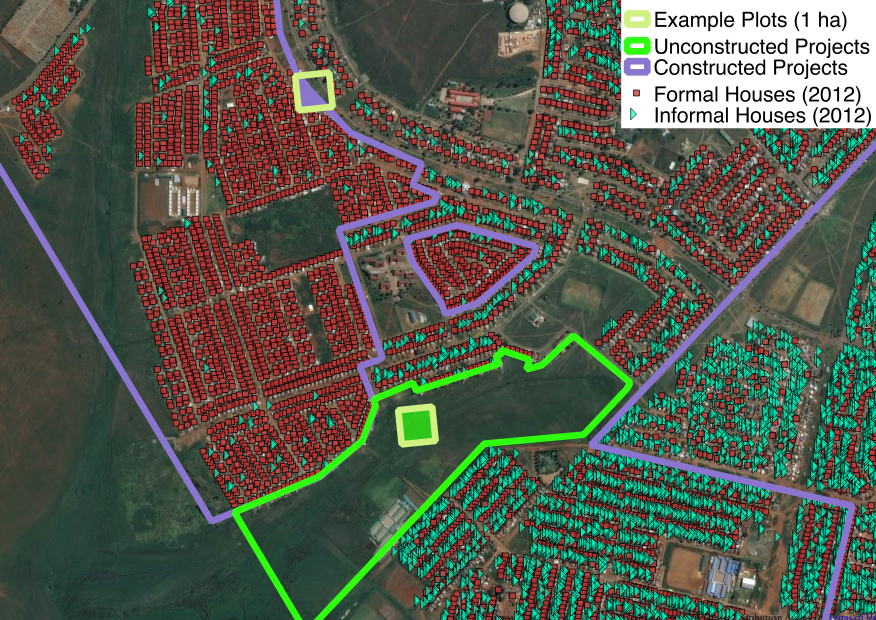
\includegraphics[width=\textwidth,trim={.2cm .2cm .2cm 0cm}, clip=true]{figures/hm_proj_75.png}
        % \label{fig:insideproj}

        \begin{tikzpicture}[  every node/.style={anchor=south west,inner sep=0pt}, x=1cm, y=1cm,]   
     \node (fig1) at (0,0)
       {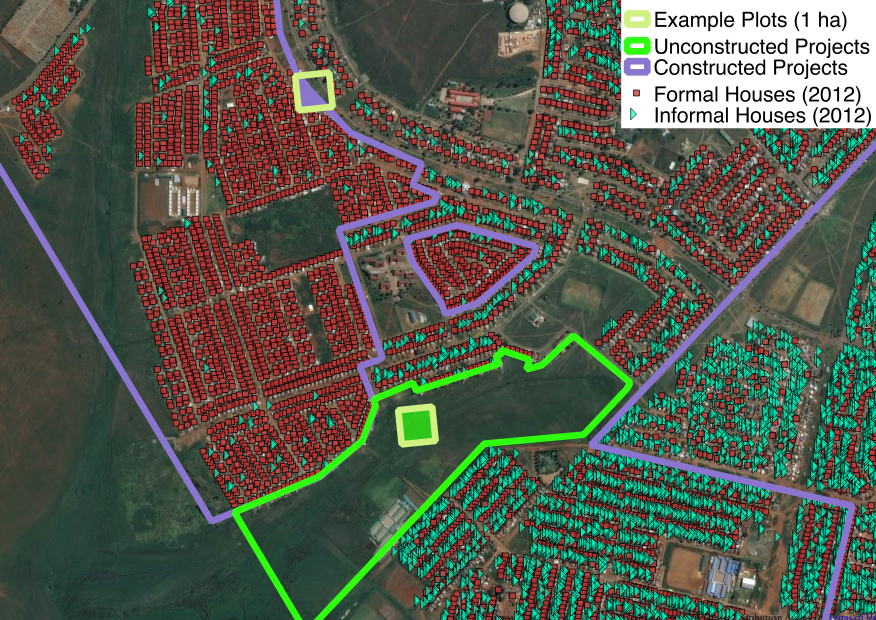
\includegraphics[width=\textwidth,trim={.2cm .2cm .2cm 0cm}, clip=true]{figures/hm_proj_75.png}};
		% \draw [line width=0.2mm,color=red,dashed] (1,2) -- (2,3);
		\node[font=\sffamily,align=left,text=white] at (5.2,7.6) {Plot A};
		\node[font=\sffamily,align=left,text=white] at (6.6,2.8) {Plot B};
		\end{tikzpicture}
\label{fig:insideproj}
    \end{subfigure}
    \vskip 1mm \vskip 0pt
    \begin{subfigure}[b]{.8\textwidth}  
        \centering 
        \caption[]{\small Plots outside of projects}
        \vspace{-1mm}

       \begin{tikzpicture}[  every node/.style={anchor=south west,inner sep=0pt}, x=1cm, y=1cm,]   
     \node (fig1) at (0,0)
       {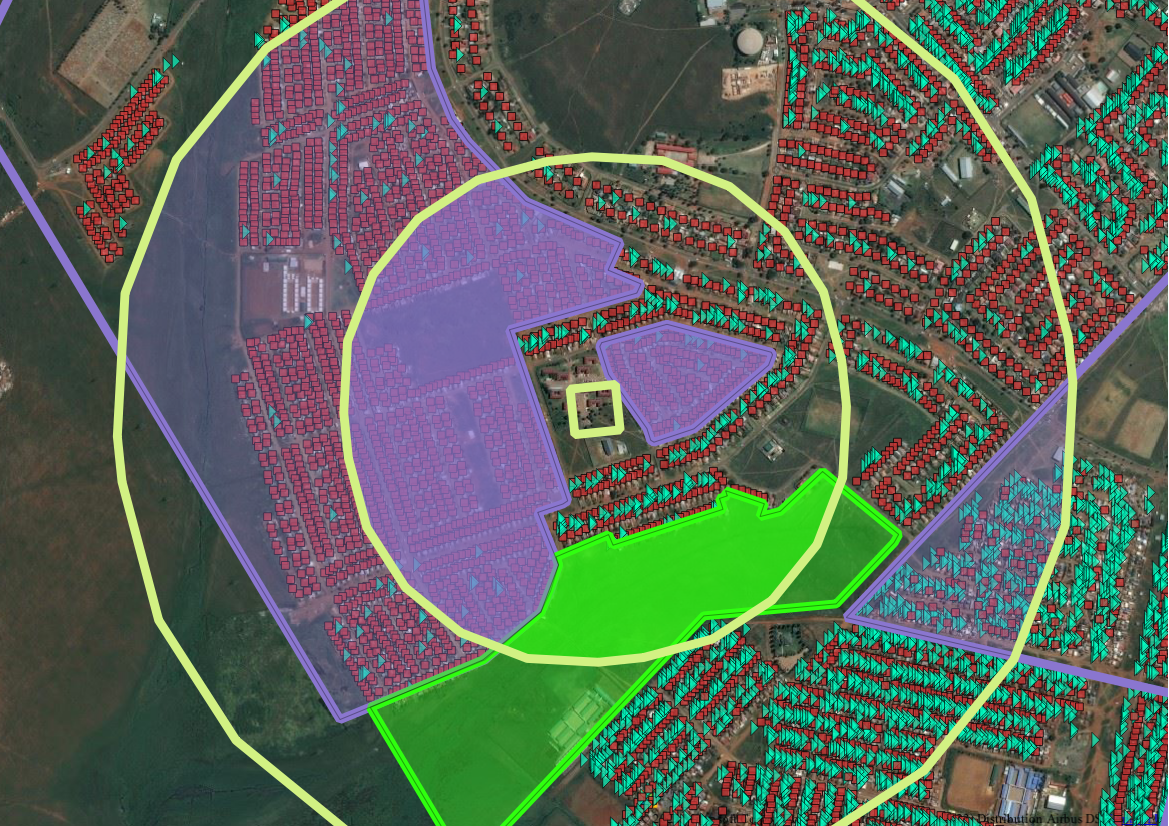
\includegraphics[width=\textwidth,trim={.2cm .2cm .2cm 0cm}, clip=true]{figures/newrings.png}};
		% \draw [line width=0.2mm,color=red,dashed] (1,2) -- (2,3);
		\node[font=\sffamily,align=left,text=white] at (2.3,7.1) {Ring 0.5 -- 1km};
		\node[font=\sffamily,align=left,text=white] at (4.5,5.8) {Ring 0 -- 0.5km};
		\end{tikzpicture}

        \label{fig:outsideproj}
    \end{subfigure}\\
    % {\footnotesize \hmrefha}
\end{figure*} 





To estimate project impacts, we compare changes in outcomes between constructed projects and planned but unconstructed projects.  We estimate both direct effects inside project footprints as well as spillover effects nearby project footprints.  To examine these effects when projects are clustered together and vary in size, we measure spatial exposure to place-based policies according to the extent to which each land plot's footprint and immediate neighborhoods overlap with project footprints.

\subsection{Measuring Spatial Exposure to Projects}\label{section:exposuremeasure}

Compared to the standard approach of measuring exposure in terms of the distance to the nearest project,\footnote{See \cite{diamond2019wants}, \cite{rossi2010housing}, and \cite{neumark2015place} for examples of the standard approach.} \rv{spatial overlap may work well in settings where projects are clustered together because overlap accounts for variation in the size, shape, and orientation of projects relative to each other.\footnote{\rv{This measure is similar to continuous exposure measures used in \cite{autor2014housing} and \cite{gechter2020spatial}.}}}  For example, a plot surrounded by many large projects may develop differently from a plot near one small project although both plots may share the same distance to their nearest project.  The map of projects in Figure~\ref{figure:map} indicates substantial variation in the layout of housing projects across space.  This overlap exposure measure also places greater weight on projects that cover larger land areas, which are also likely to reflect both larger government investments and larger changes to local neighborhoods.\footnote{This approach nests the intuition that housing projects may affect local economic outcomes by shifting neighborhood amenity values through changes in housing quality, composition of neighbors, and infrastructure quality.  In this setting, larger projects may produce greater shifts in these amenities, which in turn drive greater incentives to invest in these neighborhoods.  This approach may be less appropriate for place-based policies where households care mainly about their closest access point such as for schools or hospitals.}

\rv{For plots that overlap with project footprints, we measure direct exposure in terms of how much of each plot's area overlaps with project footprints.  We express this overlap as $\text{Area}\big(\textsc{Plot}  \cap  \textsc{Proj.}\big)$.  Figure~\ref{fig:insideproj} includes an example plot (``Plot A'') that overlaps with a constructed project as well as an example plot (``Plot B'') that overlaps with an unconstructed project.  Since Plot A only partially overlaps with a constructed project, its exposure lies between 0 and its total surface area, 0.01 sq km.  Plot B falls completely within an unconstructed project indicating exposure equal to 0.01 sq km. } 

\rv{For plots that do not overlap with project footprints, we measure spillover exposure by first, constructing 8 concentric rings 0.5 km wide around each plot and second, calculating how much of each ring's area overlaps with project footprints.  We express ring overlap as $\text{Area}\big(\textsc{Ring}^{k}  \cap  \textsc{Proj.}\big)$ where $k$ indexes rings from $0.5(k-1)$ to $0.5k$ km from plots.  Figure~\ref{fig:outsideproj} provides an example plot that falls just outside of project footprints but whose neighborhood rings from 0 to 0.5 km and from 0.5 to 1 km overlap with both constructed and unconstructed projects.  The exposure measure for each ring equals the area of overlap.}

% \rv{We then normalize our exposure measures so that one unit equals the overlap from one constructed project on average.  To normalize, we divide the measures by a constant equal to the overlap generated by an average constructed project.  In the second column of Table~\ref{table:spatialsummary}, the first row calculates that among plots that overlap projects, the average constructed project generates 0.007 sq km of overlap per plot.  We indicate normalized direct exposure as $\overline{\text{Area}}\big(\textsc{Plot}  \cap  \textsc{Proj.}\big)$, which equals $\frac{\text{Area}\big(\textsc{Plot}  \cap  \textsc{Proj.}\big)}{0.007}$.}

% \rv{In the last column of Table~\ref{table:spatialsummary}, the remaining rows indicate that for plots that do not overlap with projects, the average constructed project generates 0.093 sq km of overlap per 0-.5km ring and 0.236 sq km of overlap per 3.5-4km ring.  We indicate normalized spillover exposure as $\overline{\text{Area}}\big(\textsc{Ring}^{k}  \cap  \textsc{Proj.}\big)$, which equals $\frac{\text{Area}\big(\textsc{Ring}^{1}  \cap  \textsc{Proj.}\big)}{0.093}$ for $k=1$ and $\frac{\text{Area}\big(\textsc{Ring}^{8}  \cap  \textsc{Proj.}\big)}{0.236}$ for $k=8$.}

\rv{We then normalize our exposure measures so that one unit equals the overlap from one constructed project on average.  To normalize, we divide the measures by a constant equal to the overlap generated by an average constructed project.  The average constructed project overlaps at least partially with 150 plots.  Among these plots, the average constructed project generates 0.007 sq km of overlap per plot.  We indicate normalized direct exposure as $\overline{\text{Area}}\big(\textsc{Plot}  \cap  \textsc{Proj.}\big)$, which equals $\frac{\text{Area}\big(\textsc{Plot}  \cap  \textsc{Proj.}\big)}{0.007}$.}

\rv{Next, we consider exposure for rings around plots that do not share any overlap with projects.  The average constructed project overlaps with the 0-0.5 km rings of 302 plots.  Among these plots, the average overlap with 0-0.5 km rings is 0.093 sq km.  At the furthest distance, the average constructed project overlaps with the 3.5-4 km rings of 4,088 plots with average ring overlap of 0.236 sq km.  We indicate normalized spillover exposure as $\overline{\text{Area}}\big(\textsc{Ring}^{k}  \cap  \textsc{Proj.}\big)$, which equals $\frac{\text{Area}\big(\textsc{Ring}^{1}  \cap  \textsc{Proj.}\big)}{0.093}$ for $k=1$ and $\frac{\text{Area}\big(\textsc{Ring}^{8}  \cap  \textsc{Proj.}\big)}{0.236}$ for $k=8$.\footnote{For the remaining .5 km rings from 0.5 to 3.5 km, the average numbers of plot rings that overlap per project are 737, 1,268, 1,838, 2,410, 2,973, and 3,531 respectively.  Among these plots, the average areas of ring overlap in sq km are 0.193, 0.228, 0.237, 0.239, 0.238, and 0.237 respectively.}}



% The average overlap initially increases with ring diameter as rings cover larger surface areas.  Eventually, average overlap stabilizes for rings with wide diameters because these rings are often far away from projects.  

\rv{Because projects are clustered together, plot footprints and rings may overlap with multiple projects.  For example, Figure~\ref{fig:outsideproj} shows a plot where its ring from 0.5-1 km overlaps with two different constructed projects.  Similarly, plots near large projects may be exposed to multiple times the overlap area of an average project.  As a result, normalized exposure measures may have values greater than one.}


% The first two columns of Table~\ref{table:spatialsummary} show that the average unconstructed project overlaps with 142 plots and the average constructed project overlaps with 150 plots. The last two columns show that among overlapping plots, the average unconstructed project generates 0.006 sq km of overlap per plot.  Likewise, the average constructed project generates 0.007 sq km of overlap per plot. Since plots are defined to have 0.01 sq km of area, these figures indicate that many plots only partially overlap with projects.  

% The first two columns of Table~\ref{table:spatialsummary} show that the average unconstructed project overlaps with 276 rings 0-0.5km and 3,718 rings from 3.5-4km.  The average constructed project overlaps with 302 rings from 0-0.5km and 4,088 rings from 3.5-4km.  Projects have more overlap with further rings because further rings cover more surface area than nearer rings.  The last two columns show that for plots that do not overlap with projects, the average unconstructed project generates 0.088 sq km of overlap per 0-.5km ring and 0.219 sq km of overlap per 3.5-4km ring.  The average constructed project generates 0.093 sq km of overlap per 0-.5km ring and 0.236 sq km of overlap per 3.5-4km ring.  

 % plots and the average constructed project overlaps with 150 plots. The last two columns show that among overlapping plots, the average unconstructed project generates 0.006 sq km of overlap per plot.  Likewise, the average constructed project generates 0.007 sq km of overlap per plot. Since plots are defined to have 0.01 sq km of area, these figures indicate that many plots only partially overlap with projects. 
 


% \footnote{These figures can also be expressed as $\frac{1}{N_{Proj}}\sum_{k=1}^{N_{Proj}} \frac{1}{N^{k}_{Proj}} \sum_{l=1}^{N^{k}_{Plot}} \text{Area}\big(\textsc{Plot_l}  \cap  \textsc{Proj}_k\big)$ where $N_{Proj}$ indicates the total number of constructed or unconstructed projects.} 

% \footnote{These figures can also be expressed as $\frac{1}{N_{Proj}}\sum_{k=1}^{N_{Proj}} \sum_{l=1}^{N^{k}_{Plot}} \mathbbm{1}\big\{\text{Area}\big(\textsc{Plot_l}  \cap  \textsc{Proj}_k\big)>0\big\}$ where $N_{Proj}$ indicates the total number of constructed or unconstructed projects and $N^{k}_{Plot}$ is the number of plots near each project.} 

% On average across all plots, overlap between plots and projects equals 0.046 ha for constructed projects and 0.038 ha for unconstructed projects. Table~\ref{table:spatialsummary} summarizes this measure.


% \begin{table}
% \small
% \centering
% \caption{Average overlap generated per constructed project}\label{table:spatialsummary}
% \vspace{-2mm}
% % \resizebox{1\linewidth}{!}{
% \begin{threeparttable}
% \begin{tabular}{lGG}
% \toprule
%  % & Average count per project& Average overlap area (sq km) per project/plot  \\
%    & Average count per project& Average overlap area (sq km) per project/plot  \\
% \\[-.5em]
% % & Uncon & Con & Uncon & Con \\
% \midrule
%  Plot  & 150   & 0.007   \\[.15em] 
	
% \\[-.5em]
% Plot rings (km) \\
% that overlap with \\
% constructed projects \\
%  \hspace{1em}0-.5  & 302   & 0.093   \\[.15em] 
 \hspace{1em}.5-1  & 737   & 0.193   \\[.15em] 
 \hspace{1em}1-1.5  & 1,268   & 0.228   \\[.15em] 
 \hspace{1em}1.5-2  & 1,838   & 0.237   \\[.15em] 
 \hspace{1em}2-2.5  & 2,410   & 0.239   \\[.15em] 
 \hspace{1em}2.5-3  & 2,973   & 0.238   \\[.15em] 
 \hspace{1em}3-3.5  & 3,531   & 0.237   \\[.15em] 
 \hspace{1em}3.5-4  & 4,088   & 0.236   \\[.15em] 

% \bottomrule
% \end{tabular}
% \begin{tablenotes}
% \item \footnotesize  [REDO] DEF REDO TODAY PLEASE!!! This table shows the average hectares of overlap with housing projects for plots and rings around plots.  Overlap with rings around plots is only measured for plots that lie outside of project areas.  The sample includes plots within 40 hm of projects.  See Figure~\ref{fig:spatialexposure} for example rings around plots.
% \end{tablenotes}
% \end{threeparttable}
% % }
% \end{table}




% \begin{table}
% \small
% \centering
% \caption{Average overlap generated per project}\label{table:spatialsummary}
% \vspace{-2mm}
% % \resizebox{1\linewidth}{!}{
% \begin{threeparttable}
% \begin{tabular}{lrrrr}
% \toprule
%  & \multicolumn{2}{G}{Average number per project} & \multicolumn{2}{G}{Average overlap area (sq km) per project/plot}  \\
% \\[-.5em]
% & Uncon & Con & Uncon & Con \\
% \midrule
%  Plots with project overlap  & 142   & 150   & 0.006   & 0.007   \\[.15em] 
	
% \\[-.5em]
% Plot rings (km) \\
% with project overlap \\
%  \hspace{1em}0-.5  & 276   & 302   & 0.088   & 0.093   \\[.15em] 
 \hspace{1em}.5-1  & 681   & 737   & 0.177   & 0.193   \\[.15em] 
 \hspace{1em}1-1.5  & 1,172   & 1,268   & 0.205   & 0.228   \\[.15em] 
 \hspace{1em}1.5-2  & 1,681   & 1,838   & 0.214   & 0.237   \\[.15em] 
 \hspace{1em}2-2.5  & 2,192   & 2,410   & 0.216   & 0.239   \\[.15em] 
 \hspace{1em}2.5-3  & 2,696   & 2,973   & 0.217   & 0.238   \\[.15em] 
 \hspace{1em}3-3.5  & 3,205   & 3,531   & 0.218   & 0.237   \\[.15em] 
 \hspace{1em}3.5-4  & 3,718   & 4,088   & 0.219   & 0.236   \\[.15em] 

% \bottomrule
% \end{tabular}
% \begin{tablenotes}
% \item \footnotesize  [REDO] DEF REDO TODAY PLEASE!!! This table shows the average hectares of overlap with housing projects for plots and rings around plots.  Overlap with rings around plots is only measured for plots that lie outside of project areas.  The sample includes plots within 40 hm of projects. \hmref  See Figure~\ref{fig:spatialexposure} for example rings around plots.
% \end{tablenotes}
% \end{threeparttable}
% % }
% \end{table}







\subsection{Estimating Equations}\label{section:estimatingequations}

\rv{We estimate two differences-in-differences equations to recover the effects of direct and spillover exposure.  We estimate direct effects for plots that overlap with project footprints using the following expression}
\begin{align}
\label{eq:main1}
\begin{split}
\text{\textbf{Direct Effects}}& \\
Y_{it} \,=\, \alpha_0 \, + \,  &( \alpha_1 \, +  \, \alpha_2 \textsc{\small Post}_{t}) \, \times \,\overline{\text{Area}}\big(\textsc{Plot}_i  \cap  \textsc{Proj.}\big) \, + \\[.5em]
&( \alpha_3 \, +  \, \alpha_4 \textsc{\small Post}_{t})  \, \times \,  \overline{\text{Area}}\big(\textsc{Plot}_i \cap \textsc{Con. Proj.}\big) \, +\, \alpha_5 \, \textsc{Post}_t \, +\, \epsilon_{it}
\end{split}
\end{align}
\noindent \rv{where outcome $Y_{it}$ is measured for plot, $i$, and year, $t$. $\textsc{Post}_{t}$ equals one for 2012 and zero for 2001.  $\overline{\text{Area}}\big(\textsc{Plot}_i  \cap  \textsc{Proj.}\big)$ measures the sq km of overlap between plot $i$ and all project footprints while $\overline{\text{Area}}\big(\textsc{Plot}_i \cap \textsc{Con. Proj.}\big)$ measures the sq km of overlap between plot $i$ and only project footprints that are successfully constructed.  Both overlap measures are normalized by 0.007 km sq, which is the plot overlap generated by an average constructed project.  This normalization allows us to interpret our parameter of interest, $\alpha_4$, as the average effect of constructing a project on plots with at least some project overlap.}


   % Our parameter of interest, $\alpha_3$, measures the change in outcomes for plots overlapping with constructed projects relative to plots overlapping with planned but unconstructed projects.  
\rv{We estimate spillover effects for plots outside of project footprints using the following equation}
\begin{align}
\label{eq:main2}
\begin{split}
\text{\textbf{Spillover Effects}}& \\
Y_{it} \,=\, \beta_0 \,+\, \sum_{k=1}^{8} \, &(\beta_{1}^{k} \,+\, \beta_{2}^{k} \textsc{\small Post}_{t})  \, \times \, \overline{\text{Area}}\big(\textsc{Ring}_i^{k}  \cap  \textsc{Proj.}\big) \, + \\[.5em]
&(\beta_{3}^{k} \,+\, \beta_{4}^{k} \textsc{\small Post}_{t})  \, \times \,\overline{\text{Area}}\big(\textsc{Ring}_i^{k}  \cap \textsc{Con. Proj.}\big)\, + \, \beta_5 \textsc{\small Post}_{t} \, + \, \epsilon_{it} \\[.5em]
\end{split}
\end{align}
\noindent \rv{where $\overline{\text{Area}}\big(\textsc{Ring}_i^{k}  \cap  \textsc{Proj.}\big)$ measures the sq km of overlap between a ring from $0.5(k-1)$ to $0.5k$ km around plot $i$ and all project footprints.   $\overline{\text{Area}}\big(\textsc{Ring}_i^{k}  \cap  \textsc{Proj. Con.}\big)$ measures the sq km of overlap for this ring and only project footprints that are successfully constructed.  The overlap measures are normalized by the ring overlap generated by an average constructed project.  This normalization allows us to interpret each parameter of interest, $\beta_4^{k}$, as the average effect of constructing a project for plots whose $k$ ring has at least some project overlap.  We consider concentric 0.5 km concentric rings ranging from 0 to 4 km away from plots that implicitly assumes that any spillover effects dissipate by 4 km, which is consistent with recent literature on place-based policies.\footnote{\cite{diamond2019wants} and \cite{rossi2010housing} find that main effects are concentrated within 1 km of place-based policies.}   For reference, Figure~\ref{fig:spatialexposure} includes an example of rings from 0 to 0.5 km and 0.5 to 1 km.}

\rv{Standard errors are clustered at the project-level with projects assigned to each plot according to the greatest area of overlap first with the plot's footprint and if no overlap, then with the closest overlapping ring.  We also correct standard errors for multiple hypothesis testing using the Bonferroni method and test robustness to spatially correlated errors.}

Our coefficients of interest --- $\alpha_4$ for the direct effect and $\beta_4^{k}$ for the spillover effects --- capture the causal effects of project construction under the assumption that in the absence of project construction, plots exposed to constructed project footprints would have evolved in the same way as plots exposed to unconstructed project footprints.  Our flexible specification of spillover effects from 0 to 4 km allows us to examine how these effects dissipate across space.  We hypothesize that spillover effects are likely to be concentrated in nearby neighborhoods.  This specification also provides a partial test for whether areas with constructed projects and areas with unconstructed projects are likely to follow parallel trends.  We hypothesize that spillover effects are likely to dissipate at further distances (ie. 2 to 4 km).  Therefore, evidence of effects at these distances may suggest that areas with constructed projects develop differently from areas with unconstructed projects for reasons unrelated to project construction.  For example, housing projects may be accompanied by broader urban renewal programs that affect broader areas around projects.  Alternatively, policymakers may prioritize growing areas for project construction.

By comparing changes over time, this approach accounts for baseline differences between constructed and unconstructed project areas.  This approach also controls for aggregate factors that affect development in the metro-area by examining differential changes between constructed and unconstructed project areas.  

This framework does not allow for trends that are also correlated with whether projects are constructed.  For example, forward-looking households may anticipate project construction and alter their housing investment decisions accordingly.  Qualitative evidence suggests that it would be difficult for households to anticipate construction in this context due to substantial uncertainty in project location and timing.  Project managers face difficulties coordinating stakeholders and sourcing funding while housing authorities are rarely transparent about project planning \citep{serihistory}.\footnote{\cite{diamond2019wants} also leverage uncertainty in project timing to study affordable housing in the US.} 

Our approach assumes that project construction occurs between 2001 and 2012.  To the extent that some parts of projects may have been constructed before 2001, our estimates of the effects of project construction would be biased toward zero, suggesting that our approach may underestimate the full effects.


%%%%%%%%% %%%%%%%%%%%%%%%%%% %%%%%%%%%%%%


\section{Estimation Results}\label{section:results}

\rv{We first use our estimation strategy to measure housing project construction, consisting of new formal houses, people living in these houses, and infrastructure services to support the projects.  We then estimate effects of project construction within project footprints, including informal housing and people living in informal housing.  Finally, we estimate spillover effects of project construction on plots just outside of project footprints.  We consider spillover effects on demographics, infrastructure, and both formal and informal housing.}

\subsection{Measuring Housing Project Construction}\label{section:measuringprojects}

\rv{We measure housing construction by estimating equation (\ref{eq:main1}) for plots overlapping with project footprints.  We consider variables that measure formal houses, people living in these houses, and infrastructure built to support the projects.  }

\rv{We observe that project construction leads to massive increases in the number of formal houses and people living in formal houses.  Table~\ref{table:main_formal_proj} includes the difference-in-differences coefficients for these outcomes.  Project construction is associated with 4.4 more formal houses and 20.4 more people for plots that overlap with projects.  These increases are statistically significant at the 1\% level and economically large when compared with pre-construction averages.  Given that the average constructed project overlaps with 150 plots, the estimates suggest that each project leads to 660 new formal houses and 3,060 new people living in formal houses.  These results indicate that constructed housing projects generate large-scale growth in local populations compared to similar but unconstructed project areas.}

\begin{table}[h!]
\small
\centering
\caption{Direct Effects on Formal Housing and Inhabitants}\label{table:main_formal_proj}
\vspace{-2mm}
% \resizebox{1\linewidth}{!}{
\begin{threeparttable}
\begin{tabular}{lCC}
\toprule
                    &(1)&(2)\\[.5em] &Formal Houses                   &People in Formal Houses \\ \midrule                    \\
Post $\times$ Const.&        4.43\textsuperscript{a}&       20.37\textsuperscript{a}\\
                    &      (0.54)                   &      (1.85)                   \\
                    &      [0.00]                   &      [0.00]                   \\
Mean Pre            &        1.73                   &        9.49                   \\
Mean Post           &        5.65                   &       27.29                   \\
R$^2$               &       0.178                   &       0.223                   \\
N                   &      86,448                   &      79,688                   \\

\bottomrule
\end{tabular}
\begin{tablenotes}
\item \footnotesize 
This table provides the differences-in-difference coefficient for how housing construction affects the total number of formal houses and people living in formal houses for plots that overlap with projects. Houses are measured from the building data and population is measured from census data.  Population has fewer observations because census enumerator areas do not intersect with every plot. \regtextfirst
\end{tablenotes}
\end{threeparttable}
% }
\end{table}

\rv{Next, we document that projects may directly improve the quality of neighborhoods by introducing well-serviced houses.  Table~\ref{table:census_formal_proj} reports impacts on census outcomes.  Columns (1) to (5) indicate that formal houses in constructed projects appear to be larger with better services than formal houses in unconstructed project footprints after project construction; however, most of these differences are statistically insignificant.  Columns (6) to (10) indicate that the demographics of people living in formal houses change similarly in constructed and unconstructed projects.}


\begin{table}[h!]
\small
\centering
\caption{Direct Effects on Formal Housing Quality and Inhabitant Demographics}\label{table:census_formal_proj}
\vspace{-2mm}
% \resizebox{1\linewidth}{!}{
\begin{threeparttable}
\begin{tabular}{lCCCCC}
\toprule
                    &(1)&(2)&(3)&(4)&(5)\\[.5em] &Total Rooms                   &   Own House                   &Electric Lighting                   &Flush Toilet                   &Piped Water Inside\\ \midrule                    \\
Post $\times$ Const.&        0.25                   &        0.04                   &        0.02                   &        0.10                   &        0.13\textsuperscript{a}\\
                    &      (0.20)                   &      (0.04)                   &      (0.04)                   &      (0.07)                   &      (0.04)                   \\
                    &      [0.62]                   &      [0.62]                   &      [0.62]                   &      [0.53]                   &      [0.00]                   \\
Mean Pre            &        3.45                   &        0.37                   &        0.65                   &        0.67                   &        0.34                   \\
Mean Post           &        3.75                   &        0.36                   &        0.76                   &        0.81                   &        0.56                   \\
R$^2$               &       0.034                   &       0.033                   &       0.030                   &       0.078                   &       0.124                   \\
N                   &      78,510                   &      78,611                   &      78,611                   &      78,611                   &      78,611                   \\

\\
\\\midrule
                    &(6)&(7)&(8)&(9)&(10)\\[.5em] &Age                   &     African                   &Household Size                   &  Employment                   &Log Income \\ \midrule                    \\
Post $\times$ Const.&       -1.09                   &       -0.02                   &        0.30                   &        0.05                   &       -0.08                   \\
                    &      (0.84)                   &      (0.03)                   &      (0.15)                   &      (0.03)                   &      (0.15)                   \\
                    &      [0.58]                   &      [1.00]                   &      [0.20]                   &      [0.20]                   &      [1.00]                   \\
Mean Pre            &       41.03                   &        0.82                   &        3.42                   &        0.74                   &        7.27                   \\
Mean Post           &       42.52                   &        0.90                   &        3.05                   &        0.79                   &        8.03                   \\
R$^2$               &       0.030                   &       0.111                   &       0.108                   &       0.074                   &       0.300                   \\
N                   &      78,584                   &      78,611                   &      78,610                   &      77,953                   &      77,699                   \\

\bottomrule
\end{tabular}
\begin{tablenotes}
\item \footnotesize This table shows difference-in-differences coefficients for census measures of people living in formal houses.  The estimates are for plots that overlap with projects. Age, African, and employment are measured for the household head.  Employment is calculated for heads of household between ages 18 to 65.  Log income is measured at the household level.   \regtextfirst The Bonferroni correction is computed separately for columns 1-5 and columns 6-10.
\end{tablenotes}
\end{threeparttable}
% }
\end{table}

\rv{Table~\ref{table:infra_proj} tests whether housing projects appear to be accompanied by broader infrastructure investments.  Columns (1) and (3) indicate that projects substantially increase the number of water utility buildings and health centers in their footprints.  Columns (2) and (4) find little effect on electricity utility buildings and schools.}

\rv{Taken together, these results suggest that while projects build a substantial amount of housing and infrastructure, the resulting house quality and recipient demographics are largely similar to formal housing in unconstructed project areas.  We also note that measurement error from interpolating census data to the plot-level may prevent our approach from precisely identifying effects.}

% Maybe ADD THIS LATER?! Coefficients for the interaction of Post with plot overlap indicate that unconstructed project areas experience positive changes within their footprints even in the absence of project construction, which is consistent with investment crowding into these relatively undeveloped areas.  Yet, changes for unconstructed projects are at least 3 times smaller than for constructed projects, reiterating the substantial size of project investments.  Small and largely insignificant coefficients for the interaction of Post with 0 to 5 hm ring overlap suggest that unconstructed projects are not associated with nearby spillover changes. 
\begin{table}[h!]
\small
\centering
\caption{Infrastructure Investments}\label{table:infra_proj}
\vspace{-2mm}
% \resizebox{1\linewidth}{!}{
\begin{threeparttable}
\begin{tabular}{lCCCC}
\toprule
                    &(1)&(2)&(3)&(4)\\[.5em] &Water Utility Buildings                   &Electricity Utility Buildings                   &Health Centers                   &Schools \\ \midrule                    \\
Post $\times$ Const.&      0.0164\textsuperscript{a}&      0.0004                   &      0.0007\textsuperscript{b}&      0.0418\textsuperscript{a}\\
                    &    (0.0036)                   &    (0.0003)                   &    (0.0003)                   &    (0.0097)                   \\
                    &    [0.0000]                   &    [0.2376]                   &    [0.0461]                   &    [0.0001]                   \\
Mean Pre            &      0.0128                   &      0.0022                   &      0.0018                   &      0.0235                   \\
Mean Post           &      0.0296                   &      0.0034                   &      0.0025                   &      0.0710                   \\
R$^2$               &       0.005                   &       0.000                   &       0.001                   &       0.003                   \\
N                   &      86,448                   &      86,448                   &      86,448                   &      86,448                   \\

\bottomrule
\end{tabular}
\begin{tablenotes}
\item \footnotesize This table shows difference-in-differences coefficients for building measures of infrastructure investments for plots that overlap with projects.
 \regtextfirst
\end{tablenotes}
\end{threeparttable}
% }
\end{table}


\subsection{Estimating Effects Within Project Footprints}\label{section:directeffects}

\rv{We estimate project effects on informal housing and people living informal housing within project footprints using equation (\ref{eq:main1}).  Table~\ref{table:main_informal_proj} includes difference-in-differences estimates for plots that overlap with project footprints.  According to column (1), projects lead to an overall increase in informal housing equal to 1.7 houses per plot, which is statistically significant at the 5\% level. }

\begin{table}[h!]
\small
\centering
\caption{Direct Effects on Informal Housing and Inhabitants}\label{table:main_informal_proj}
\vspace{-2mm}
% \resizebox{1\linewidth}{!}{
\begin{threeparttable}
\begin{tabular}{lCCCC}
\toprule
                    &(1)&(2)&(3)&(4)\\[.5em] &Informal Houses                   &Informal Backyard Houses                    &Informal Non-Backyard Houses                    &People living in Informal Housing\\ \midrule                   \\
Post $\times$ Const.&        1.65\textsuperscript{b}&        4.44\textsuperscript{a}&       -2.80\textsuperscript{a}&       -3.70\textsuperscript{b}\\
                    &      (0.69)                   &      (0.77)                   &      (0.61)                   &      (1.82)                   \\
                    &      [0.04]                   &      [0.00]                   &      [0.00]                   &      [0.04]                   \\
Mean Pre            &        5.31                   &        0.52                   &        4.80                   &       13.59                   \\
Mean Post           &        8.57                   &        4.42                   &        4.15                   &       13.96                   \\
R$^2$               &       0.084                   &       0.166                   &       0.036                   &       0.051                   \\
N                   &      86,448                   &      86,448                   &      86,448                   &      79,688                   \\

\bottomrule
\end{tabular}
\begin{tablenotes}
\item \footnotesize 
 This table shows difference-in-differences coefficients for census measures of people living in informal houses.  The estimates are for plots that overlap with projects. Age, African, and employment are measured for the household head.  Employment is calculated for heads of household between ages 18 to 65.  Log income is measured at the household level. Population has fewer observations because census enumerator areas do not intersect with every plot.   \regtextfirst
\end{tablenotes}
\end{threeparttable}
% }
\end{table}

\rv{Columns (2) and (3) disaggregate the total effect into effects on informal backyard houses and informal non-backyard houses.  Backyard housing is a common phenomenon in South Africa where households erect informal dwellings within the plots of formal dwellings \citep{Brueckner2018backyarding}.  We observe a large increase in backyard housing at the same magnitude as the increase in formal housing in Table~\ref{table:main_formal_proj}.  This finding suggests that almost every formal project house is accompanied by an informal, backyard house constructed on the same parcel of land.  We also estimate a relative decline in informal, non-backyard houses in constructed project areas relative to unconstructed project areas.  The number of people living in informal housing declines as a result of project construction.  These findings are consistent with larger non-backyard houses being replaced by smaller backyard houses.}
% consistent with qualitative evidence that housing authorities cleared preexisting slums before constructing new projects \citep{hofmeyr2008risk}. 

\rv{Estimates in Table~\ref{table:census_informal_proj} show how project construction affects the quality of informal housing as well as the demographics of people living in these houses.  Columns (1) to (5) indicate that while informal houses may become smaller after project construction, they have much better access to services including flush toilets and piped water.  One possible explanation is that people in formal houses are able to share their services like flush toilets and piped water with people living in their backyards.  Columns (6) to (10) find no effects on the demographics of people living in informal housing.}

\begin{table}[h!]
\small
\centering
\caption{Direct Effects on Informal House Quality and Demographics for Inhabitants}\label{table:census_informal_proj} 
\vspace{-2mm}
% \resizebox{1\linewidth}{!}{
\begin{threeparttable}
\begin{tabular}{lCCCCC}
\toprule
                    &(1)&(2)&(3)&(4)&(5)\\[.5em] &Total Rooms                   &   Own House                   &Electric Lighting                   &Flush Toilet                   &Piped Water Inside\\ \midrule                    \\
Post $\times$ Const.&       -0.11                   &       -0.05                   &        0.11                   &        0.17\textsuperscript{a}&        0.15\textsuperscript{a}\\
                    &      (0.09)                   &      (0.03)                   &      (0.06)                   &      (0.05)                   &      (0.04)                   \\
                    &      [0.22]                   &      [0.13]                   &      [0.12]                   &      [0.00]                   &      [0.00]                   \\
Mean Pre            &        2.06                   &        0.19                   &        0.41                   &        0.45                   &        0.15                   \\
Mean Post           &        2.22                   &        0.19                   &        0.62                   &        0.60                   &        0.28                   \\
R$^2$               &       0.024                   &       0.022                   &       0.094                   &       0.109                   &       0.078                   \\
N                   &      74,461                   &      74,461                   &      74,461                   &      74,461                   &      74,461                   \\

\\
\\\midrule
                    &(6)&(7)&(8)&(9)&(10)\\[.5em] &Age                   &     African                   &Household Size                   &  Employment                   &Log Income \\ \midrule                    \\
Post $\times$ Const.&       -0.71                   &       -0.01                   &       -0.07                   &        0.01                   &       -0.08                   \\
                    &      (0.63)                   &      (0.01)                   &      (0.11)                   &      (0.03)                   &      (0.07)                   \\
                    &      [1.00]                   &      [1.00]                   &      [1.00]                   &      [1.00]                   &      [1.00]                   \\
Mean Pre            &       38.64                   &        0.94                   &        2.83                   &        0.66                   &        6.80                   \\
Mean Post           &       37.61                   &        0.97                   &        2.53                   &        0.80                   &        7.66                   \\
R$^2$               &       0.018                   &       0.033                   &       0.066                   &       0.121                   &       0.356                   \\
N                   &      74,461                   &      74,461                   &      74,461                   &      73,670                   &      73,433                   \\

\bottomrule
\end{tabular}
\begin{tablenotes}
\item \footnotesize This table shows the difference-in-differences coefficients for census measures of people living in informal houses. Age, African, and employment are measured for the household head.  Employment is calculated for heads of household between ages 18 to 65.  Log income is measured at the household level.  Employment and log-income are not available for all plots.   \regtextfirst The Bonferroni correction is computed separately for columns 1-5 and columns 6-10.
\end{tablenotes}
\end{threeparttable}
% }
\end{table}


\rv{We also examine whether projects invite business development in their footprints.  The building data record total businesses and a subcategory identified as informal businesses although there may be some imprecision in categorizing businesses in this dataset as discussed in Section~\ref{section:data}.  Table~\ref{table:agglom_proj} finds large, statistically significant increases in total businesses, which are driven in large part by informal businesses.  The point estimate for informal businesses is almost four times the pre period mean.  These findings are consistent with housing recipients using their new dwellings as opportunities to launch their own businesses.  An important caveat is that since the building data is mainly derived from aerial imagery, there may be substantial scope for mismeasurement if backyard housing and informal businesses have similar visual markers.}

\begin{table}[h!]
\small
\centering
\caption{Direct Effects on Economic Outcomes}\label{table:agglom_proj}
\vspace{-2mm}
% \resizebox{1\linewidth}{!}{
\begin{threeparttable}
\begin{tabular}{lCC}
\toprule
                    &(1)&(2)\\[.5em] &Businesses                   &Informal Businesses\\ \midrule                    \\
Post $\times$ Const.&       0.036\textsuperscript{a}&       0.023\textsuperscript{a}\\
                    &     (0.008)                   &     (0.006)                   \\
                    &     [0.000]                   &     [0.000]                   \\
Mean Pre            &       0.021                   &       0.006                   \\
Mean Post           &       0.059                   &       0.028                   \\
R$^2$               &       0.005                   &       0.003                   \\
N                   &      86,448                   &      86,448                   \\

\bottomrule
\end{tabular}
\begin{tablenotes}
\item \footnotesize 
This table shows the difference-in-differences estimates for average business counts per plot from the business data.  The estimates are for plots that overlap with projects. \regtextfirst
\end{tablenotes}
\end{threeparttable}
% }
\end{table}



\subsection{Spillover Effects}\label{section:spillovereffects}

\rv{We estimate spillover effects on plots nearby project footprints using equation (\ref{eq:main2}).  Table~\ref{table:main_spill} provides spillover difference-in-differences estimates on quantities of formal houses, informal houses, and people living in these houses.  The table includes the difference-in-differences coefficients after project construction for exposure to constructed projects given by $\beta_4^{k}$ (k=1,..,8) in equation (\ref{eq:main2}).  Appendix Tables~\ref{table:main_full} and \ref{table:main_full2} include the full set of coefficients.   }

\begin{table}[h!]
\small
\centering
\caption{Spillover Effects on Population and Informal Housing}\label{table:main_spill}
\vspace{-2mm}
\resizebox{1\linewidth}{!}{
\begin{threeparttable}
\begin{tabular}{lCCCCC}
\toprule
                    &(1)&(2)&(3)&(4)&(5)\\[.5em] &Formal Houses                    &People in Formal Houses                   &Informal Backyard Houses                   &Informal Non-Backyard Houses                   &People in Informal Houses \\ \midrule                    \\
Post $\times$ Const. $\times$ \\
 \hspace{1.5em}Ring (km) \\[1em] \hspace{2.5em} 0 - .5&        0.22\textsuperscript{b}&        1.33\textsuperscript{a}&        0.34\textsuperscript{a}&        0.09                   &        0.57                   \\
                    &      (0.10)                   &      (0.48)                   &      (0.12)                   &      (0.15)                   &      (0.42)                   \\[0.3em]
\hspace{2.5em} .5 - 1&        0.07                   &        0.73\textsuperscript{c}&        0.01                   &       -0.20\textsuperscript{c}&       -0.93\textsuperscript{a}\\
                    &      (0.09)                   &      (0.43)                   &      (0.11)                   &      (0.11)                   &      (0.32)                   \\[0.3em]
\hspace{2.5em} 1 - 1.5&       -0.10\textsuperscript{c}&       -0.57                   &        0.03                   &        0.10                   &        0.45                   \\
                    &      (0.05)                   &      (0.35)                   &      (0.10)                   &      (0.07)                   &      (0.31)                   \\[0.3em]
\hspace{2.5em} 1.5 - 2&        0.02                   &        0.38                   &        0.04                   &       -0.03                   &       -0.02                   \\
                    &      (0.05)                   &      (0.27)                   &      (0.07)                   &      (0.06)                   &      (0.25)                   \\[0.3em]
\hspace{2.5em} 2 - 2.5&        0.04                   &       -0.13                   &        0.09                   &        0.01                   &        0.10                   \\
                    &      (0.05)                   &      (0.24)                   &      (0.06)                   &      (0.04)                   &      (0.17)                   \\[0.3em]
\hspace{2.5em} 2.5 - 3&       -0.01                   &        0.36\textsuperscript{c}&        0.03                   &       -0.02                   &       -0.11                   \\
                    &      (0.03)                   &      (0.21)                   &      (0.05)                   &      (0.04)                   &      (0.16)                   \\[0.3em]
\hspace{2.5em} 3 - 3.5&       -0.01                   &       -0.01                   &        0.02                   &        0.05                   &        0.04                   \\
                    &      (0.03)                   &      (0.21)                   &      (0.05)                   &      (0.04)                   &      (0.15)                   \\[0.3em]
\hspace{2.5em} 3.5 - 4&       -0.02                   &       -0.12                   &        0.02                   &        0.01                   &        0.05                   \\
                    &      (0.03)                   &      (0.18)                   &      (0.04)                   &      (0.03)                   &      (0.10)                   \\[0.3em]
Mean Pre            &        1.81                   &        9.52                   &        0.52                   &        0.41                   &        2.61                   \\
Mean Post           &        2.06                   &       12.87                   &        1.20                   &        0.52                   &        2.83                   \\
R$^2$               &       0.049                   &       0.040                   &       0.046                   &       0.009                   &       0.016                   \\
N                   &     785,330                   &     621,707                   &     785,330                   &     785,330                   &     621,707                   \\

\bottomrule
\end{tabular}
\begin{tablenotes}
\item \footnotesize 
This table shows the spillover effects of constructed housing projects on population and houses per plot.  Population is measured from census data and houses are measured from the building data. Population has fewer observations because census enumerator areas do not intersect with every plot. Standard errors (in parentheses) are clustered at the project level and inform the superscripts, \textsuperscript{c} p$<$0.10,\textsuperscript{b} p$<$0.05,\textsuperscript{a} p$<$0.01 \,\,  Appendix Tables~\ref{table:main_full} and \ref{table:main_full2} include the full set of coefficients.
\end{tablenotes}
\end{threeparttable}
}
\end{table}

\rv{The estimates capture the average effect of project construction for plots that do not directly overlap with project footprints, but have project footprints nearby.   The first row of column (1) indicates that on average, having a 0-.5 km ring that intersects with a constructed project footprint leads a plot to have 0.22 more formal houses after project construction, which is statistically significant at the 5\% level.  Column (2) finds an associated increase in people living in formal houses, which is statistically significant at the 1\% level.  }
% We measure spillover exposure by drawing 8 concentric, 0.5 km diameter rings around each plot and then measuring the amount of project overlap with each of these rings.  The exposure measures are normalized so that each coefficient can be interpreted as the average effect of project construction for plots whose rings intersect project footprints.

\rv{We find that the total formal housing increase in spillover areas 0-.5 km is equal to 10\% of the formal housing increase in project footprints.  Since an average constructed project overlaps with the 0-.5 km rings of 302 plots, we compute that the average project generates a total increase of 66 formal houses in 0-.5 km areas.  As a reference, the Low Income Housing Tax Credit in the US produces 64 housing units per project \citep{diamond2019wants}.}

\rv{The first row of column (3) indicates a spillover effect of 0.34 informal backyard houses per plot, which is statistically significant at the 1\% level.  This effect translates to 103 backyard houses per project and is over 50\% larger than the corresponding effect on formal houses in column (1).  Column (4) finds a small, statistically insignificant effect on informal non-backyard houses, which suggests that backyard houses do not replace non-backyard, informal houses.  The point estimate indicates 27 non-backyard, informal houses per project.  This finding contrasts with the pattern that we observe within project footprints where growth in backyard houses is partially offset by decreases in informal non-backyard houses.  We interpret the different patterns in project footprints in Table~\ref{table:main_formal_proj} and in spillover areas in Table~\ref{table:main_spill} as some evidence that our empirical strategy is able to distinguish spillover effects from mismeasurement in project boundaries.  Column (5) indicates an increase in people living in informal housing although the effect is statistically insignificant.}

\rv{Moving from the first to last rows of Table~\ref{table:main_spill} across all columns, we generally observe the strongest spillover effects for overlap with the nearest ring (0-.5 km from plots) compared to overlap with the further rings.  By the furthest ring (3.5-4 km from plots), the coefficients become very small and statistically insignificant.  These results suggest that spillover effects are concentrated within 0.5 km of plots.  We therefore focus on estimating spillover effects for the 0-.5 km ring for the remaining outcomes.}

% Appendix Tables~\ref{table:main_full} and \ref{table:main_full2} include the full set of coefficients for equation (\ref{eq:main2}) with outcomes from  Table~\ref{table:main_spill}.    




\rv{We examine whether project construction generates spillover effects on formal house prices in 0-.5 km neighborhoods.  Table~\ref{table:prices} provides estimates of spillover effects on the number of transactions per plot in columns (1) and (2) and the average price of transactions per plot in columns (3) and (4).  Columns (1) and (3) define periods pre/post construction as pre/post 2006.  In contrast, columns (2) and (4) define pre construction as before 2004 and post construction as after 2009, which may more precisely reflect conditions before and after construction while including fewer observations.  Columns (1) and (2) find close to zero, statistically insignificant impacts of project construction on the number of transactions per plot.  Columns (3) and (4) find small, statistically insignificant positive impacts of project construction on average prices per plot.  Since prices are expressed in log-terms, point estimates approximate the percentage change in transaction prices associated with overlap with constructed projects in 0-.5 km rings around plots.  Point estimates suggest spillover effect of 3.4\% price increases in column (3) and 8.9\% price increases in column (4) although these results are statistically insignificantly different from zero.  }

\begin{table}[h!]
\small
\centering
\caption{Spillover Effects on Formal House Transactions and Prices}\label{table:prices}
\vspace{-2mm}
\resizebox{1\linewidth}{!}{
\begin{threeparttable}
\begin{tabular}{lCCCCC}
\toprule
                    &(1)&(2)&(3)&(4)\\[.5em] &Transactions                   &Transactions                   &   Log Price                   &Log Price \\ \midrule \\[-.6em]                   \\
Post $\times$ Const. (0-.5 km)&     0.00241                   &    -0.00245                   &     0.03420                   &     0.08943                   \\
                    &   (0.01159)                   &   (0.00743)                   &   (0.04465)                   &   (0.07617)                   \\
                    &   [0.83580]                   &   [0.74207]                   &   [0.44440]                   &   [0.24154]                   \\[.5em]
Pre: 2001-2006 Post: 2007-2012&  \checkmark                   &                               &  \checkmark                   &                               \\
Pre: 2001-2004 Post: 2009-2012&                               &  \checkmark                   &                               &  \checkmark                   \\
Mean Pre            &        0.11                   &        0.05                   &       11.58                   &       11.24                   \\
Mean Post           &        0.10                   &        0.06                   &       12.21                   &       12.29                   \\
R$^2$               &       0.001                   &       0.000                   &       0.128                   &       0.243                   \\
N                   &     784,448                   &     784,703                   &      40,176                   &      21,382                   \\

\bottomrule
\end{tabular}
\begin{tablenotes}
\item \footnotesize
This table shows the spillover effects of constructed housing projects on formal housing transactions and average prices per plot as recorded in the deeds data.  The estimates are for plots that are outside of projects, but have at least one .5 km neighborhood ring that overlaps with a project.  Column (4) has fewer observations because it includes shorter pre and post periods.
 \regtextfirst
\end{tablenotes}
\end{threeparttable}
}
\end{table}


\rv{Positive effects on local prices are consistent with public housing projects providing positive local amenities.  Yet, the statistical insignificance of these results means that we cannot exclude the possibility of zero or even negative effects of projects on local prices.  One reason for these statistically insignificant results may be that deeds records are relatively rare occurring on only 7.6\% of plots.  This finding underscores the difficulty of estimating spillover effects using official deeds records in contexts where housing transactions are unlikely to be officially recorded.}


\begin{table}[h!]
\small
\centering
\caption{Spillover Effects on Housing and Demographic Characteristics}\label{table:census_spill}
\vspace{-2mm}
\resizebox{1\linewidth}{!}{
\begin{threeparttable}
\begin{tabular}{lCCCCC}
\toprule
                    &(1)&(2)&(3)&(4)&(5)\\[.5em] &Total Rooms                   &   Own House                   &Electric Lighting                   &Flush Toilet                   &Piped Water Inside\\ \midrule \\[-.6em]                   \\
Mean Pre            &      3.5782                   &      0.3542                   &      0.7123                   &      0.7151                   &      0.4282                   \\
Mean Post           &      4.0649                   &      0.3534                   &      0.7804                   &      0.7552                   &      0.5968                   \\
R$^2$               &       0.041                   &       0.005                   &       0.025                   &       0.011                   &       0.079                   \\
N                   &     619,310                   &     620,126                   &     621,608                   &     621,608                   &     621,608                   \\

\\
\\\midrule
                    &(6)&(7)&(8)&(9)&(10)\\[.5em] &Age                   &     African                   &Household Size                   &  Employment                   &Log Income \\ \midrule                    \\
Post $\times$ Const. (0-.5 km)&        0.04                   &       -0.00                   &        0.02\textsuperscript{c}&        0.00                   &       -0.01                   \\
                    &      (0.09)                   &      (0.00)                   &      (0.01)                   &      (0.00)                   &      (0.01)                   \\
                    &      [0.67]                   &      [0.37]                   &      [0.08]                   &      [0.65]                   &      [0.60]                   \\
Mean Pre            &       41.80                   &        0.71                   &        3.03                   &        0.83                   &        7.34                   \\
Mean Post           &       42.81                   &        0.71                   &        2.76                   &        0.87                   &        8.47                   \\
R$^2$               &       0.018                   &       0.077                   &       0.054                   &       0.107                   &       0.370                   \\
N                   &     619,980                   &     621,707                   &     621,118                   &     619,535                   &     619,513                   \\

\bottomrule
\end{tabular}
\begin{tablenotes}
\item \footnotesize
 This table shows the difference-in-differences coefficients for census measures.  The estimates are for plots that are outside of projects, but have at least one .5 km neighborhood ring that overlaps with a project.  Age, African, and employment are measured for the household head.  Employment is calculated for heads of household between ages 18 to 65.  Log income is measured at the household level.   \regtextfirst The Bonferroni correction is computed separately for columns 1-5 and columns 6-10.
\end{tablenotes}
\end{threeparttable}
}
\end{table}


\rv{Table~\ref{table:census_spill} examines whether spillover housing growth is linked to changing house quality and changing demographics of the inhabitants.  We estimate relatively precise zeros across almost all census outcomes.  These results suggest that improvements in house quality such as access to services like water and electricity do not spill over to neighboring houses just outside of project footprints.  Additionally, the growth in housing quantity does not appear to be accompanied by a change in the types of people living in these houses.  Appendix Tables~\ref{table:census_formal_spill} and \ref{table:census_informal_spill} find similarly zero effects for people living formal housing and informal housing respectively.   }

\begin{table}[h!]
\small
\centering
\caption{Spillover Effects on Economic Outcomes}\label{table:agglom_spill}
\vspace{-2mm}
% \resizebox{1\linewidth}{!}{
\begin{threeparttable}
\begin{tabular}{lCC}
\toprule
                    &(1)&(2)\\[.5em] &Businesses                   &Informal Businesses\\ \midrule                    \\
Post $\times$ Const. (0-.5 km)&       0.004                   &       0.004                   \\
                    &     (0.004)                   &     (0.003)                   \\
                    &     [0.285]                   &     [0.136]                   \\
Mean Pre            &       0.060                   &       0.002                   \\
Mean Post           &       0.075                   &       0.007                   \\
R$^2$               &       0.001                   &       0.001                   \\
N                   &     785,330                   &     785,330                   \\

\bottomrule
\end{tabular}
\begin{tablenotes}
\item \footnotesize 
This table shows the difference-in-differences estimates for average business counts per plot from the business data.  The estimates are for plots that are outside of projects, but have at least one .5 km neighborhood ring that overlaps with a project.  \regtextfirst
\end{tablenotes}
\end{threeparttable}
% }
\end{table}



\rv{We then estimate potential spillover effects on business growth nearby projects.  Table~\ref{table:agglom_spill} finds positive coefficients on both total businesses and informal businesses although these effects are statistically insignificant to the point that we cannot reject substantial negative effects.  These estimates suggest little scope for substantial spillovers in economic development nearby projects.}







\subsection{Effects by Distance to City Center}\label{section:heterogeneity}

\rv{We next examine how effects vary by distance to the city center.  Distance to city center may have important implications for policymakers because land prices often increase dramatically near city centers.  We split our sample of plots by whether they are above or below the median distance (31 km) from the Johannesburg central business district (CBD).  Table~\ref{table:hetclose} includes main results for plots less than 31 km from the CBD and Table~\ref{table:hetfar} includes main results for plots further than 31 km from the CBD.}

\begin{table}[h!]
\small
\centering
\caption{Direct and Spillover Effects for Plots less than 31 km from the CBD}\label{table:hetclose}
\vspace{-2mm}
\resizebox{1\linewidth}{!}{
\begin{threeparttable}
\begin{tabular}{lCCCCCC}
\toprule
                    &(1)&(2)&(3)&(4)&(5)&(6)\\[.5em] &Formal Houses                   &People in Formal Houses                    &Informal Houses                   &Informal Backyard Houses                    &Informal Non-Backyard Houses                    &People living in Informal Housing\\ \midrule                   \\
Post $\times$ Const.&        5.15\textsuperscript{a}&       22.73\textsuperscript{a}&        3.18\textsuperscript{a}&        6.09\textsuperscript{a}&       -2.91\textsuperscript{a}&       -2.61                   \\
                    &      (0.69)                   &      (2.38)                   &      (0.94)                   &      (1.27)                   &      (0.78)                   &      (2.09)                   \\
                    &      [0.00]                   &      [0.00]                   &      [0.00]                   &      [0.00]                   &      [0.00]                   &      [0.21]                   \\
Mean Pre            &        1.66                   &        9.70                   &        5.44                   &        0.57                   &        4.87                   &       14.05                   \\
Mean Post           &        5.39                   &       27.49                   &        9.43                   &        4.93                   &        4.50                   &       15.41                   \\
R$^2$               &       0.206                   &       0.244                   &       0.128                   &       0.207                   &       0.052                   &       0.080                   \\
N                   &      51,362                   &      48,239                   &      51,362                   &      51,362                   &      51,362                   &      48,239                   \\

% \bottomrule
\\
\textbf{Spillover Effects} \\\midrule
                    &                               &                               &                               &                               &                               &                               \\
Post $\times$ Const. (0-.5 km)&        0.28                   &        1.82\textsuperscript{b}&        0.58\textsuperscript{b}&        0.56\textsuperscript{b}&        0.02                   &        0.80                   \\
                    &      (0.17)                   &      (0.80)                   &      (0.28)                   &      (0.23)                   &      (0.25)                   &      (0.71)                   \\
                    &      [0.10]                   &      [0.02]                   &      [0.04]                   &      [0.02]                   &      [0.94]                   &      [0.26]                   \\
Mean Pre            &        2.50                   &       12.65                   &        1.25                   &        0.76                   &        0.49                   &        3.52                   \\
Mean Post           &        2.84                   &       17.05                   &        2.52                   &        1.84                   &        0.68                   &        3.83                   \\
R$^2$               &       0.031                   &       0.027                   &       0.039                   &       0.047                   &       0.007                   &       0.017                   \\
N                   &     384,528                   &     334,974                   &     384,528                   &     384,528                   &     384,528                   &     334,974                   \\

\bottomrule
\end{tabular}
\begin{tablenotes}
\item \footnotesize 
This table shows the direct and spillover effects of constructed housing projects on population and housing outcomes for plots that are within 33 km of the Central Business District (CBD).  33 km is the average distance of all plots from the CBD. Population has fewer observations because census enumerator areas do not intersect with every plot. \regtextfirst  The Bonferonni correction is calculated separately for columns (1) to (6) and (7) to (12).
\end{tablenotes}
\end{threeparttable}
}
\end{table}

\rv{Comparing results within project footprints in Tables~\ref{table:hetclose} and \ref{table:hetfar}, we observe larger growth in housing near the CBD compared to far from the CBD.  In particular, total informal housing grows substantially near the CBD and is driven by large numbers of backyard housing.  Total informal housing experiences zero change far from the CBD.  These findings are consistent with the dense employment offerings and other amenities of the CBD attracting population growth.  Land scarcity near the CBD may also encourage the development of backyard dwellings.  }

\begin{table}[h!]
\small
\centering
\caption{Direct and Spillover Effects for Plots more than 31 km from the CBD}\label{table:hetfar}
\vspace{-2mm}
\resizebox{1\linewidth}{!}{
\begin{threeparttable}
\begin{tabular}{lCCCCCC}
\toprule
                    &(1)&(2)&(3)&(4)&(5)&(6)\\[.5em] &Formal Houses                   &People in Formal Houses                    &Informal Houses                   &Informal Backyard Houses                    &Informal Non-Backyard Houses                    &People living in Informal Housing\\ \midrule                   \\
Post $\times$ Const.&        3.61\textsuperscript{a}&       17.52\textsuperscript{a}&        0.10                   &        2.82\textsuperscript{a}&       -2.72\textsuperscript{b}&       -5.99\textsuperscript{c}\\
                    &      (0.78)                   &      (2.42)                   &      (0.81)                   &      (0.71)                   &      (0.95)                   &      (2.71)                   \\
                    &      [0.00]                   &      [0.00]                   &      [0.90]                   &      [0.00]                   &      [0.01]                   &      [0.05]                   \\
Mean Pre            &        1.82                   &        9.19                   &        5.13                   &        0.44                   &        4.69                   &       12.91                   \\
Mean Post           &        6.03                   &       26.97                   &        7.31                   &        3.68                   &        3.63                   &       11.61                   \\
R$^2$               &       0.146                   &       0.210                   &       0.043                   &       0.145                   &       0.023                   &       0.024                   \\
N                   &      35,080                   &      31,449                   &      35,080                   &      35,080                   &      35,080                   &      31,449                   \\

\\
\textbf{Spillover Effects} \\\midrule
                    &                               &                               &                               &                               &                               &                               \\
Post $\times$ Const. (0-.5 km)&        0.13                   &        0.86\textsuperscript{c}&        0.24                   &        0.10                   &        0.14                   &        0.10                   \\
                    &      (0.10)                   &      (0.47)                   &      (0.17)                   &      (0.11)                   &      (0.18)                   &      (0.47)                   \\
                    &      [0.22]                   &      [0.07]                   &      [0.18]                   &      [0.37]                   &      [0.46]                   &      [0.84]                   \\
Mean Pre            &        1.14                   &        6.00                   &        0.63                   &        0.29                   &        0.34                   &        1.58                   \\
Mean Post           &        1.31                   &        7.78                   &        0.95                   &        0.59                   &        0.36                   &        1.60                   \\
R$^2$               &       0.099                   &       0.136                   &       0.083                   &       0.085                   &       0.026                   &       0.043                   \\
N                   &     400,808                   &     286,733                   &     400,808                   &     400,808                   &     400,808                   &     286,733                   \\

\bottomrule
\end{tabular}
\begin{tablenotes}
\item \footnotesize 
This table shows the direct and spillover effects of constructed housing projects on population and housing outcomes for plots that are within 33 km of the Central Business District (CBD).  33 km is the average distance of all plots from the CBD. Population has fewer observations because census enumerator areas do not intersect with every plot. \regtextfirst  The Bonferonni correction is calculated separately for columns (1) to (6) and (7) to (12).
\end{tablenotes}
\end{threeparttable}
}
\end{table}

\rv{We observe positive spillover effects just outside of project footprints both near and far from the CBD.  Although point estimates are larger near the CBD, estimates as a percentage of the pre-period mean are comparable near and far from the CBD.  For example, as a percentage of the pre-period mean, effects near and far respectively are 11.2\% and 11.4\% for formal houses and 46\% and 38\% for informal houses.  These results suggest that proximity to the CBD does not have large impacts on the types of spillover effects observed near housing projects.}


\section{Discussion}\label{section:discussion}


\rv{We now evaluate each of three hypotheses that frame our investigation of place-based effects of public housing policy in Gauteng.}

\rv{First, surrounding neighborhoods may benefit directly from public investments in utilities and other services within project footprints.  Projects bring new water and electricity utility buildings as shown in Table~\ref{table:infra_proj}, which may extend access to nearby houses.  Instead, we observe little evidence of improved services among nearby houses according to Table~\ref{table:census_spill}.  Nearby houses may still benefit from infrastructure not measured in our datasets such as parks and community centers.  Measurement error due to the interpolation of census areas onto plots may also limit the extent to which we can detect precise effects on nearby houses.}

\rv{Second, projects may serve as employment centers.  Table~\ref{table:agglom_proj} documents within-project business growth.  New businesses may invite people to live nearby and work within projects.  Instead, we observe no significant effects on employment and income for nearby residents (Table~\ref{table:census_spill}) or on nearby business development (Table~\ref{table:agglom_spill}).  }

\rv{Third, by increasing the quality and quantity of houses, projects may produce positive housing externalities for surrounding neighborhoods (\cite{rossi2010housing}; \cite{diamond2019wants}).  Investment may increase in nearby housing markets because neighbors benefit from projects in many non-market ways such as improved social interactions, perceptions of safety, and even aesthetics.  Table~\ref{table:main_formal_proj} documents a large increase in well-serviced formal housing within project footprints.  While projects are also accompanied by increases in informal houses (Table~\ref{table:main_informal_proj}), informal houses within footprints experience improvements in access to basic services (Table~\ref{table:census_informal_proj}).  These results suggest that housing projects may provide positive externalities for local neighborhoods.  These externalities provide a potential explanation for the observed increases in both formal and informal houses as well as formal housing prices (although statistically insignificant) nearby projects.}

\rv{While surrounding neighborhoods do not appear to benefit directly from public investments in utilities and while projects do not appear to drive spillover increases in employment, our results are consistent with positive housing externalities driving positive spillovers nearby projects.}

\section{Robustness Exercises}\label{section:robustness}

We test the robustness of the results to our central identifying assumptions.  Our empirical approach relies heavily on the parallel trends assumption that areas near constructed projects would have evolved in the same way as areas near unconstructed projects in the absence of project construction.  Descriptive evidence in Table~\ref{table:projectdescriptives} indicates that constructed project areas have larger populations as well as more housing than unconstructed project areas in the pre-period.  These average differences in the pre-period may suggest that these areas would have experienced different patterns of development over time regardless of project construction.  \rv{The first six robustness checks directly address this concern while the remaining three address other measurement concerns.}

First, we limit the sample to include only plots whose closest projects have no formal or informal housing in the pre-period, which describes 49 unconstructed projects and 27 constructed projects.  We expect that areas near empty project footprints at baseline may be more likely to follow parallel trends than areas near footprints with varying levels of preexisting development or with already completed projects.  Appendix Table~\ref{table:mainmatching3} includes the results of this exercise.  While the magnitudes of the effects are smaller for some coefficients (such as population and total housing) as compared to the main specifications in Tables~\ref{table:main_formal_proj}, \ref{table:main_informal_proj}, and \ref{table:main_spill}, the direction of the effects remain largely unchanged, further supporting our main approach.

% find broadly similar effects as our main specifications across population, housing, and census outcomes.

Second, we reweight the sample to ensure balance in housing and population characteristics across projects in the pre-period.  We construct weights with a propensity score approach \citep{angrist2008mostly}.  First, we use a logistic regression to predict the probability of project construction according to \rv{all measures in Table~\ref{table:projectdescriptives} in each project footprint in the pre-period.}  Results in Appendix Table~\ref{table:pweight} indicate that preexisting \rv{population and distance to CBD are the strongest predictors} of whether a project is ultimately constructed.  We construct propensity score weights by computing predicted values, $\hat{e}$, from the logistic regression and assigning weights, $\frac{1}{\hat{e}}$, to constructed projects and weights $\frac{1}{(1-\hat{e})}$ to unconstructed projects.\footnote{Appendix Figure~\ref{figure:pweight} plots the histogram of predicted values and finds that constructed and unconstructed projects share common support across the distribution of predicted values.}  After weighting, average differences in housing quantity and population between constructed and unconstructed project footprints are no longer statistically significant.  Finally, we assign a propensity score weight to each plot according to the plot's nearest housing project.  Appendix Table~\ref{table:mainpweight} includes the main results where observations are reweighted according to their propensity score weights.  Results are very similar to our main specifications.

Third, we conduct a placebo test where we recreate our main analysis while instead using 1996 census data as a pre-period and 2001 census data as a post-period.  Any effects of project construction in this interval before project construction would suggest that constructed and unconstructed projects were following differential trends prior to project construction.  Results in Appendix Table~\ref{table:mainplacebo} indicate largely statistically insignificant and small magnitude effects across 10 census measures.  Population in project footprints experiences the largest positive effect although it is statistically significant at the 10\% level and is less than 20\% of the effect of our main specifications.  Overall, these results provide little evidence of \rv{significant} differential trends in outcomes leading up to project construction.  \rv{These results further suggest that relatively few constructed projects were completed prior to 2001.}  

\rv{Fourth, we exclude projects that are within 2 km of each other, which excludes around 50\% of the sample of projects.  This exercise tests for two measurement concerns due to projects being clustered close together: (1) spillover effects may contaminate estimates of direct effects, and (2) standard errors may not account for spatial correlation from nearby projects.  Table~\ref{table:far_robust} includes results finding almost identical direct effects and very similar spillover effects to the main specifications.  For this set of projects, spillover effects on informal housing are larger and more significant than the main specifications.  At the same time, spillover effects on formal housing are smaller and less significant than the main specifications.  Overall, these results provide some suggestive evidence that project clustering does not play a significant role in biasing estimates or standard errors.}

\rv{Fifth, we test whether the results are sensitive to our definition of unconstructed projects by excluding overlap with 89 unconstructed projects labeled ``proposed,'' ``investigating,'' or ``uncertain.''  Table~\ref{table:dropplacebo_robust} finds results very similar to our main specifications, indicating that our empirical strategy is insensitive to this alternative definition of unconstructed.}

\rv{Sixth, we control for distance to CBD, distance to main highways, elevation, and land slope as well as the interactions of these variables with the post-period indicator.  Table~\ref{table:timevar} finds that the main results remain stable in this specification.  This finding suggests that the geographic locations of projects do not seem to be driving the results.}


\rv{Seventh, we validate our measures of formal and informal houses in the building data by comparing to household counts in the census data.  Table~\ref{table:census_building_robust} provides estimates for formal and informal building categories as well as households living in the same categories recorded in the census.  We observe direct and spillover effects for formal houses that are similar across measures in columns (1) and (2).  We also observe similar spillover effects for informal housing across measures in columns (3) to (7).  The only difference between measures occurs for direct effects on total informal housing in columns (4) and (5) where we observe a positive effect in the building data, but an insignificant negative effect in the census data.  Overall, these findings generally validate the building measures against the census data.}

\rv{Eighth, we examine whether the census data may mismeasure direct and spillover effects because large census enumerator areas are interpolated onto small land plots.  Table~\ref{table:census_ea_robust} replicates the census results using census enumerator areas as the spatial unit of observation.  We observe similar directions but smaller magnitudes for the direct effects.  Spillover effects are insignificant and close to zero across most outcomes.  Zero spillover effects are likely the result of having few enumerator areas that do not directly overlap with projects but are still close enough to projects for neighborhood overlap in the 0-.5 km range.  Results for population from the census data and houses from the building data closely match each other in Table~\ref{table:census_building_robust}, suggesting that the extrapolation procedure may not introduce substantial bias. }


\rv{Ninth, we examine spillover effects at 0.1 km intervals to determine whether effects are concentrated immediately near project boundaries.  Table~\ref{table:far_robust} includes results for 0.1 km rings from 0 to 0.5 km from project boundaries while also controlling for 0.5 km rings from 0.5 to 4 km from projects.  The only statistically significant spillovers are detected from 0.4 to 0.5 km from projects for formal housing in column (1) and informal backyard houses in column (3).  Point estimates do not indicate a clear pattern in spillover effects and distance to projects within 0.5 km.  }



% table:far_robust

% Taken together, these findings broadly support our parallel trends identification assumption.

% We expect to find zero effect of project construction in this interval before project construction occurred.  


\section{Conclusion}\label{section:conclusion}


Our results \rv{examine} whether housing projects succeed in attaining three broad goals of South African housing policy as articulated in the National Housing Act of 1997.

As a first goal, ``every municipality must... ensure that the inhabitants of its area of jurisdiction have access to adequate housing on a progressive basis.''\footnote{See \cite{housingact}.}  Our results provide evidence that projects boost the quantity and quality of housing within project footprints.  As a second goal, ``government must use public money available for housing development in a manner which stimulates private investment in, and the contributions of individuals to, housing development.''\footnote{Ibid.}    We find evidence that housing projects are able to attract local investment in backyard houses within their footprints as well as new formal and informal houses just outside of their footprints.  
% While price effects are noisy, housing quantity effects are positive and statistically significant both within and nearby housing across formal and informal sectors.

% Instead, formal housing growth nearby remains unchanged while prices for formal houses drop especially in relatively higher income areas.

Finally as a third goal, ``government must promote the establishment, development and maintenance of socially and economically viable communities and of safe and healthy living conditions to ensure the elimination and prevention of slums and slum conditions.''\footnote{Ibid.}  Our results mostly support this goal.  While governments may perceive greater informal backyard housing as evidence of slum growth, we detect overall improvements in access to basic services, housing quality, and public services.  Moreover, evidence suggests that housing projects \rv{may produce positive housing externalities}, attracting nearby population and business growth.  These patterns may help explain why local government agencies have just recently started ``[a]cknowledging the role of backyard rental accommodation in the City and implementing strategies to legitimise it and ensuring minimum safety and health standards'' \citep{sdf}.

Our results also provide broader lessons for considering informal housing markets in the design of place-based policies in developing countries.  We find that the supply of informal housing may be particularly responsive to place-based policies.  While projects may increase prices in formal housing markets for high-income areas just as in developed country settings (\cite{diamond2019wants}), informal markets experience large increases in the quantity of dwellings.  In future research, housing quantity data may complement formal housing price data for measuring the total impacts of these policies.  

Active informal housing markets also allow for the spillover effects of housing projects to extend not only just outside of project footprints, but also within project footprints.  We document substantial construction of informal houses in the backyards of project houses.  \rv{To measure the spillover effects of place-based policies, researchers and policymakers have largely focused on changes outside of policy footprints because policies in developed settings leave little scope for informal activity within their footprints (\cite{diamond2019wants}, \cite{rossi2010housing}, \cite{hornbeck2017creative}).  Our analysis suggests that in developing contexts, future research on place-based policies may benefit broadening the area of analysis to include outcomes in the project footprints themselves.}  From a policy perspective, these results indicate that policymakers in developing contexts may consider pairing housing projects with broader investments in basic infrastructure in anticipation of informal backyard housing growth \citep{visagie2020getting}.

\rv{While our analysis identifies some channels through which projects may affect welfare, we are unable to measure the full welfare effects of housing projects.  Our estimates of positive spillover effects suggest that projects may generate positive housing externalities and improve welfare for nearby residents and developers.  Data limitations prevent us from understanding welfare changes for people who lived in project areas before construction, people who received project houses, and the neighborhoods left behind by people who moved into project areas.  We also lack detailed data on the government's costs of constructing projects in our sample.  Quantifying these aspects may provide a useful direction for future research on housing projects in developing countries.}\footnote{ \rv{See \cite{franklin2019demand} for a detailed analysis of housing project recipients in Ethiopia.} }


% \rv{First, while we focus on housing externalities as a possible mechanism driving spillover effects, we are unable to identify the exact pathways of these externalities such as increasing safety perceptions, social interactions, or community development.}  Second, we do not directly model housing externalities, which may be especially salient in slum areas.  Poor sanitation, crime, and congested infrastructure may each depend differently on the quantity and quality of nearby houses, which may be affected by local housing projects (\cite{marxthere}).  Precise data on these outcomes would allow for disentangling the importance of each of these channels for the total welfare effects of these policies.  Finally, without panel data on households over time, we are unable to provide a precise accounting of policy effects on individual households as well as the overall distributional consequences of housing policies in this context.  Instead, our estimates are constrained to considering aggregate social welfare.  
 % Second, we abstract away from any potential interactions between housing projects and local labor markets.  Housing projects may generate local agglomeration economies:  housing projects increase the supply of local labor, which may induce firms to locate nearby these projects.  Finally, without panel data on households over time, we are unable to provide a precise accounting of policy effects on individual households as well as the overall distributional consequences of housing policies in this context.  Instead, our estimates are constrained to considering aggregate social welfare.


\pagebreak

\nocite{*}
\singlespacing
\setlength{\bibsep}{7pt}
\bibliographystyle{abbrvnat}
\bibliography{ref}



\pagebreak
% APPENDIX 
\appendix
\doublespacing

\section{Appendix}

\titleformat*{\subsection}{\centering\normalsize\bfseries}










\begin{table}[ht!]
\centering
\caption{Project Descriptions}\label{table:projectdescriptions}
\begin{threeparttable}
\begin{tabular}{l*{1}{c}}
\toprule
 &Counts  \\
\midrule
\textbf{Constructed} & \\[.5em]
current  & 89 \\current/overflow  & 24 \\under implementation  & 45 \\complete  & 14 \\[.5em]
Total constructed  & 172 \\[.5em]
\textbf{Unconstructed} & \\[.5em]
proposed  & 71 \\under planning  & 40 \\future  & 16 \\investigating  & 10 \\uncertain  & 8 \\[.5em]
Total unconstructed  & 145 \\[.5em]
\textbf{Other} \\[.5em]
informal  & 87 \\hostel  & 23 \\new  & 27 \\upg  & 6 \\p  & 1 \\no description  & 181 \\[.5em]
Total other  & 325 \\[.5em]
\midrule
Total  & 642 \\[.5em]
\bottomrule
\end{tabular}
\begin{tablenotes}
\item
\footnotesize
This table counts entries in the ``project description'' field from the administrative map of housing projects.  ``Constructed'' includes terms that we use to define constructed projects and ``Unconstructed'' includes terms that we used to define unconstructed projects.  ``Other'' includes the remaining terms from the description field, which are excluded from the analysis.
\end{tablenotes}
\end{threeparttable}
\end{table}




% \begin{table}
% \small
% \centering
% \caption{Average overlap generated per unconstructed project}\label{table:spatialsummary_uncon}
% \vspace{-2mm}
% % \resizebox{1\linewidth}{!}{
% \begin{threeparttable}
% \begin{tabular}{lGG}
% \toprule
%  & Average count per project& Average overlap area (sq km) per project/plot  \\
% \\[-.5em]
% % & Uncon & Con & Uncon & Con \\
% \midrule
%  Plot  & 150   & 0.007   \\[.15em] 
	
% \\[-.5em]
% Plot rings (km) \\
% that overlap with \\
% unconstructed projects \\
%  \hspace{1em}0-.5  & 302   & 0.093   \\[.15em] 
 \hspace{1em}.5-1  & 737   & 0.193   \\[.15em] 
 \hspace{1em}1-1.5  & 1,268   & 0.228   \\[.15em] 
 \hspace{1em}1.5-2  & 1,838   & 0.237   \\[.15em] 
 \hspace{1em}2-2.5  & 2,410   & 0.239   \\[.15em] 
 \hspace{1em}2.5-3  & 2,973   & 0.238   \\[.15em] 
 \hspace{1em}3-3.5  & 3,531   & 0.237   \\[.15em] 
 \hspace{1em}3.5-4  & 4,088   & 0.236   \\[.15em] 

% \bottomrule
% \end{tabular}
% \begin{tablenotes}
% \item \footnotesize  [REDO] This table shows the average hectares of overlap with housing projects for plots and rings around plots.  Overlap with rings around plots is only measured for plots that lie outside of project areas.  The sample includes plots within 4 km of projects.  See Figure~\ref{fig:spatialexposure} for example rings around plots.
% \end{tablenotes}
% \end{threeparttable}
% % }
% \end{table}







\begin{table}
\small
\centering
\caption{Full Estimates (Part 1): Population and Housing}\label{table:main_full}
\vspace{-2mm}
\resizebox{1\linewidth}{!}{
\begin{threeparttable}
\begin{tabular}{lCCCCC}
\toprule
                    &(1)&(2)&(3)&(4)&(5)\\[.5em] &Formal Houses                    &People in Formal Houses                   &Informal Backyard Houses                   &Informal Non-Backyard Houses                   &People in Informal Houses \\ \midrule                    \\
Constructed $\times$ Post $\times$   Ring Overlap with Project :    \\[.5em]\hspace{2.5em} 0-.5 &        0.22\textsuperscript{b}&        1.33\textsuperscript{a}&        0.34\textsuperscript{a}&        0.09                   &        0.57                   \\
                    &      (0.10)                   &      (0.48)                   &      (0.12)                   &      (0.15)                   &      (0.42)                   \\[0.001em]
\hspace{2.5em} .5-1 &        0.07                   &        0.73\textsuperscript{c}&        0.01                   &       -0.20\textsuperscript{c}&       -0.93\textsuperscript{a}\\
                    &      (0.09)                   &      (0.43)                   &      (0.11)                   &      (0.11)                   &      (0.32)                   \\[0.001em]
\hspace{2.5em} 1-1.5&       -0.10\textsuperscript{c}&       -0.57                   &        0.03                   &        0.10                   &        0.45                   \\
                    &      (0.05)                   &      (0.35)                   &      (0.10)                   &      (0.07)                   &      (0.31)                   \\[0.001em]
\hspace{2.5em} 1.5-2&        0.02                   &        0.38                   &        0.04                   &       -0.03                   &       -0.02                   \\
                    &      (0.05)                   &      (0.27)                   &      (0.07)                   &      (0.06)                   &      (0.25)                   \\[0.001em]
\hspace{2.5em} 2-2.5&        0.04                   &       -0.13                   &        0.09                   &        0.01                   &        0.10                   \\
                    &      (0.05)                   &      (0.24)                   &      (0.06)                   &      (0.04)                   &      (0.17)                   \\[0.001em]
\hspace{2.5em} 2.5-3&       -0.01                   &        0.36\textsuperscript{c}&        0.03                   &       -0.02                   &       -0.11                   \\
                    &      (0.03)                   &      (0.21)                   &      (0.05)                   &      (0.04)                   &      (0.16)                   \\[0.001em]
\hspace{2.5em} 3-3.5&       -0.01                   &       -0.01                   &        0.02                   &        0.05                   &        0.04                   \\
                    &      (0.03)                   &      (0.21)                   &      (0.05)                   &      (0.04)                   &      (0.15)                   \\[0.001em]
\hspace{2.5em} 3.5-4&       -0.02                   &       -0.12                   &        0.02                   &        0.01                   &        0.05                   \\
                    &      (0.03)                   &      (0.18)                   &      (0.04)                   &      (0.03)                   &      (0.10)                   \\[0.01em]
Constructed $\times$  Ring Overlap with Project :    \\[.5em]\hspace{2.5em} 0-.5 &       -0.07                   &       -0.32                   &       -0.12\textsuperscript{c}&        0.11                   &        0.13                   \\
                    &      (0.06)                   &      (0.32)                   &      (0.07)                   &      (0.08)                   &      (0.26)                   \\[0.001em]
\hspace{2.5em} .5-1 &        0.11\textsuperscript{b}&        0.21                   &        0.11                   &        0.05                   &        0.40                   \\
                    &      (0.05)                   &      (0.27)                   &      (0.08)                   &      (0.07)                   &      (0.25)                   \\[0.001em]
\hspace{2.5em} 1-1.5&        0.05                   &        0.10                   &       -0.05                   &       -0.07                   &       -0.07                   \\
                    &      (0.04)                   &      (0.27)                   &      (0.07)                   &      (0.05)                   &      (0.20)                   \\[0.001em]
\hspace{2.5em} 1.5-2&       -0.01                   &        0.16                   &        0.07                   &        0.01                   &       -0.11                   \\
                    &      (0.04)                   &      (0.18)                   &      (0.05)                   &      (0.04)                   &      (0.19)                   \\[0.001em]
\hspace{2.5em} 2-2.5&       -0.01                   &        0.06                   &        0.04                   &       -0.02                   &       -0.01                   \\
                    &      (0.03)                   &      (0.17)                   &      (0.04)                   &      (0.03)                   &      (0.14)                   \\[0.001em]
\hspace{2.5em} 2.5-3&        0.01                   &       -0.12                   &        0.01                   &        0.03                   &        0.20\textsuperscript{c}\\
                    &      (0.02)                   &      (0.13)                   &      (0.03)                   &      (0.02)                   &      (0.11)                   \\[0.001em]
\hspace{2.5em} 3-3.5&        0.03                   &       -0.03                   &       -0.04                   &       -0.04                   &       -0.13                   \\
                    &      (0.03)                   &      (0.17)                   &      (0.03)                   &      (0.03)                   &      (0.11)                   \\[0.001em]
\hspace{2.5em} 3.5-4&        0.03\textsuperscript{c}&        0.10\textsuperscript{b}&        0.02\textsuperscript{b}&        0.00                   &       -0.05                   \\
                    &      (0.03)                   &      (0.14)                   &      (0.04)                   &      (0.03)                   &      (0.07)                   \\[0.01em]

\bottomrule
\end{tabular}
\begin{tablenotes}
\item \footnotesize 
% This table shows the direct and spillover effects of constructed housing projects on population and houses. Population is measured from census data and houses are measured from the building data. \regtext Appendix Table~\ref{table:main_full} includes the full set of coefficients.
\end{tablenotes}
\end{threeparttable}
}
\end{table}



\begin{table}
\small
\centering
\caption{Full Estimates (Part 2): Population and Housing}\label{table:main_full2}
\vspace{-2mm}
\resizebox{1\linewidth}{!}{
\begin{threeparttable}
\begin{tabular}{lCCCCC}
\toprule
Post $\times$  Ring Overlap with Project :    \\[.5em]\hspace{2.5em} 0-.5 &        0.05                   &        0.23                   &        0.02                   &        0.07                   &        0.65\textsuperscript{c}\\
                    &      (0.15)                   &      (0.62)                   &      (0.11)                   &      (0.15)                   &      (0.38)                   \\[0.001em]
\hspace{2.5em} .5-1 &        0.21                   &        0.84                   &        0.18\textsuperscript{c}&        0.04                   &        0.47                   \\
                    &      (0.13)                   &      (0.55)                   &      (0.09)                   &      (0.14)                   &      (0.37)                   \\[0.001em]
\hspace{2.5em} 1-1.5&        0.22\textsuperscript{c}&        0.83\textsuperscript{c}&        0.13                   &        0.07                   &        0.07                   \\
                    &      (0.13)                   &      (0.50)                   &      (0.08)                   &      (0.09)                   &      (0.30)                   \\[0.001em]
\hspace{2.5em} 1.5-2&        0.12                   &        0.79\textsuperscript{c}&        0.07                   &        0.04                   &        0.29                   \\
                    &      (0.10)                   &      (0.46)                   &      (0.08)                   &      (0.09)                   &      (0.30)                   \\[0.001em]
\hspace{2.5em} 2-2.5&        0.04                   &        0.22                   &        0.01                   &        0.08                   &        0.07                   \\
                    &      (0.07)                   &      (0.32)                   &      (0.05)                   &      (0.06)                   &      (0.19)                   \\[0.001em]
\hspace{2.5em} 2.5-3&       -0.00                   &       -0.22                   &       -0.03                   &       -0.07                   &       -0.07                   \\
                    &      (0.06)                   &      (0.32)                   &      (0.04)                   &      (0.06)                   &      (0.19)                   \\[0.001em]
\hspace{2.5em} 3-3.5&        0.09                   &        0.35                   &        0.09\textsuperscript{b}&        0.05                   &        0.16                   \\
                    &      (0.07)                   &      (0.38)                   &      (0.04)                   &      (0.05)                   &      (0.19)                   \\[0.001em]
\hspace{2.5em} 3.5-4&        0.02                   &        0.10                   &        0.03                   &       -0.02                   &       -0.05                   \\
                    &      (0.07)                   &      (0.38)                   &      (0.04)                   &      (0.04)                   &      (0.12)                   \\[0.01em]
 Ring Overlap with Project :    \\[.5em]\hspace{2.5em} 0-.5 &       -0.09                   &       -0.36                   &       -0.06                   &        0.18\textsuperscript{b}&        0.34                   \\
                    &      (0.09)                   &      (0.32)                   &      (0.05)                   &      (0.08)                   &      (0.21)                   \\[0.001em]
\hspace{2.5em} .5-1 &       -0.01                   &       -0.27                   &       -0.06                   &        0.16\textsuperscript{c}&        0.17                   \\
                    &      (0.08)                   &      (0.32)                   &      (0.05)                   &      (0.09)                   &      (0.23)                   \\[0.001em]
\hspace{2.5em} 1-1.5&       -0.04                   &       -0.12                   &       -0.09\textsuperscript{a}&       -0.09                   &       -0.43\textsuperscript{b}\\
                    &      (0.08)                   &      (0.30)                   &      (0.03)                   &      (0.07)                   &      (0.21)                   \\[0.001em]
\hspace{2.5em} 1.5-2&        0.07                   &        0.01                   &        0.05                   &        0.03                   &        0.29                   \\
                    &      (0.07)                   &      (0.31)                   &      (0.05)                   &      (0.05)                   &      (0.19)                   \\[0.001em]
\hspace{2.5em} 2-2.5&        0.06                   &        0.12                   &        0.02                   &       -0.05                   &       -0.10                   \\
                    &      (0.05)                   &      (0.23)                   &      (0.03)                   &      (0.03)                   &      (0.12)                   \\[0.001em]
\hspace{2.5em} 2.5-3&        0.00                   &        0.15                   &        0.01                   &        0.01                   &       -0.04                   \\
                    &      (0.04)                   &      (0.22)                   &      (0.03)                   &      (0.04)                   &      (0.13)                   \\[0.001em]
\hspace{2.5em} 3-3.5&       -0.03                   &       -0.09                   &       -0.03                   &       -0.00                   &        0.06                   \\
                    &      (0.05)                   &      (0.31)                   &      (0.03)                   &      (0.04)                   &      (0.17)                   \\[0.001em]
\hspace{2.5em} 3.5-4&        0.03                   &        0.15                   &        0.04                   &        0.03                   &        0.07                   \\
                    &      (0.05)                   &      (0.27)                   &      (0.03)                   &      (0.03)                   &      (0.12)                   \\[0.01em]
Post                &        0.03                   &        2.43\textsuperscript{a}&        0.24\textsuperscript{b}&        0.09\textsuperscript{b}&        0.22                   \\
                    &      (0.04)                   &      (0.50)                   &      (0.10)                   &      (0.03)                   &      (0.22)                   \\[.5em]
Mean Pre            &        1.81                   &        9.52                   &        0.52                   &        0.41                   &        2.61                   \\
Mean Post           &        2.06                   &       12.87                   &        1.20                   &        0.52                   &        2.83                   \\
R$^2$               &       0.049                   &       0.040                   &       0.046                   &       0.009                   &       0.016                   \\
N                   &     785,330                   &     621,707                   &     785,330                   &     785,330                   &     621,707                   \\

\bottomrule
\end{tabular}
\begin{tablenotes}
\item \footnotesize 
This table shows the full set of coefficient estimates of spillover effects on population and houses. Population is measured from census data and houses are measured from the building data. Standard errors (in parentheses) are clustered at the project level and inform the superscripts, \textsuperscript{c} p$<$0.10,\textsuperscript{b} p$<$0.05,\textsuperscript{a} p$<$0.01 \,\,
\end{tablenotes}
\end{threeparttable}
}
\end{table}




%%%%%%%%%%%%%%%%%%%%%%%%%%%%%%%%%%%%%%%%%%%%%%%%%%%%%%%%%%%%%%%%%%%%%%%%%%%%%%%
%%%%%%%%%%%%%%%%%%%%%%%%%% ROBUSTNESS EXERCISES %%%%%%%%%%%%%%%%%%%%%%%%%%%%%%%
%%%%%%%%%%%%%%%%%%%%%%%%%%%%%%%%%%%%%%%%%%%%%%%%%%%%%%%%%%%%%%%%%%%%%%%%%%%%%%%




\begin{table}[ht!]
\small
\centering
\caption{Results for Project Footprints with No Housing in the Pre-Period}\label{table:mainmatching3}
\vspace{-2mm}
\resizebox{1\linewidth}{!}{
\begin{threeparttable}
\begin{tabular}{lCCCCCC}
\toprule
                    &(1)&(2)&(3)&(4)&(5)&(6)\\[.5em] &Formal Houses                   &People in Formal Houses                    &Informal Houses                   &Informal Backyard Houses                    &Informal Non-Backyard Houses                    &People living in Informal Housing\\ \midrule                   \\
Post $\times$ Const.&        3.09\textsuperscript{b}&       10.03\textsuperscript{c}&        2.01                   &        1.41                   &        0.60                   &        1.99                   \\
                    &      (1.17)                   &      (3.94)                   &      (1.03)                   &      (0.86)                   &      (0.53)                   &      (1.06)                   \\
                    &      [0.05]                   &      [0.05]                   &      [0.21]                   &      [0.21]                   &      [0.26]                   &      [0.21]                   \\
Mean Pre            &        0.10                   &        1.51                   &        0.06                   &        0.02                   &        0.04                   &        0.47                   \\
Mean Post           &        1.54                   &        6.12                   &        1.42                   &        0.69                   &        0.73                   &        2.18                   \\
R$^2$               &       0.131                   &       0.149                   &       0.053                   &       0.070                   &       0.014                   &       0.028                   \\
N                   &      19,942                   &      18,318                   &      19,942                   &      19,942                   &      19,942                   &      18,318                   \\

\bottomrule
\\
                    &                               &                               &                               &                               &                               &                               \\
Post $\times$ Const. (0-.5 km)&        0.28                   &        2.03                   &        0.34                   &        0.41                   &       -0.07                   &        0.67                   \\
                    &      (0.22)                   &      (1.32)                   &      (0.52)                   &      (0.31)                   &      (0.39)                   &      (0.70)                   \\
                    &      [0.20]                   &      [0.13]                   &      [0.52]                   &      [0.20]                   &      [0.86]                   &      [0.35]                   \\
Mean Pre            &        0.98                   &        5.63                   &        0.39                   &        0.19                   &        0.20                   &        1.27                   \\
Mean Post           &        1.15                   &        8.82                   &        1.01                   &        0.62                   &        0.39                   &        2.10                   \\
R$^2$               &       0.016                   &       0.013                   &       0.025                   &       0.029                   &       0.009                   &       0.015                   \\
N                   &     268,868                   &     204,204                   &     268,868                   &     268,868                   &     268,868                   &     204,204                   \\

\bottomrule
\end{tabular}
\begin{tablenotes}
\item \footnotesize 
This table shows the direct and spillover effects of constructed housing projects on population, housing, and census outcomes.  Only projects with zero informal or formal houses within the project footprints in the pre-period are included, which total 49 unconstructed projects and 27 constructed projects.  \regtextfirst
\end{tablenotes}
\end{threeparttable}
}
\end{table}



% 67 unconstructed projects and 40 constructed projects



\begin{table}[ht!]
\small
\centering
\caption{Logistic Regression of Constructed Status with Average Pre-Period Characteristics per Project}\label{table:pweight}
\vspace{-2mm}
% \resizebox{1\linewidth}{!}{
\begin{threeparttable}
\begin{tabular}{lCC}
\toprule
& (1) & (2) \\{}
& Logit Coefficients & Marginal Effects \\
\midrule
main                &                               &                               \\
Formal Houses       &       0.004                   &       0.001                   \\
                    &     (0.049)                   &     (0.009)                   \\
Informal Houses     &      -0.017                   &      -0.003                   \\
                    &     (0.034)                   &     (0.006)                   \\
Health centers      &      -0.908                   &      -0.162                   \\
                    &     (9.544)                   &     (1.705)                   \\
Schools             &      -0.848                   &      -0.152                   \\
                    &     (1.237)                   &     (0.220)                   \\
Businesses          &      -1.756                   &      -0.314                   \\
                    &     (1.132)                   &     (0.200)                   \\
Population          &       0.031\textsuperscript{a}&       0.006\textsuperscript{a}\\
                    &     (0.012)                   &     (0.002)                   \\
Rooms per House     &      -0.499\textsuperscript{c}&      -0.089\textsuperscript{c}\\
                    &     (0.263)                   &     (0.046)                   \\
Owns house          &       0.793                   &       0.142                   \\
                    &     (0.740)                   &     (0.131)                   \\
Electric lighting   &      -0.907                   &      -0.162                   \\
                    &     (0.798)                   &     (0.141)                   \\
Flush toilet        &       1.256\textsuperscript{c}&       0.224\textsuperscript{c}\\
                    &     (0.741)                   &     (0.130)                   \\
Is Employed         &       1.112                   &       0.199                   \\
                    &     (1.393)                   &     (0.248)                   \\
Income              &      -0.000\textsuperscript{c}&      -0.000\textsuperscript{c}\\
                    &     (0.000)                   &     (0.000)                   \\
Piped Water Inside  &       0.397                   &       0.071                   \\
                    &     (0.807)                   &     (0.144)                   \\
Km to CBD           &       0.059\textsuperscript{a}&       0.011\textsuperscript{a}\\
                    &     (0.016)                   &     (0.003)                   \\
Km to Highway       &       0.024                   &       0.004                   \\
                    &     (0.044)                   &     (0.008)                   \\
Elevation           &      -0.807                   &      -0.144                   \\
                    &     (2.850)                   &     (0.509)                   \\
Pseudo-$\text{R}^{2}$&       0.221                   &                               \\
N                   &         303                   &         303                   \\

\bottomrule
\end{tabular}
\begin{tablenotes}
\item \footnotesize This table uses a logistic regression to predict whether a project was ultimately constructed according to average baseline characteristics within the project's footprint.  Column (1) includes the logistic regression coefficients and column (2) computes the implied marginal effects on constructed status given the coefficients.
\textsuperscript{c} p$<$0.10,\textsuperscript{b} p$<$0.05,\textsuperscript{a} p$<$0.01 \,\,  The specification includes all variables in Table~\ref{table:projectdescriptives}.
\end{tablenotes}
\end{threeparttable}
% }
\end{table}

\begin{figure}[ht!]
\begin{centering}
\caption{Histogram of Predicted Probabilities of Construction for Constructed and Unconstructed Projects}\label{figure:pweight}
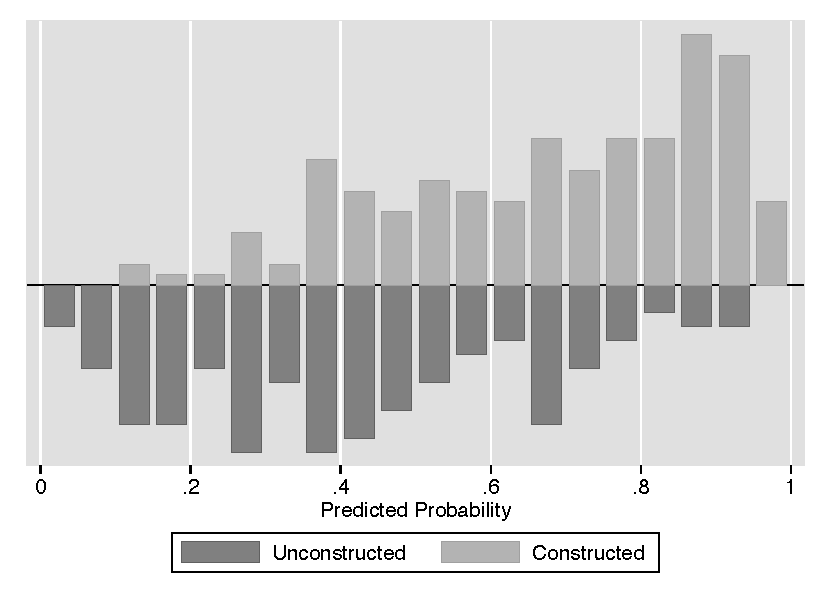
\includegraphics[scale=.8]{figures/psgraph.pdf}
{\footnotesize 
\begin{flushleft}
This Figure plots histograms of predicted probabilities of construction status according to the logistic regression with results in Table~\ref{table:pweight}.  Histograms are shown separately for constructed projects (top) and unconstructed projects (bottom).
\end{flushleft}}
\end{centering}
\end{figure}




\begin{table}[ht!]
\small
\centering
\caption{Results with Propensity Score Weighting}\label{table:mainpweight}
\vspace{-2mm}
\resizebox{1\linewidth}{!}{
\begin{threeparttable}
\begin{tabular}{lCCCCCC}
\toprule
                    &(1)&(2)&(3)&(4)&(5)&(6)\\[.5em] &Formal Houses                   &People in Formal Houses                    &Informal Houses                   &Informal Backyard Houses                    &Informal Non-Backyard Houses                    &People living in Informal Housing\\ \midrule                   \\
Post $\times$ Const.&        4.40\textsuperscript{a}&       18.71\textsuperscript{a}&        0.92                   &        3.44\textsuperscript{a}&       -2.52\textsuperscript{a}&       -3.24                   \\
                    &      (0.62)                   &      (2.12)                   &      (0.75)                   &      (0.80)                   &      (0.58)                   &      (1.68)                   \\
                    &      [0.00]                   &      [0.00]                   &      [0.22]                   &      [0.00]                   &      [0.00]                   &      [0.11]                   \\
Mean Pre            &        1.74                   &        9.50                   &        5.34                   &        0.52                   &        4.82                   &       13.60                   \\
Mean Post           &        5.68                   &       27.30                   &        8.62                   &        4.45                   &        4.17                   &       13.96                   \\
R$^2$               &       0.139                   &       0.168                   &       0.038                   &       0.123                   &       0.011                   &       0.014                   \\
N                   &      85,944                   &      79,629                   &      85,944                   &      85,944                   &      85,944                   &      79,629                   \\

\bottomrule
\\
                    &                               &                               &                               &                               &                               &                               \\
Post $\times$ Const. (0-.5 km)&        0.20\textsuperscript{b}&        1.57\textsuperscript{a}&        0.12                   &        0.17                   &       -0.06                   &       -0.33                   \\
                    &      (0.10)                   &      (0.52)                   &      (0.20)                   &      (0.14)                   &      (0.15)                   &      (0.54)                   \\
                    &      [0.04]                   &      [0.00]                   &      [0.56]                   &      [0.21]                   &      [0.71]                   &      [0.55]                   \\
Mean Pre            &        1.83                   &        9.53                   &        0.95                   &        0.53                   &        0.42                   &        2.61                   \\
Mean Post           &        2.09                   &       12.91                   &        1.74                   &        1.22                   &        0.52                   &        2.82                   \\
R$^2$               &       0.030                   &       0.027                   &       0.035                   &       0.035                   &       0.010                   &       0.014                   \\
N                   &     774,416                   &     620,169                   &     774,416                   &     774,416                   &     774,416                   &     620,169                   \\

\bottomrule
\end{tabular}
\begin{tablenotes}
\item \footnotesize 
This table shows the direct and spillover effects of constructed housing projects on population and housing outcomes where observations are weighted by their propensity scores calculated from predicted values in Table~\ref{table:pweight}. \regtextfirst  The Bonferonni correction is calculated separately for columns (1) to (6) and (7) to (12).
\end{tablenotes}
\end{threeparttable}
}
\end{table}



\begin{table}
\small
\centering
\caption{Census Results with 1996 as the Pre-Period and 2001 as the Post-Period}\label{table:mainplacebo}
\vspace{-2mm}
\resizebox{1\linewidth}{!}{
\begin{threeparttable}
\begin{tabular}{lCCCCCC}

% \textbf{Direct Effects} \\
\toprule
                    &(1)&(2)&(3)&(4)&(5)\\[.5em] &People in Formal Housing                   &People in Informal Housing                   &Electric Lighting                   &Flush Toilet                   &Piped Water Inside\\ \midrule                    \\
Post $\times$ Const.&        3.91\textsuperscript{a}&       -1.08                   &        0.10                   &        0.07                   &        0.01                   \\
                    &      (1.10)                   &      (1.56)                   &      (0.07)                   &      (0.07)                   &      (0.05)                   \\
                    &      [0.00]                   &      [1.00]                   &      [0.72]                   &      [1.00]                   &      [1.00]                   \\
Mean Pre            &        5.11                   &       12.58                   &        0.53                   &        0.56                   &        0.37                   \\
Mean Post           &        9.49                   &       13.59                   &        0.54                   &        0.57                   &        0.26                   \\
R$^2$               &       0.041                   &       0.076                   &       0.023                   &       0.016                   &       0.071                   \\
N                   &      75,251                   &      75,251                   &      75,251                   &      75,251                   &      75,251                   \\

\\
\textbf{Spillover Effects} \\\midrule
                    &                               &                               &                               &                               &                               \\
Post $\times$ Const. (0-.5 km)&        0.20                   &       -0.20                   &        0.01                   &       -0.00                   &        0.01                   \\
                    &      (0.39)                   &      (0.37)                   &      (0.01)                   &      (0.01)                   &      (0.01)                   \\
                    &      [0.61]                   &      [0.59]                   &      [0.26]                   &      [0.89]                   &      [0.57]                   \\
Mean Pre            &        8.16                   &        2.36                   &        0.67                   &        0.67                   &        0.55                   \\
Mean Post           &        9.52                   &        2.61                   &        0.71                   &        0.72                   &        0.43                   \\
R$^2$               &       0.030                   &       0.015                   &       0.015                   &       0.008                   &       0.039                   \\
N                   &     642,648                   &     642,648                   &     642,549                   &     642,549                   &     642,549                   \\

\bottomrule
\end{tabular}
\begin{tablenotes}
\item \footnotesize This table shows the direct and spillover effects of constructed housing projects on population and housing outcomes where the pre-period (Post=0) is 1996 and the post-period is 2001 (Post=1). \regtextfirst The Bonferonni correction is calculated separately for columns (1) to (6) and (7) to (12).
\end{tablenotes}
\end{threeparttable}
}
\end{table}

\begin{table}
\small
\centering
\caption{Results with the 134 projects that are at least 2 km away from other projects}\label{table:far_robust}
\vspace{-2mm}
\resizebox{1\linewidth}{!}{
\begin{threeparttable}
\begin{tabular}{lCCCCCC}
% \textbf{Direct Effects} \\
\toprule
                    &(1)&(2)&(3)&(4)&(5)&(6)\\[.5em] &Formal Houses                   &People in Formal Houses                    &Informal Houses                   &Informal Backyard Houses                    &Informal Non-Backyard Houses                    &People living in Informal Housing\\ \midrule                   \\
Post $\times$ Const.&        4.30\textsuperscript{a}&       19.41\textsuperscript{a}&        1.38                   &        3.94\textsuperscript{a}&       -2.56\textsuperscript{a}&       -3.44                   \\
                    &      (0.67)                   &      (2.31)                   &      (0.80)                   &      (0.97)                   &      (0.76)                   &      (2.09)                   \\
                    &      [0.00]                   &      [0.00]                   &      [0.17]                   &      [0.00]                   &      [0.00]                   &      [0.17]                   \\
Mean Pre            &        1.57                   &        8.96                   &        4.27                   &        0.55                   &        3.73                   &       10.85                   \\
Mean Post           &        5.19                   &       24.97                   &        6.65                   &        3.71                   &        2.94                   &       10.61                   \\
R$^2$               &       0.187                   &       0.234                   &       0.063                   &       0.146                   &       0.024                   &       0.034                   \\
N                   &      56,510                   &      51,596                   &      56,510                   &      56,510                   &      56,510                   &      51,596                   \\

\\
\textbf{Spillover Effects} \\\midrule
                    &                               &                               &                               &                               &                               &                               \\
Post $\times$ Const. (0-.5 km)&        0.19                   &        0.88\textsuperscript{c}&        0.46\textsuperscript{b}&        0.35\textsuperscript{b}&        0.11                   &        0.43                   \\
                    &      (0.12)                   &      (0.46)                   &      (0.20)                   &      (0.14)                   &      (0.17)                   &      (0.45)                   \\
                    &      [0.12]                   &      [0.06]                   &      [0.02]                   &      [0.01]                   &      [0.52]                   &      [0.34]                   \\
Mean Pre            &        1.81                   &        9.56                   &        1.17                   &        0.52                   &        0.65                   &        3.31                   \\
Mean Post           &        2.22                   &       13.66                   &        2.10                   &        1.37                   &        0.73                   &        3.56                   \\
R$^2$               &       0.061                   &       0.050                   &       0.077                   &       0.065                   &       0.032                   &       0.044                   \\
N                   &     815,268                   &     649,799                   &     815,268                   &     815,268                   &     815,268                   &     649,799                   \\

\bottomrule
\end{tabular}
\begin{tablenotes}
\item \footnotesize This table shows the direct and spillover effects of constructed housing projects on population and housing outcomes excluding overlap with the 134 projects that are within 2 km of another project. \regtextfirst  The Bonferonni correction is calculated separately for columns (1) to (6) and (7) to (12).
\end{tablenotes}
\end{threeparttable}
}
\end{table}


\begin{table}
\small
\centering
\caption{Results excluding overlap with 89 ``Proposed,'' ``Investigating,'' and ``Uncertain'' Unconstructed Projects}\label{table:dropplacebo_robust}
\vspace{-2mm}
\resizebox{1\linewidth}{!}{
\begin{threeparttable}
\begin{tabular}{lCCCCCC}

% \textbf{Direct Effects} \\
\toprule
                    &(1)&(2)&(3)&(4)&(5)&(6)\\[.5em] &Formal Houses                   &People in Formal Houses                    &Informal Houses                   &Informal Backyard Houses                    &Informal Non-Backyard Houses                    &People living in Informal Housing\\ \midrule                   \\
Post $\times$ Const.&        4.42\textsuperscript{a}&       20.37\textsuperscript{a}&        1.67\textsuperscript{c}&        4.35\textsuperscript{a}&       -2.68\textsuperscript{a}&       -2.98                   \\
                    &      (0.57)                   &      (1.94)                   &      (0.79)                   &      (0.80)                   &      (0.65)                   &      (1.86)                   \\
                    &      [0.00]                   &      [0.00]                   &      [0.07]                   &      [0.00]                   &      [0.00]                   &      [0.11]                   \\
Mean Pre            &        1.91                   &       10.57                   &        6.13                   &        0.60                   &        5.53                   &       15.80                   \\
Mean Post           &        6.46                   &       30.90                   &        9.63                   &        5.18                   &        4.46                   &       15.19                   \\
R$^2$               &       0.172                   &       0.210                   &       0.069                   &       0.157                   &       0.029                   &       0.037                   \\
N                   &      71,964                   &      66,542                   &      71,964                   &      71,964                   &      71,964                   &      66,542                   \\

\\
\textbf{Spillover Effects} \\\midrule
                    &                               &                               &                               &                               &                               &                               \\
Post $\times$ Const. (0-.5 km)&        0.29\textsuperscript{b}&        1.61\textsuperscript{a}&        0.41\textsuperscript{b}&        0.30\textsuperscript{b}&        0.10                   &        0.34                   \\
                    &      (0.13)                   &      (0.56)                   &      (0.20)                   &      (0.14)                   &      (0.16)                   &      (0.49)                   \\
                    &      [0.03]                   &      [0.00]                   &      [0.05]                   &      [0.03]                   &      [0.53]                   &      [0.49]                   \\
Mean Pre            &        1.79                   &        9.40                   &        0.94                   &        0.51                   &        0.43                   &        2.61                   \\
Mean Post           &        2.05                   &       12.78                   &        1.74                   &        1.19                   &        0.55                   &        2.91                   \\
R$^2$               &       0.049                   &       0.038                   &       0.042                   &       0.046                   &       0.010                   &       0.015                   \\
N                   &     799,814                   &     634,853                   &     799,814                   &     799,814                   &     799,814                   &     634,853                   \\

\bottomrule
\end{tabular}
\begin{tablenotes}
\item \footnotesize  This table shows the direct and spillover effects of constructed housing projects on population and housing outcomes where overlap with 71 unconstructed projects labeled ``proposed'' is excluded. \regtextfirst  The Bonferonni correction is calculated separately for columns (1) to (6) and (7) to (12).
\end{tablenotes}
\end{threeparttable}
}
\end{table}


\begin{table}
\small
\centering
\caption{Results with Time-Varying Geographic Controls}\label{table:timevar}
\vspace{-2mm}
\resizebox{1\linewidth}{!}{
\begin{threeparttable}
\begin{tabular}{lCCCCCC}

% \textbf{Direct Effects} \\
\toprule
                    &(1)&(2)&(3)&(4)&(5)&(6)\\[.5em] &Formal Houses                   &People in Formal Houses                    &Informal Houses                   &Informal Backyard Houses                    &Informal Non-Backyard Houses                    &People living in Informal Housing\\ \midrule                   \\
Post $\times$ Const.&        4.63\textsuperscript{a}&       20.88\textsuperscript{a}&        2.15\textsuperscript{a}&        5.12\textsuperscript{a}&       -2.97\textsuperscript{a}&       -4.11\textsuperscript{b}\\
                    &      (0.53)                   &      (1.84)                   &      (0.70)                   &      (0.84)                   &      (0.61)                   &      (1.71)                   \\
                    &      [0.00]                   &      [0.00]                   &      [0.00]                   &      [0.00]                   &      [0.00]                   &      [0.02]                   \\
Mean Pre            &        1.73                   &        9.49                   &        5.32                   &        0.52                   &        4.80                   &       13.59                   \\
Mean Post           &        5.65                   &       27.29                   &        8.57                   &        4.42                   &        4.15                   &       13.96                   \\
R$^2$               &       0.191                   &       0.245                   &       0.106                   &       0.192                   &       0.046                   &       0.067                   \\
N                   &      86,442                   &      79,688                   &      86,442                   &      86,442                   &      86,442                   &      79,688                   \\

\\
\textbf{Spillover Effects} \\\midrule
                    &                               &                               &                               &                               &                               &                               \\
Post $\times$ Const. (0-.5 km)&        0.22\textsuperscript{b}&        1.31\textsuperscript{a}&        0.44\textsuperscript{b}&        0.34\textsuperscript{a}&        0.09                   &        0.57                   \\
                    &      (0.10)                   &      (0.47)                   &      (0.17)                   &      (0.12)                   &      (0.15)                   &      (0.42)                   \\
                    &      [0.03]                   &      [0.01]                   &      [0.01]                   &      [0.01]                   &      [0.53]                   &      [0.18]                   \\
Mean Pre            &        1.81                   &        9.52                   &        0.94                   &        0.52                   &        0.41                   &        2.61                   \\
Mean Post           &        2.06                   &       12.87                   &        1.72                   &        1.20                   &        0.52                   &        2.83                   \\
R$^2$               &       0.085                   &       0.090                   &       0.051                   &       0.059                   &       0.011                   &       0.024                   \\
N                   &     785,336                   &     621,707                   &     785,336                   &     785,336                   &     785,336                   &     621,707                   \\

\bottomrule
\end{tabular}
\begin{tablenotes}
\item \footnotesize  This table shows the direct and spillover effects of constructed housing projects on population and housing outcomes where specifications control for distance to CBD, distance to main highways, elevation, and land slope as well as the interactions of these variables with $Post$. \regtextfirst  The Bonferonni correction is calculated separately for columns (1) to (6) and (7) to (12).
\end{tablenotes}
\end{threeparttable}
}
\end{table}



\begin{table}
\small
\centering
\caption{Census Results using Enumerator Areas instead of Plots}\label{table:census_ea_robust}
\vspace{-2mm}
\resizebox{1\linewidth}{!}{
\begin{threeparttable}
\begin{tabular}{lCCCCCC}

% \textbf{Direct Effects} \\
\toprule
                    &(1)&(2)&(3)&(4)&(5)\\[.5em] &People in Formal Housing                   &People in Informal Housing                   &Electric Lighting                   &Flush Toilet                   &Piped Water Inside\\ \midrule                    \\
Post $\times$ Const.&        0.88\textsuperscript{a}&       -1.21\textsuperscript{a}&        0.08\textsuperscript{b}&        0.13\textsuperscript{a}&        0.10\textsuperscript{a}\\
                    &      (0.23)                   &      (0.30)                   &      (0.04)                   &      (0.03)                   &      (0.03)                   \\
                    &      [0.00]                   &      [0.00]                   &      [0.04]                   &      [0.00]                   &      [0.00]                   \\
Mean Pre            &        2.87                   &        4.42                   &        0.62                   &        0.66                   &        0.23                   \\
Mean Post           &        5.60                   &        3.76                   &        0.74                   &        0.76                   &        0.43                   \\
R$^2$               &       0.128                   &       0.039                   &       0.025                   &       0.035                   &       0.075                   \\
N                   &       4,886                   &       4,886                   &       4,886                   &       4,886                   &       4,886                   \\

\\
\textbf{Spillover Effects} \\\midrule
                    &                               &                               &                               &                               &                               \\
Post $\times$ Const. (0-.5 km)&       -0.13                   &       -0.27                   &        0.00                   &       -0.03                   &        0.01                   \\
                    &      (0.23)                   &      (0.42)                   &      (0.02)                   &      (0.02)                   &      (0.02)                   \\
                    &      [0.58]                   &      [0.52]                   &      [0.97]                   &      [0.22]                   &      [0.66]                   \\
Mean Pre            &        6.40                   &        2.84                   &        0.86                   &        0.88                   &        0.50                   \\
Mean Post           &        5.86                   &        2.28                   &        0.89                   &        0.89                   &        0.69                   \\
R$^2$               &       0.028                   &       0.051                   &       0.030                   &       0.039                   &       0.115                   \\
N                   &       9,741                   &       9,741                   &       9,740                   &       9,740                   &       9,740                   \\

\bottomrule
\end{tabular}
\begin{tablenotes}
\item \footnotesize This table shows the direct and spillover effects of constructed housing projects on population and housing outcomes where the pre-period (Post=0) is 1996 and the post-period is 2001 (Post=1). \regtextfirst The Bonferonni correction is calculated separately for columns (1) to (6) and (7) to (12).
\end{tablenotes}
\end{threeparttable}
}
\end{table}

\begin{table}
\small
\centering
\caption{Results comparing houses in building data with households in census data}\label{table:census_building_robust}
\vspace{-2mm}
\resizebox{1\linewidth}{!}{
\begin{threeparttable}
\begin{tabular}{lEEEEEEE}

% \textbf{Direct Effects} \\
\toprule
                    &(1)&(2)&(3)&(4)&(5)&(6)&(7)\\[.5em]                 
                    &Formal Houses&Households in Formal Houses                   &Informal Houses                   &Households in Informal Houses                   &Backyard Informal Houses                   &Households in Backyard Shacks                   &Households in Backyard Houses                   \\[.5em]
    Dataset                                    &Building&Census&Building&Census&Building&Census&Census\\[.5em]   \midrule
Post $\times$ Const.&        4.43\textsuperscript{a}&        6.29\textsuperscript{a}&        1.65\textsuperscript{b}&       -0.29                   &        4.44\textsuperscript{a}&        1.15\textsuperscript{b}&        0.82\textsuperscript{b}\\
                    &      (0.54)                   &      (0.72)                   &      (0.69)                   &      (0.82)                   &      (0.77)                   &      (0.39)                   &      (0.33)                   \\
                    &      [0.00]                   &      [0.00]                   &      [0.04]                   &      [0.72]                   &      [0.00]                   &      [0.01]                   &      [0.04]                   \\
Mean Pre            &        1.73                   &        2.63                   &        5.32                   &        4.40                   &        0.52                   &        0.70                   &        0.16                   \\
Mean Post           &        5.65                   &        8.46                   &        8.57                   &        5.71                   &        4.42                   &        2.16                   &        0.78                   \\
R$^2$               &       0.178                   &       0.183                   &       0.084                   &       0.039                   &       0.166                   &       0.051                   &       0.045                   \\
N                   &      86,442                   &      79,462                   &      86,442                   &      79,462                   &      86,442                   &      79,462                   &      79,462                   \\

\\
\textbf{Spillover Effects} \\\midrule
                    &                               &                               &                               &                               &                               &                               &                               \\
Post $\times$ Const. (0-.5 km)&        0.22\textsuperscript{b}&        0.48\textsuperscript{a}&        0.43\textsuperscript{b}&        0.28                   &        0.34\textsuperscript{a}&        0.13                   &        0.16\textsuperscript{a}\\
                    &      (0.10)                   &      (0.16)                   &      (0.17)                   &      (0.18)                   &      (0.12)                   &      (0.10)                   &      (0.05)                   \\
                    &      [0.03]                   &      [0.00]                   &      [0.01]                   &      [0.12]                   &      [0.01]                   &      [0.22]                   &      [0.00]                   \\
Mean Pre            &        1.81                   &        2.58                   &        0.94                   &        1.00                   &        0.52                   &        0.29                   &        0.31                   \\
Mean Post           &        2.06                   &        4.08                   &        1.72                   &        1.25                   &        1.20                   &        0.42                   &        0.37                   \\
R$^2$               &       0.049                   &       0.031                   &       0.041                   &       0.013                   &       0.046                   &       0.008                   &       0.015                   \\
N                   &     785,336                   &     619,681                   &     785,336                   &     619,681                   &     785,336                   &     619,681                   &     619,681                   \\

\bottomrule
\end{tabular}
\begin{tablenotes}
\item \footnotesize This table shows the direct and spillover effects of constructed housing projects on houses in the building data and households measured in the census data.  \regtextfirst The Bonferonni correction is calculated separately for columns (1) to (6) and (7) to (12).
\end{tablenotes}
\end{threeparttable}
}
\end{table}

\begin{table}
\small
\centering
\caption{Spillover Effects by 0.1 km Rings from 0 to 0.5 km from Plots}\label{table:dist_robust}
\vspace{-2mm}
\resizebox{1\linewidth}{!}{
\begin{threeparttable}
\begin{tabular}{lCCCCC}
\toprule
                    &(1)&(2)&(3)&(4)&(5)\\[.5em] &Formal Houses                    &People in Formal Houses                   &Informal Backyard Houses                   &Informal Non-Backyard Houses                   &People in Informal Houses \\ \midrule                    \\
Post $\times$ Const. $\times$ Ring (km) \\\hspace{.5em}0-.1   &        0.08                   &        0.44                   &       -0.01                   &        0.01                   &       -0.26                   \\
                    &      (0.07)                   &      (0.52)                   &      (0.12)                   &      (0.16)                   &      (0.52)                   \\
\hspace{.5em}.1-.2  &       -0.08                   &        0.09                   &        0.05                   &       -0.12                   &        0.69                   \\
                    &      (0.09)                   &      (0.62)                   &      (0.14)                   &      (0.19)                   &      (0.61)                   \\
\hspace{.5em}.2-.3  &        0.08                   &        0.86                   &       -0.00                   &        0.10                   &       -0.59                   \\
                    &      (0.16)                   &      (0.79)                   &      (0.16)                   &      (0.21)                   &      (0.78)                   \\
\hspace{.5em}.3-.4  &        0.04                   &       -0.26                   &        0.05                   &        0.09                   &        0.98                   \\
                    &      (0.15)                   &      (0.84)                   &      (0.21)                   &      (0.21)                   &      (0.86)                   \\
\hspace{.5em}.4-.5  &        0.22\textsuperscript{c}&        1.01                   &        0.41\textsuperscript{b}&        0.02                   &       -0.11                   \\
                    &      (0.12)                   &      (0.88)                   &      (0.20)                   &      (0.18)                   &      (0.71)                   \\
Mean Pre            &        1.81                   &        9.52                   &        0.52                   &        0.41                   &        2.61                   \\
Mean Post           &        2.06                   &       12.87                   &        1.20                   &        0.52                   &        2.83                   \\
R$^2$               &       0.050                   &       0.040                   &       0.047                   &       0.009                   &       0.016                   \\
N                   &     785,336                   &     621,707                   &     785,336                   &     785,336                   &     621,707                   \\

\bottomrule
\end{tabular}
\begin{tablenotes}
\item \footnotesize  This table shows the spillover effects for 0.1 km rings from 0 to 0.5 km from plots.  The full set of 0.5 km rings from 0.5 to 4 km from plots are also included as controls although the coefficients are not included here.  \regtextfirst
\end{tablenotes}
\end{threeparttable}
}
\end{table}



\begin{table}[ht!]
\small
\centering
\caption{Correlations between Houses (Building Data) and Households (Census Data)  }\label{table:densitycorr}
\vspace{-2mm}
% \resizebox{1\linewidth}{!}{
\begin{threeparttable}
\begin{tabular}{lCC}
\toprule
 &Pre & Post \\
Average &  & \\
\midrule
Building Data  \\
\hspace{1cm} Formal House Density& 1.80 & 10.61 \\
\hspace{1cm} Informal House Density & 11.18 & 16.30 \\
Census Data  \\
\hspace{1cm} Households in Formal Housing Density& 2.37 & 18.68 \\
\hspace{1cm} Households in Informal Housing Density & 1.08 & 1.26 \\
\\
Correlation of Building Data and Census Data \\
\midrule
\hspace{1cm} Formal House/Household Density & . & . \\
\hspace{1cm} Informal House/Household Density & . & . \\
\bottomrule
\end{tabular}
\begin{tablenotes}
\item \footnotesize 
 This table shows average formal/informal house densities from the building data and densities of households living in formal/informal houses in the census data.  Densities are calculated at the of census enumerator areas. This table also shows correlations between these measures.
\end{tablenotes}
\end{threeparttable}
% }
\end{table}


\begin{table}[ht!]
\small
\centering
\caption{Correlations between Businesses (Building Data) and Economic Indicators (Census Data)  }\label{table:empcorr}
\vspace{-2mm}
% \resizebox{1\linewidth}{!}{
\begin{threeparttable}
\begin{tabular}{lCC}
\toprule
 &Pre & Post \\
Mean &  & \\
\midrule
Building Data  \\
\hspace{1cm} Business Density& 0.149 & 0.191 \\
\hspace{1cm} Informal Business Density & 0.012 & 0.035 \\
Census Data  \\
\hspace{1cm} Employment & 0.699 & 0.815 \\
\hspace{1cm} Log Income & 7.280 & 8.311 \\
\\
Correlation of Building Data and Census Data \\
\midrule
\hspace{1cm} Business Density and Employment & 0.061 & 0.035 \\
\hspace{1cm} Informal Building Density and Employment & -0.054 & -0.055 \\
\hspace{1cm} Business Density and Log Income & 0.027 & 0.003 \\
\hspace{1cm} Informal Building Density and Log Income & -0.042 & -0.095 \\
\bottomrule
\end{tabular}
\begin{tablenotes}
\item \footnotesize 
 This table shows average formal/informal businesses densities from the building data and average employment and log-income in the census data.  Densities are calculated at the of census enumerator areas. This table also shows correlations between these measures.
\end{tablenotes}
\end{threeparttable}
% }
\end{table}



\begin{table}[ht!]
\small
\centering
\caption{Correlations between Utilities (Building Data) and Access to Services (Census Data)   }\label{table:utilcorr}
\vspace{-2mm}
% \resizebox{1\linewidth}{!}{
\begin{threeparttable}
\begin{tabular}{lCC}
\toprule
 &Pre & Post \\
Mean &  & \\
\midrule
Building Data  \\
\hspace{1cm} Water Utility Buildings& 0.024 & 0.040 \\
\hspace{1cm} Electricity Utility Buildings& 0.004 & 0.006 \\
Census Data  \\
\hspace{1cm} Piped Water Inside & 0.42 & 0.61 \\
\hspace{1cm} Electric Lighting & 0.80 & 0.85 \\
\\
Correlation of Building Data and Census Data \\
\midrule
\hspace{1cm} Water Utility Buildings and Piped Water Inside & -0.031 & -0.035 \\
\hspace{1cm} Electricity Utility Buildings and Electric Lighting & 0.043 & 0.018 \\
\bottomrule
\end{tabular}
\begin{tablenotes}
\item \footnotesize 
 This table shows average utility building densities from the building data and basic service access in the census data.  Densities are calculated at the of census enumerator areas. This table also shows correlations between these measures.
\end{tablenotes}
\end{threeparttable}
% }
\end{table}









\begin{table}
\small
\centering
\caption{Direct Effects on Informal Housing and Demographics for All Inhabitants}\label{table:census_all_proj}
\vspace{-2mm}
\resizebox{1\linewidth}{!}{
\begin{threeparttable}
\begin{tabular}{lCCCCC}
\toprule
                    &(1)&(2)&(3)&(4)&(5)\\[.5em] &Total Rooms                   &   Own House                   &Electric Lighting                   &Flush Toilet                   &Piped Water Inside\\ \midrule                    \\
Post $\times$ Const.&        0.24                   &        0.03                   &        0.08\textsuperscript{c}&        0.16\textsuperscript{a}&        0.19\textsuperscript{a}\\
                    &      (0.20)                   &      (0.04)                   &      (0.04)                   &      (0.04)                   &      (0.04)                   \\
                    &      [0.46]                   &      [0.46]                   &      [0.10]                   &      [0.00]                   &      [0.00]                   \\
Mean Pre            &        2.90                   &        0.30                   &        0.54                   &        0.57                   &        0.26                   \\
Mean Post           &        3.34                   &        0.33                   &        0.68                   &        0.72                   &        0.46                   \\
R$^2$               &       0.052                   &       0.026                   &       0.058                   &       0.105                   &       0.126                   \\
N                   &      79,452                   &      79,675                   &      79,688                   &      79,688                   &      79,688                   \\

\\
\\\midrule
                    &(6)&(7)&(8)&(9)&(10)\\[.5em] &Age                   &     African                   &Household Size                   &  Employment                   &Log Income \\ \midrule                    \\
Post $\times$ Const.&       -0.60                   &       -0.01                   &        0.21                   &        0.02                   &        0.02                   \\
                    &      (0.61)                   &      (0.03)                   &      (0.10)                   &      (0.02)                   &      (0.12)                   \\
                    &      [1.00]                   &      [1.00]                   &      [0.20]                   &      [1.00]                   &      [1.00]                   \\
Mean Pre            &       39.98                   &        0.88                   &        3.13                   &        0.69                   &        7.07                   \\
Mean Post           &       40.93                   &        0.92                   &        2.89                   &        0.78                   &        7.88                   \\
R$^2$               &       0.022                   &       0.083                   &       0.098                   &       0.089                   &       0.356                   \\
N                   &      79,676                   &      79,688                   &      79,677                   &      79,338                   &      79,658                   \\

\bottomrule
\end{tabular}
\begin{tablenotes}
\item \footnotesize  This table shows the difference-in-differences coefficients for census measures for plots that overlap with projects.  Age, African, and employment are measured for the household head.  Employment is calculated for heads of household between ages 18 to 65.  Log income is measured at the household level.   \regtextfirst The Bonferroni correction is computed separately for columns 1-5 and columns 6-10.
\end{tablenotes}
\end{threeparttable}
}
\end{table}

\clearpage

\begin{table}
\small
\centering
\caption{Spillover Effects on Informal Housing and Demographics for Inhabitants}\label{table:census_informal_spill}
\vspace{-2mm}
\resizebox{1\linewidth}{!}{
\begin{threeparttable}
\begin{tabular}{lCCCCC}
\toprule
                    &(1)&(2)&(3)&(4)&(5)\\[.5em] &Total Rooms                   &   Own House                   &Electric Lighting                   &Flush Toilet                   &Piped Water Inside\\ \midrule                    \\
Post $\times$ Const. (0-.5 km)&        0.02                   &       -0.01                   &        0.00                   &        0.02\textsuperscript{c}&        0.01                   \\
                    &      (0.02)                   &      (0.01)                   &      (0.01)                   &      (0.01)                   &      (0.01)                   \\
                    &      [0.30]                   &      [0.47]                   &      [0.73]                   &      [0.09]                   &      [0.18]                   \\
Mean Pre            &        2.22                   &        0.18                   &        0.56                   &        0.60                   &        0.27                   \\
Mean Post           &        2.47                   &        0.19                   &        0.67                   &        0.62                   &        0.40                   \\
R$^2$               &       0.023                   &       0.005                   &       0.025                   &       0.008                   &       0.052                   \\
N                   &     565,966                   &     566,013                   &     566,013                   &     566,013                   &     566,013                   \\

\\
\\\midrule
                    &(6)&(7)&(8)&(9)&(10)\\[.5em] &Age                   &     African                   &Household Size                   &  Employment                   &Log Income \\ \midrule                    \\
Post $\times$ Const. (0-.5 km)&        0.21                   &        0.00                   &        0.00                   &        0.01                   &       -0.01                   \\
                    &      (0.15)                   &      (0.00)                   &      (0.02)                   &      (0.01)                   &      (0.02)                   \\
                    &      [0.15]                   &      [0.24]                   &      [0.87]                   &      [0.38]                   &      [0.62]                   \\
Mean Pre            &       39.49                   &        0.86                   &        2.58                   &        0.80                   &        6.89                   \\
Mean Post           &       39.90                   &        0.85                   &        2.35                   &        0.87                   &        7.99                   \\
R$^2$               &       0.018                   &       0.032                   &       0.024                   &       0.063                   &       0.314                   \\
N                   &     565,179                   &     566,013                   &     566,013                   &     555,371                   &     556,765                   \\

\bottomrule
\end{tabular}
\begin{tablenotes}
\item \footnotesize  This table shows the difference-in-differences coefficients for census measures for people living in informal housing.  The estimates are for plots that are outside of projects, but have at least one .5 km neighborhood ring that overlaps with a project.  Age, African, and employment are measured for the household head.  Employment is calculated for heads of household between ages 18 to 65.  Log income is measured at the household level.   \regtextfirst The Bonferroni correction is computed separately for columns 1-5 and columns 6-10.
\end{tablenotes}
\end{threeparttable}
}
\end{table}


\begin{table}
\small
\centering
\caption{Spillover Effects on Formal Housing and Demographics for Inhabitants}\label{table:census_formal_spill}
\vspace{-2mm}
\resizebox{1\linewidth}{!}{
\begin{threeparttable}
\begin{tabular}{lCCCCC}
\toprule
                    &(1)&(2)&(3)&(4)&(5)\\[.5em] &Total Rooms                   &   Own House                   &Electric Lighting                   &Flush Toilet                   &Piped Water Inside\\ \midrule                    \\
Post $\times$ Const. (0-.5 km)&        0.04                   &        0.01                   &        0.01                   &        0.01                   &        0.01                   \\
                    &      (0.03)                   &      (0.01)                   &      (0.01)                   &      (0.01)                   &      (0.01)                   \\
                    &      [0.12]                   &      [0.19]                   &      [0.25]                   &      [0.13]                   &      [0.34]                   \\
Mean Pre            &        3.99                   &        0.44                   &        0.78                   &        0.77                   &        0.49                   \\
Mean Post           &        4.37                   &        0.37                   &        0.83                   &        0.81                   &        0.66                   \\
R$^2$               &       0.027                   &       0.017                   &       0.023                   &       0.014                   &       0.087                   \\
N                   &     615,273                   &     615,713                   &     615,614                   &     615,614                   &     615,614                   \\

\\
\\\midrule
                    &(6)&(7)&(8)&(9)&(10)\\[.5em] &Age                   &     African                   &Household Size                   &  Employment                   &Log Income \\ \midrule                    \\
Post $\times$ Const. (0-.5 km)&        0.11                   &       -0.01                   &        0.03\textsuperscript{c}&        0.00                   &        0.00                   \\
                    &      (0.11)                   &      (0.00)                   &      (0.02)                   &      (0.00)                   &      (0.01)                   \\
                    &      [0.29]                   &      [0.17]                   &      [0.10]                   &      [0.22]                   &      [0.86]                   \\
Mean Pre            &       42.83                   &        0.63                   &        3.28                   &        0.84                   &        7.50                   \\
Mean Post           &       43.94                   &        0.67                   &        2.90                   &        0.88                   &        8.62                   \\
R$^2$               &       0.021                   &       0.094                   &       0.081                   &       0.100                   &       0.362                   \\
N                   &     614,415                   &     615,713                   &     615,511                   &     612,975                   &     614,144                   \\

\bottomrule
\end{tabular}
\begin{tablenotes}
\item \footnotesize  This table shows the difference-in-differences coefficients for census measures for people living in formal housing.  The estimates are for plots that are outside of projects, but have at least one .5 km neighborhood ring that overlaps with a project.  Age, African, and employment are measured for the household head.  Employment is calculated for heads of household between ages 18 to 65.  Log income is measured at the household level.   \regtextfirst The Bonferroni correction is computed separately for columns 1-5 and columns 6-10.
\end{tablenotes}
\end{threeparttable}
}
\end{table}






% \clearpage




% \begin{table}
% \small
% \centering
% \caption{Distribution of normalized exposure measures}\label{table:spatialsummaryexposure}
% \vspace{-2mm}
% % \resizebox{1\linewidth}{!}{
% \begin{threeparttable}
% \begin{tabular}{lrrrrrrrr}
% \toprule
%  & \multicolumn{4}{c}{Any Project Exposure} & \multicolumn{4}{c}{Constructed Exposure}  \\\cmidrule(lr){2-5}\cmidrule(lr){6-9}
% \\[-.7em]
% & Mean & SD & Max & N & Mean & SD & Max & N \\
% \midrule
%  Plot  & 1.24   & 0.46   & 1.49   & 39,472   & 1.23   & 0.47   & 1.49   & 48,152   \\[.15em] 

% \\[-.5em]
% Plot rings (km) \\
%  \hspace{1em}0-.5  & 1.44   & 1.34   & 8.81   & 109,786   & 1.41   & 1.31   & 8.42   & 60,670   \\[.15em] 
 \hspace{1em}.5-1  & 1.86   & 1.81   & 11.97   & 218,976   & 1.75   & 1.71   & 11.95   & 126,822   \\[.15em] 
 \hspace{1em}1-1.5  & 2.32   & 2.29   & 15.27   & 319,392   & 2.11   & 2.09   & 14.50   & 193,912   \\[.15em] 
 \hspace{1em}1.5-2  & 2.79   & 2.72   & 17.86   & 407,648   & 2.44   & 2.38   & 15.21   & 259,222   \\[.15em] 
 \hspace{1em}2-2.5  & 3.19   & 3.12   & 19.90   & 490,450   & 2.71   & 2.60   & 16.77   & 323,570   \\[.15em] 
 \hspace{1em}2.5-3  & 3.56   & 3.48   & 23.02   & 568,330   & 2.94   & 2.79   & 21.88   & 385,004   \\[.15em] 
 \hspace{1em}3-3.5  & 3.92   & 3.80   & 25.71   & 639,478   & 3.12   & 2.91   & 21.97   & 445,780   \\[.15em] 
 \hspace{1em}3.5-4  & 4.22   & 4.09   & 30.73   & 707,588   & 3.25   & 3.00   & 21.99   & 507,510   \\[.15em] 
	
% \bottomrule
% \end{tabular}
% \begin{tablenotes}
% \item \footnotesize  test here
% \end{tablenotes}
% \end{threeparttable}
% % }
% \end{table}












%%%%%%%%%%%% OLD FIGURESSS! !!!! %%%%%%%%%%%%%%%
%%%%%%%%%%%% OLD FIGURESSS! !!!! %%%%%%%%%%%%%%%
%%%%%%%%%%%% OLD FIGURESSS! !!!! %%%%%%%%%%%%%%%
%%%%%%%%%%%% OLD FIGURESSS! !!!! %%%%%%%%%%%%%%%


% \begin{figure}[ht!]
% \caption{Transaction Price Histogram}\label{figure:transactionhist}
% \centering
% 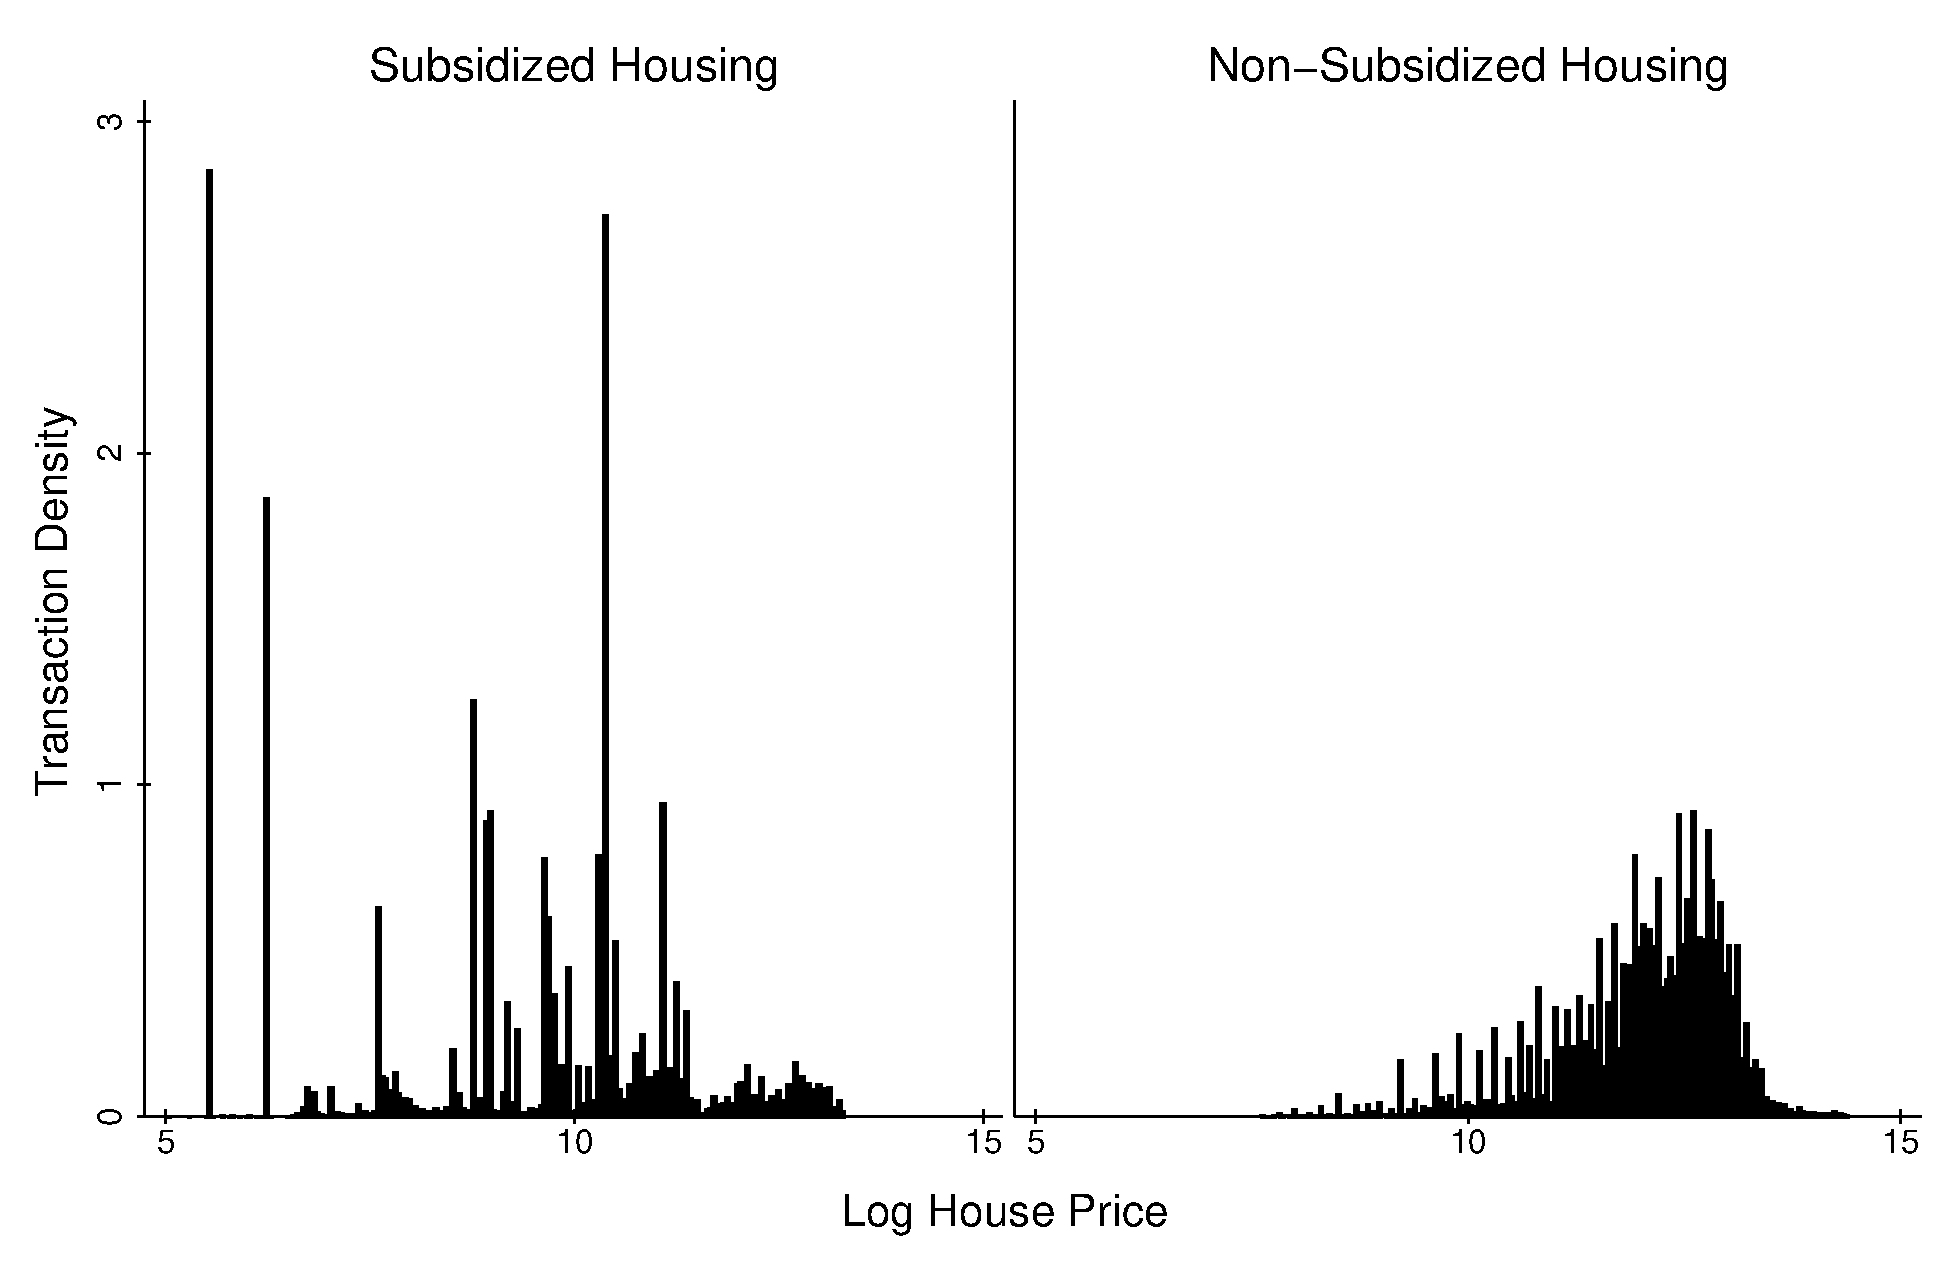
\includegraphics[scale=.4,trim={0cm 0cm -1cm 0cm}]{figures/summary_pricedist.pdf}
% \\
% \footnotesize{Note: Transactions are censored at R100,000.}
% \end{figure}

% \begin{figure}[h!]
% \centering
% \caption{Housing Transactions relative to Each Project's Modal Transaction Month}
% \label{appendix:histfreq}
% 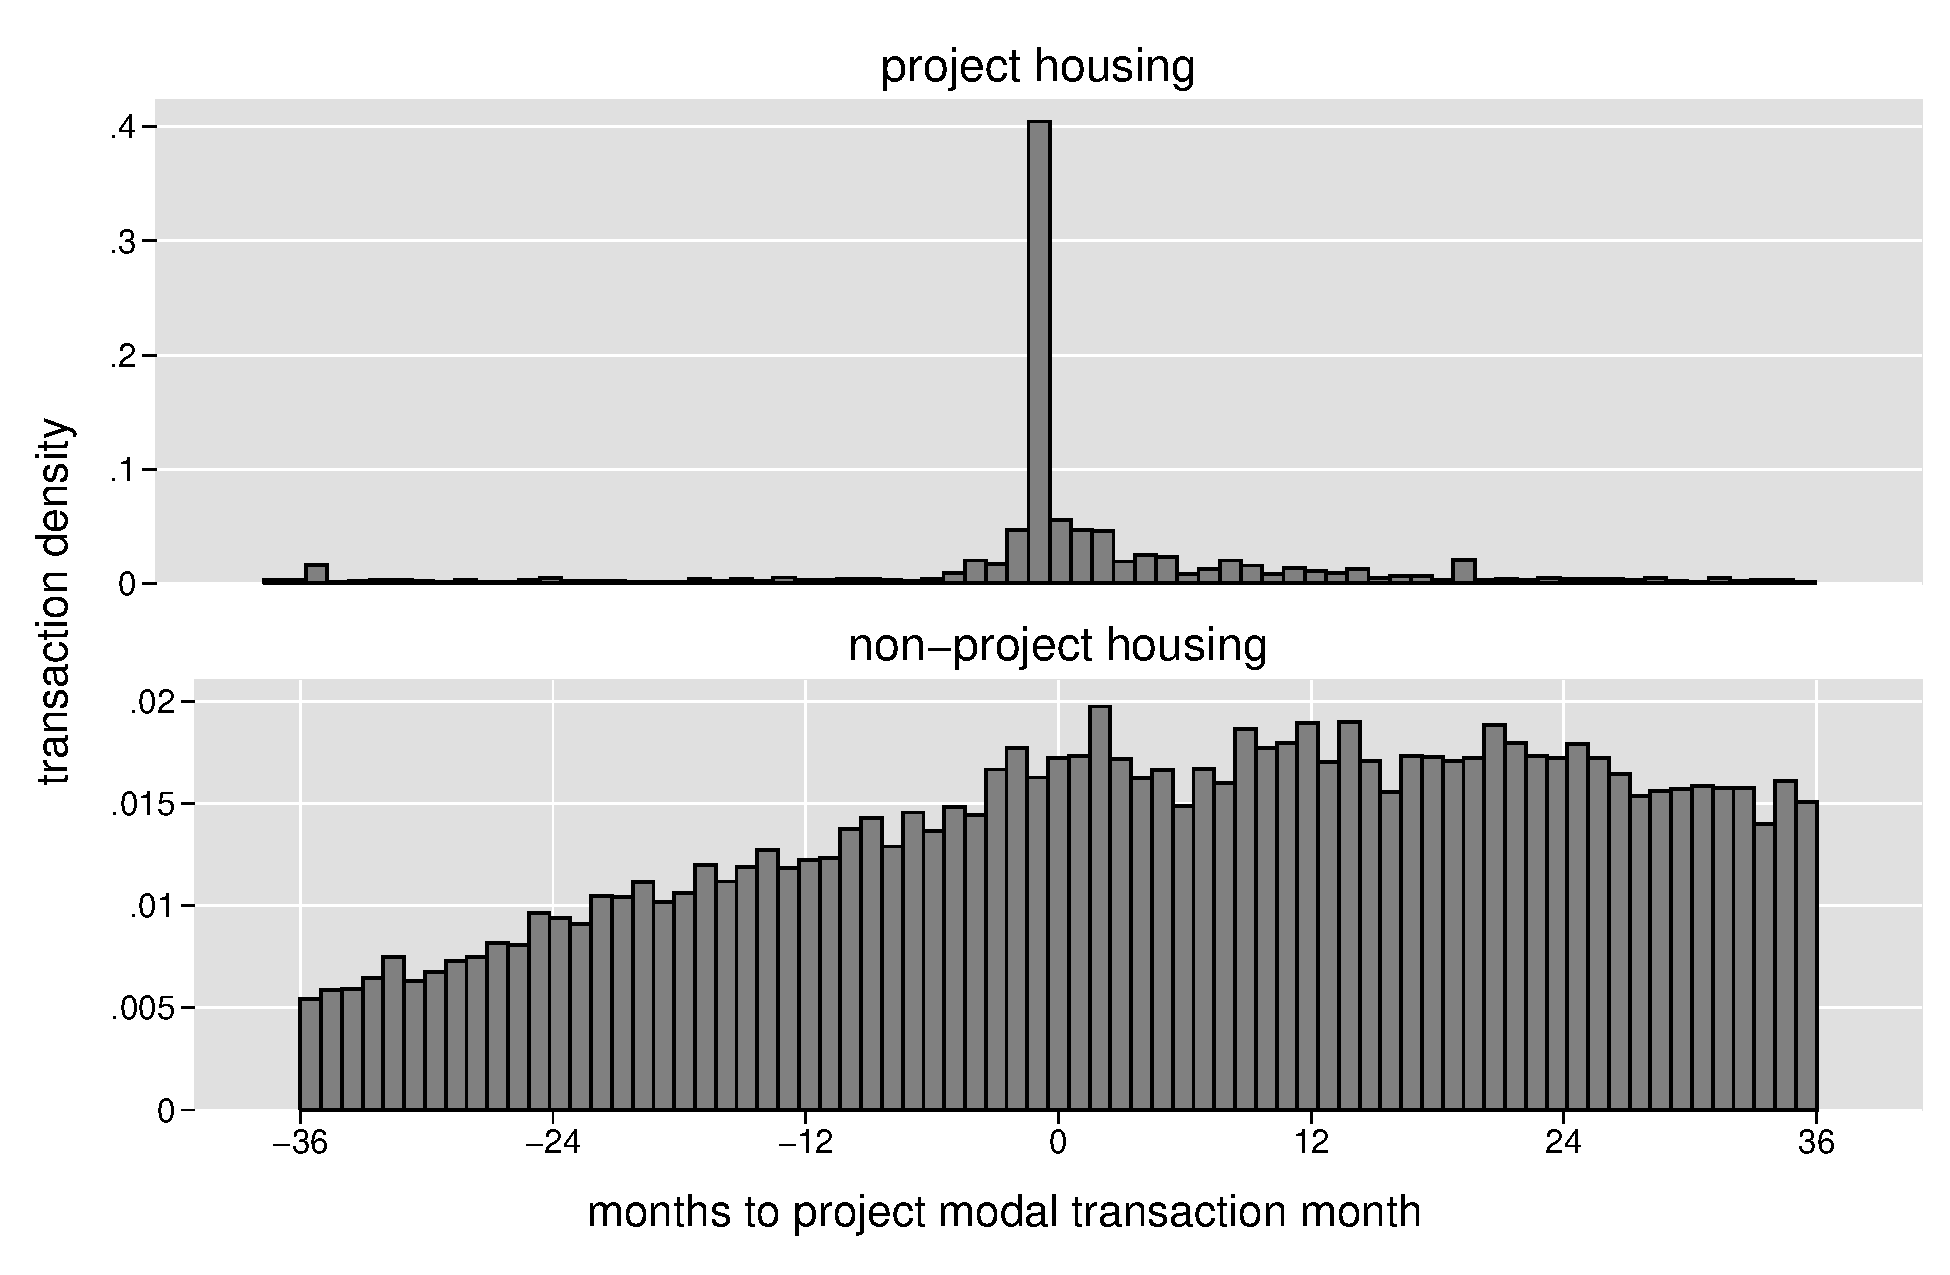
\includegraphics[scale=.4 , trim={.2cm 0.2cm .2cm 0.2cm},clip]{figures/summary_densitytime.pdf}
% \end{figure}





% \subsection{String Matching for Project Names and Delivery Dates }
% \label{appendix:stringmatch}


% We then use a fuzzy-string matching algorithm with bigrams to link project names from the budget reports to the administrative maps.  We keep all matches with over 60\% similarity, with 37 projects matching exactly.  Appendix~\ref{table:stringmatch} compares unmatched and matched projects finding that matched projects have much higher numbers of project houses, lower nearby housing prices, and are further from the central business district compared to unmatched projects.  One reason may be that the budget reports only include larger, more expansive projects, which are likely to take place further from city centers. 


% \vspace{0mm}
% \begin{table}[h!]
% \centering
% \caption{Assessing Name Matching between Budget Reports and Administrative Project Records}\label{table:stringmatch}
% \vspace{0mm}
% \begin{tabular}{l*{1}{cccc}}
% \toprule
%   & \multicolumn{2}{c}{\textbf{Matched}}& \multicolumn{2}{c}{\textbf{Unmatched}}    \\
%   &Const. & Unconst. &Const. & Unconst.  \\
% \midrule
%  Number of Projects  & 126  & 73  & 46  & 72  \\ 
 Area (km2)  & 1.22  & 1.02  & 1.05  & 1.30  \\ 
 Delivered Houses  & 416  & 15  & 259  & 7  \\ 
 House Price in 1 km (R$^\dagger$)  & 183,930  & 206,496  & 199,923  & 232,166  \\ 
 Distance to CBD$^\ddagger$ (km)  & 34.3  & 31.3  & 27.5  & 24.0  \\ 

% \bottomrule
% \multicolumn{5}{l}{\scriptsize Const. refers to constructed projects and unconst. refers to unconstructed projects.}\\[-.5em]
% \multicolumn{5}{l}{\scriptsize $^*$Calculated from {\it expected} completion dates using Gauteng National Treasury budget reports.}\\[-.5em]
% \multicolumn{5}{l}{\scriptsize $^\dagger$ The USD averaged to about 7.70 Rands during the 2001-2011 period.}\\[-.5em]
% \multicolumn{5}{l}{\scriptsize $^\ddagger$Measured as the average minimum distance with respect to Johannesburg and Pretoria CBDs. } \\[-.5em]
% \end{tabular}
% \end{table} 











% \subsection{Project counts}
% \label{appendix:projectcounts}
% \vspace{-5mm}
% \begin{figure}[ht!]
% \centering
% 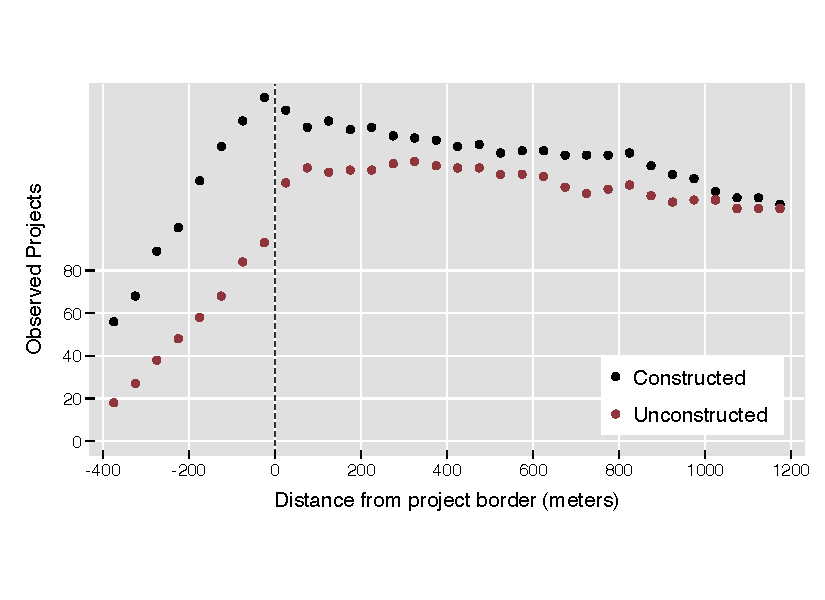
\includegraphics[scale=1.2,trim={.1cm 1.2cm .1cm 1.2cm},clip]{figures/projectcounts_4.pdf}
% \end{figure}




\end{document}


